% Created 2017-11-21 Tue 12:56
% Intended LaTeX compiler: pdflatex
\documentclass[titlepage]{article}
\usepackage[utf8]{inputenc}
\usepackage[T1]{fontenc}
\usepackage{graphicx}
\usepackage{grffile}
\usepackage{longtable}
\usepackage{wrapfig}
\usepackage{rotating}
\usepackage[normalem]{ulem}
\usepackage{amsmath}
\usepackage{textcomp}
\usepackage{amssymb}
\usepackage{capt-of}
\usepackage{hyperref}
\hypersetup{hidelinks=true}
\setlength{\parindent}{2em}
\usepackage[margin=1in]{geometry}
\usepackage[toc,page]{appendix}
\author{Hu Xiaoxiang \\
U1521319A \\
EEE \\
}
\date{11 Nov, 2017 \\
}
\title{
\includegraphics[width=\textwidth]{logo_ntu_new.png} \\
[5\baselineskip] EE4476 \\
REPORT \\
[5\baselineskip]}
\hypersetup{
 pdfauthor={Hu Xiaoxiang \\
U1521319A \\
EEE \\
},
 pdftitle={
\includegraphics[width=\textwidth]{logo_ntu_new.png} \\
[5\baselineskip] EE4476 \\
REPORT \\
[5\baselineskip]},
 pdfkeywords={},
 pdfsubject={},
 pdfcreator={Emacs 25.1.1 (Org mode 9.1.2)}, 
 pdflang={English}}
\begin{document}

\maketitle
\tableofcontents

\pagenumbering{roman}
\newpage
\pagenumbering{arabic}

\section{Introduction}
\label{sec:org1e6f45b}
With the proliferation of digital text sources in recent decades, such as the
Internet and the mobile phone, there is a increasing need for document image
processing and optical character recognition (OCR). However, many of the
original document images are distorted due to noise, under exposure, or motion
blur. Because of the different types of degradation in different images, each
category of them has to be treated separately. This report includes the
procedures which I used to process the given sample images, as well as the
source code of the process algorithms.

\section{Procedures And Algorithm}
\label{sec:org2b46001}
In this project, most of the algorithms are implemented in Python, while some
of the processes still require to use Matlab function, which is implemented
through Matlab Python API. 

To binarize a color image, the first step is to change the color map from
'RGB' to 'Gray Level'. In Python, 'pillow' is one of the basic image
processing libraries for image reading and color map converting. According to
its documentation, when translating a color image to black and white, the
library uses the ITU-R 601-2 luma transform:

$$ L = 0.299 * R + 0.587 * G + 0.114 * B $$

The histogram of image 1, 2, 3 is shown as below. The peak in the histogram is
the background. It shows that these three images have relatively high contrast
between its text and background. After several experiment of different
methods, it finally turns out that the n-bit slicing method performs best.
Note that 'im\(_{\text{np}}\)' in the source code is a 'numpy' array, which is used to
store images' gray value.

\begin{center}
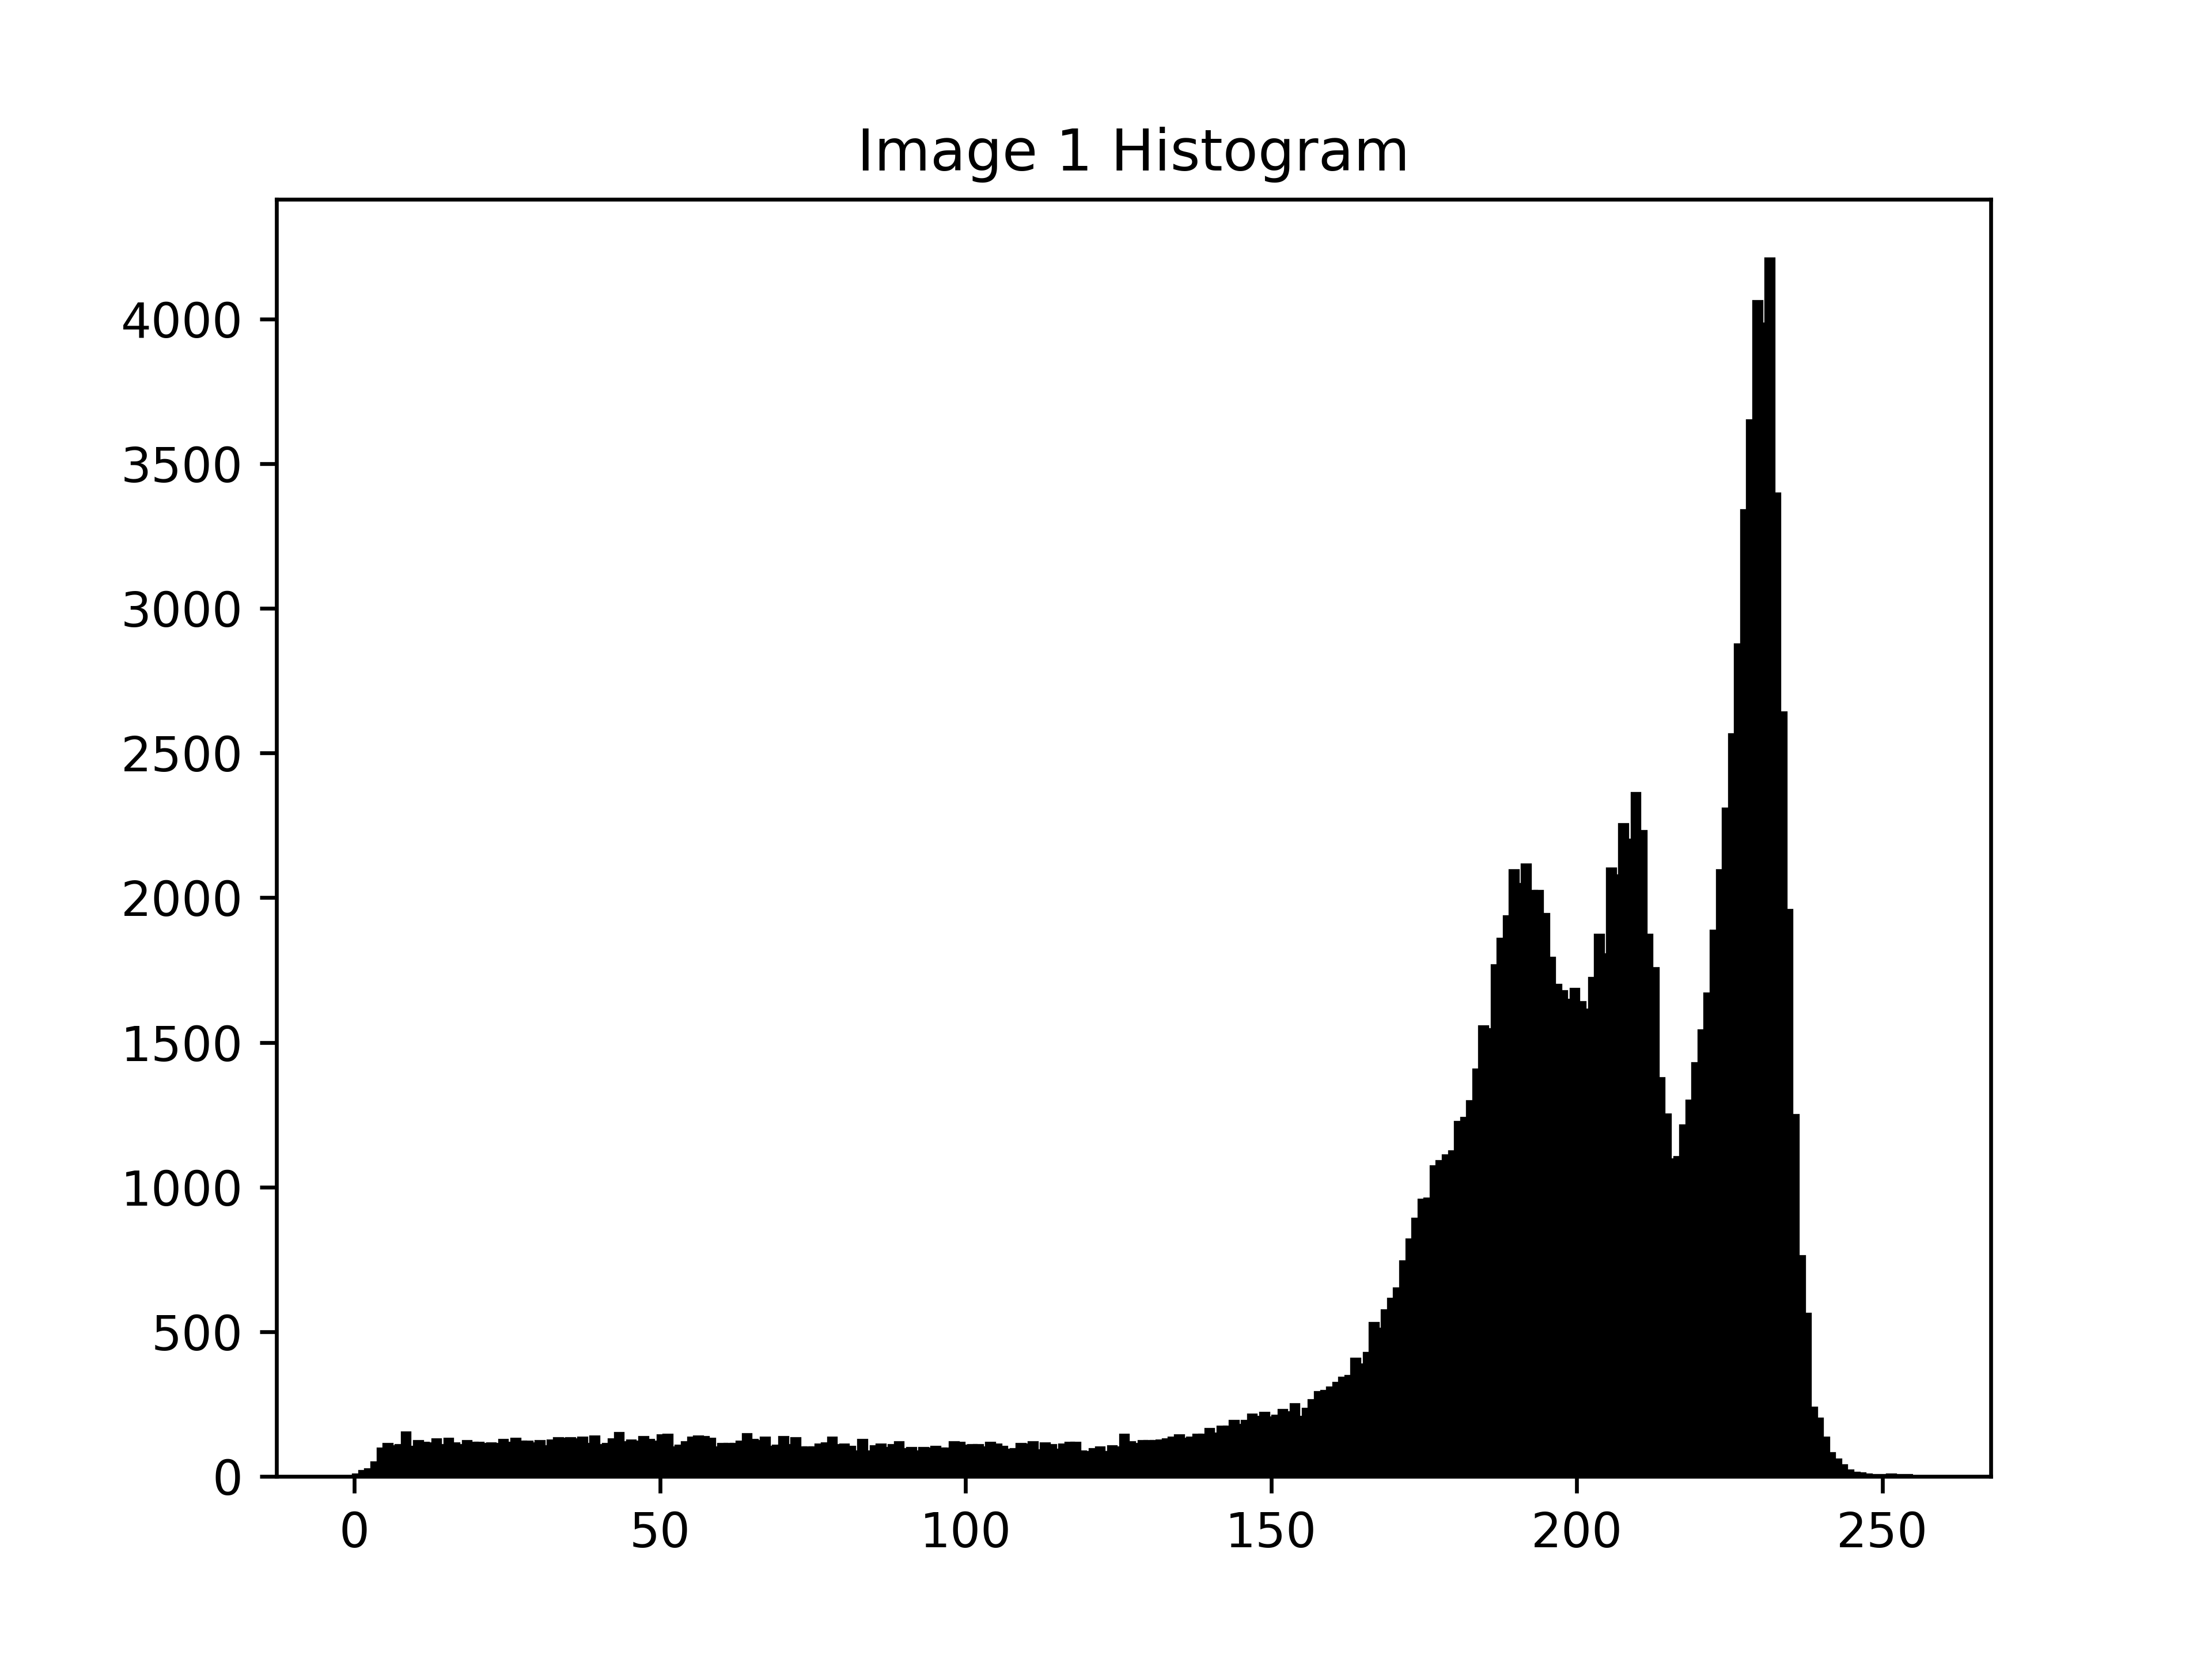
\includegraphics[width=0.32\textwidth]{img_1_hist.png}
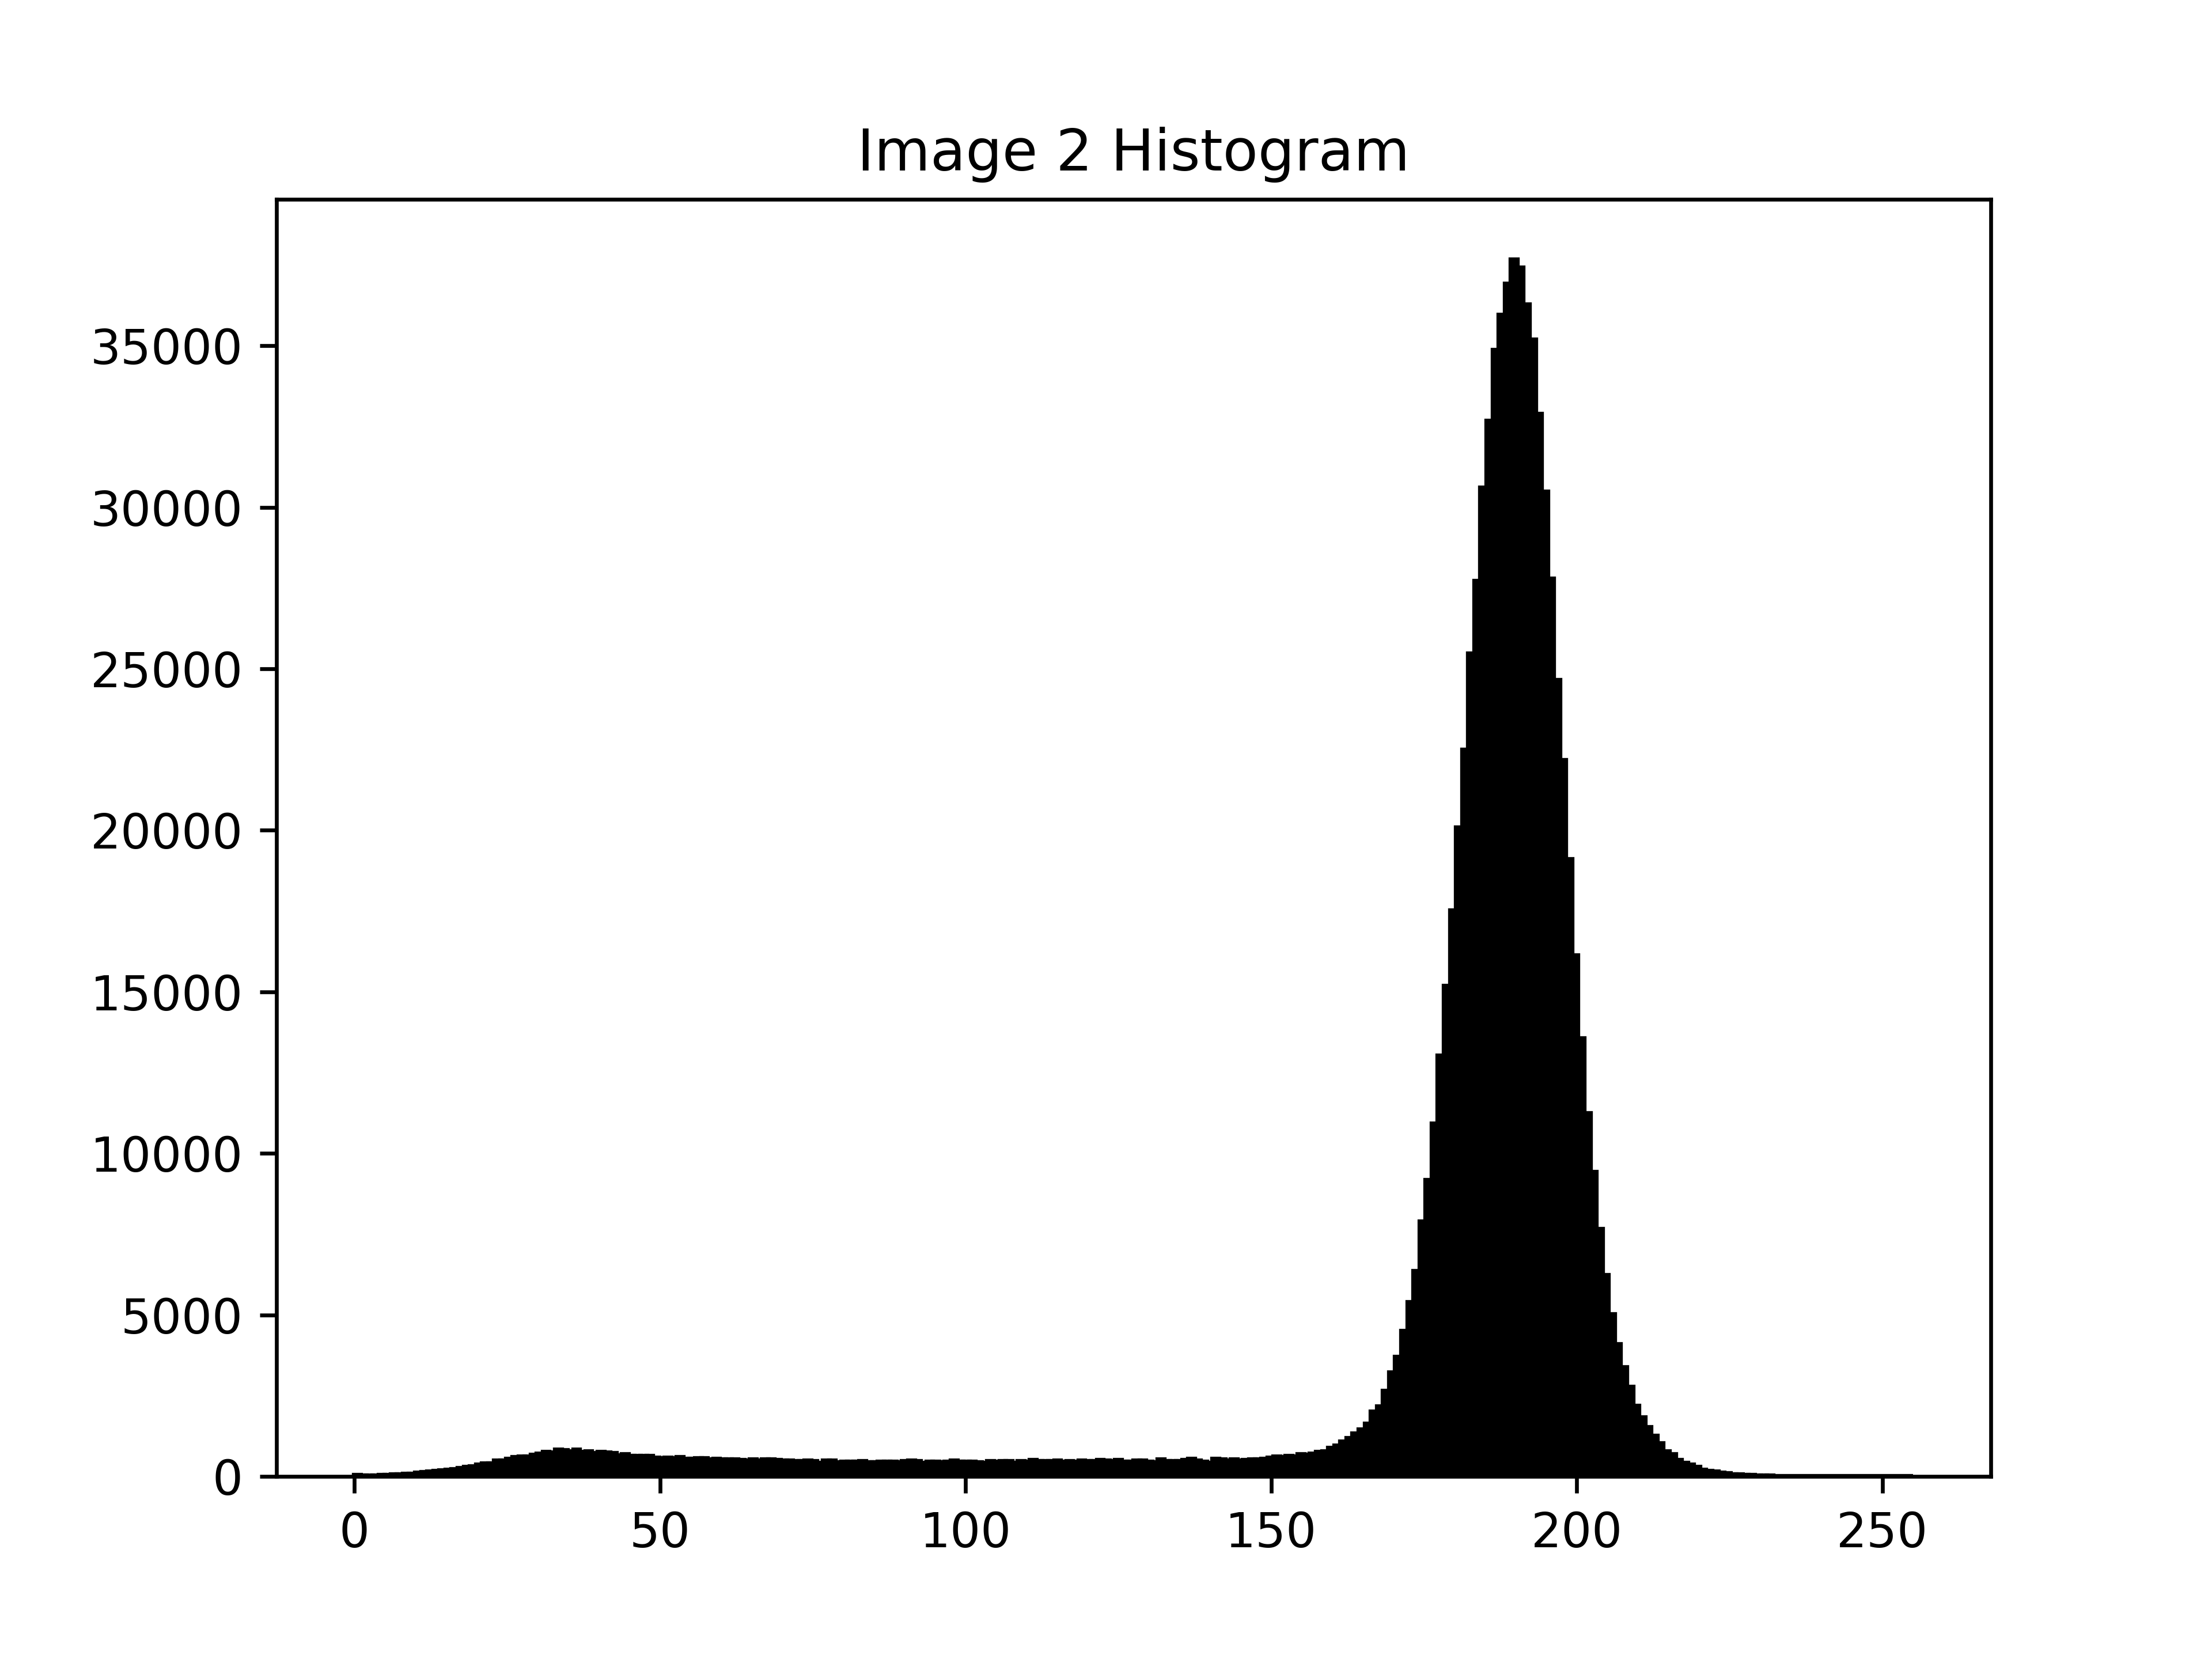
\includegraphics[width=0.32\textwidth]{img_2_hist.png}
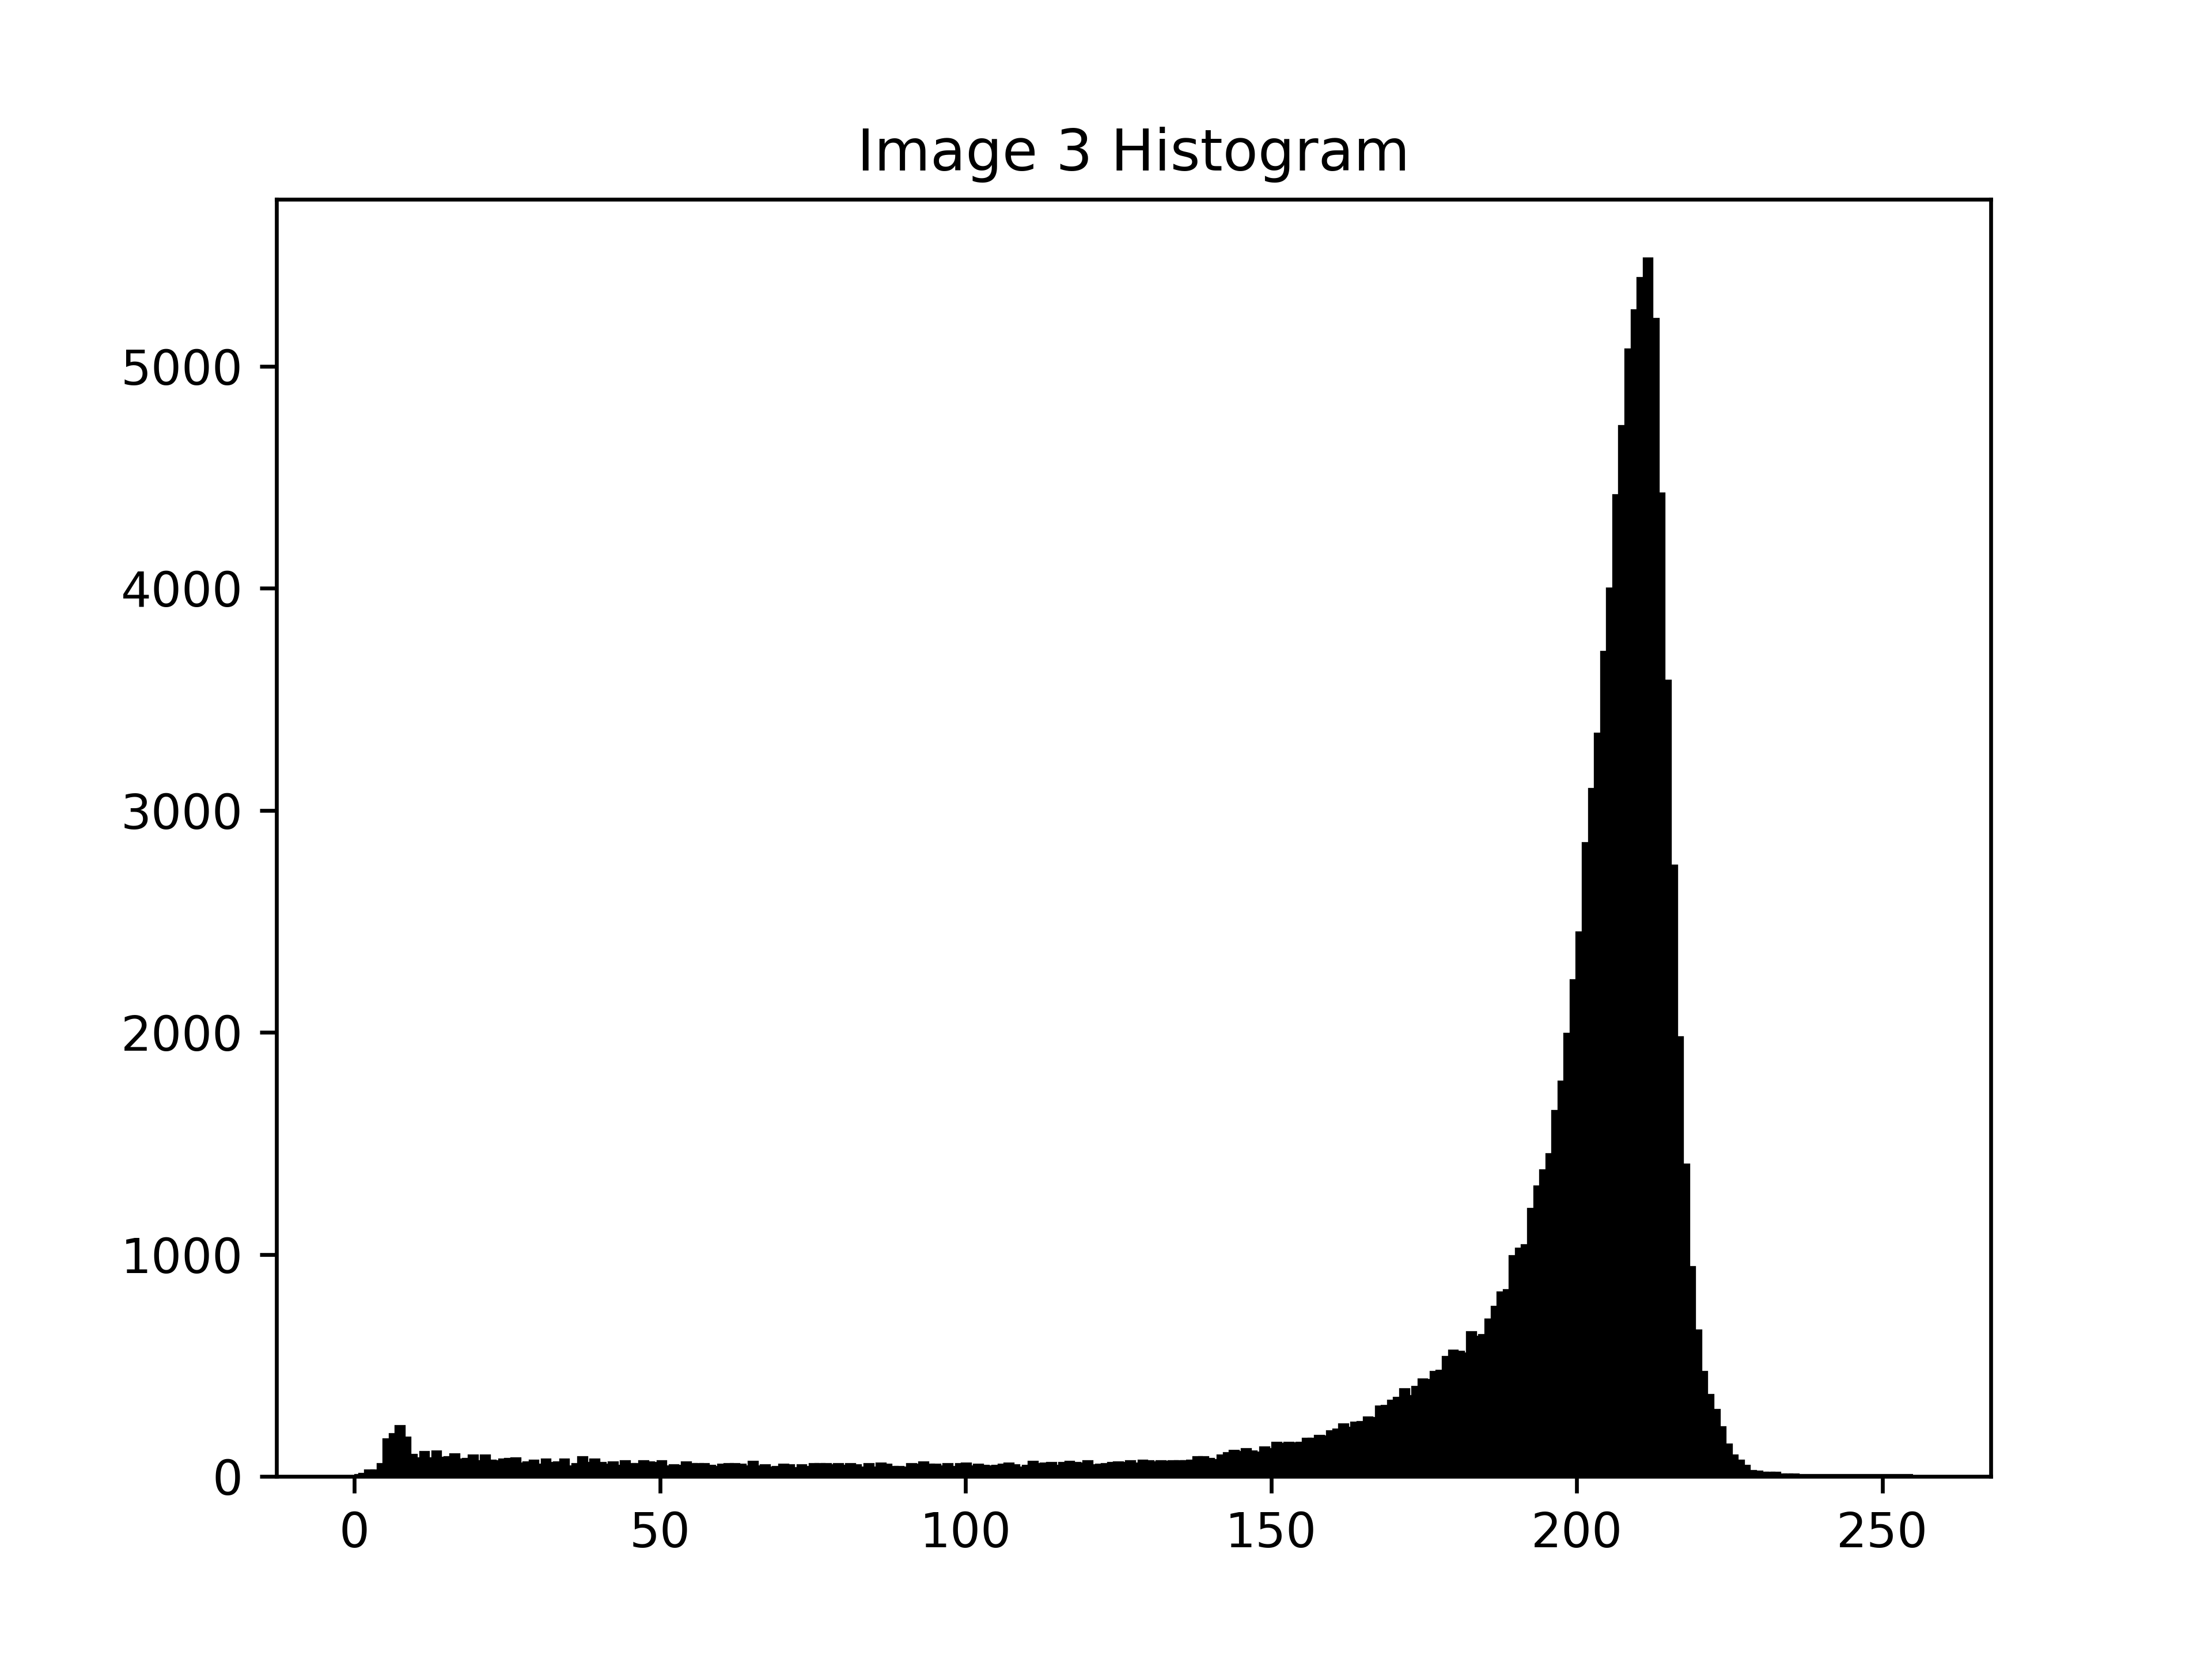
\includegraphics[width=0.32\textwidth]{img_3_hist.png}
\end{center}

\begin{listing}
\begin{verbatim}
# Image 1, 2, 3
im_final = pp.n_bit_plane_slice(im_original_gray, 1) // 1-bit slicing
\end{verbatim}
\centering
\caption{List 1: Setting For Image 1, 2, 3}
\newline
\end{listing}

\begin{listing}
\begin{verbatim}
def n_bit_plane_slice(im_np, b=1):
    new_im = np.zeros(im_np.shape)
    im_height, im_width = im_np.shape
    for x in range(im_height):
        for y in range(im_width):
            i_n = im_np[x, y] // (2 ** (8 - b))
            i_n_1 = im_np[x, y] // (2 ** (9 - b))
            new_im[x, y] = (i_n - i_n_1 * 2) * 255
    return new_im.astype(np.uint8)
\end{verbatim}
\centering
\caption{List 2: N-Bit Slicing}
\newline
\end{listing}

\begin{center}
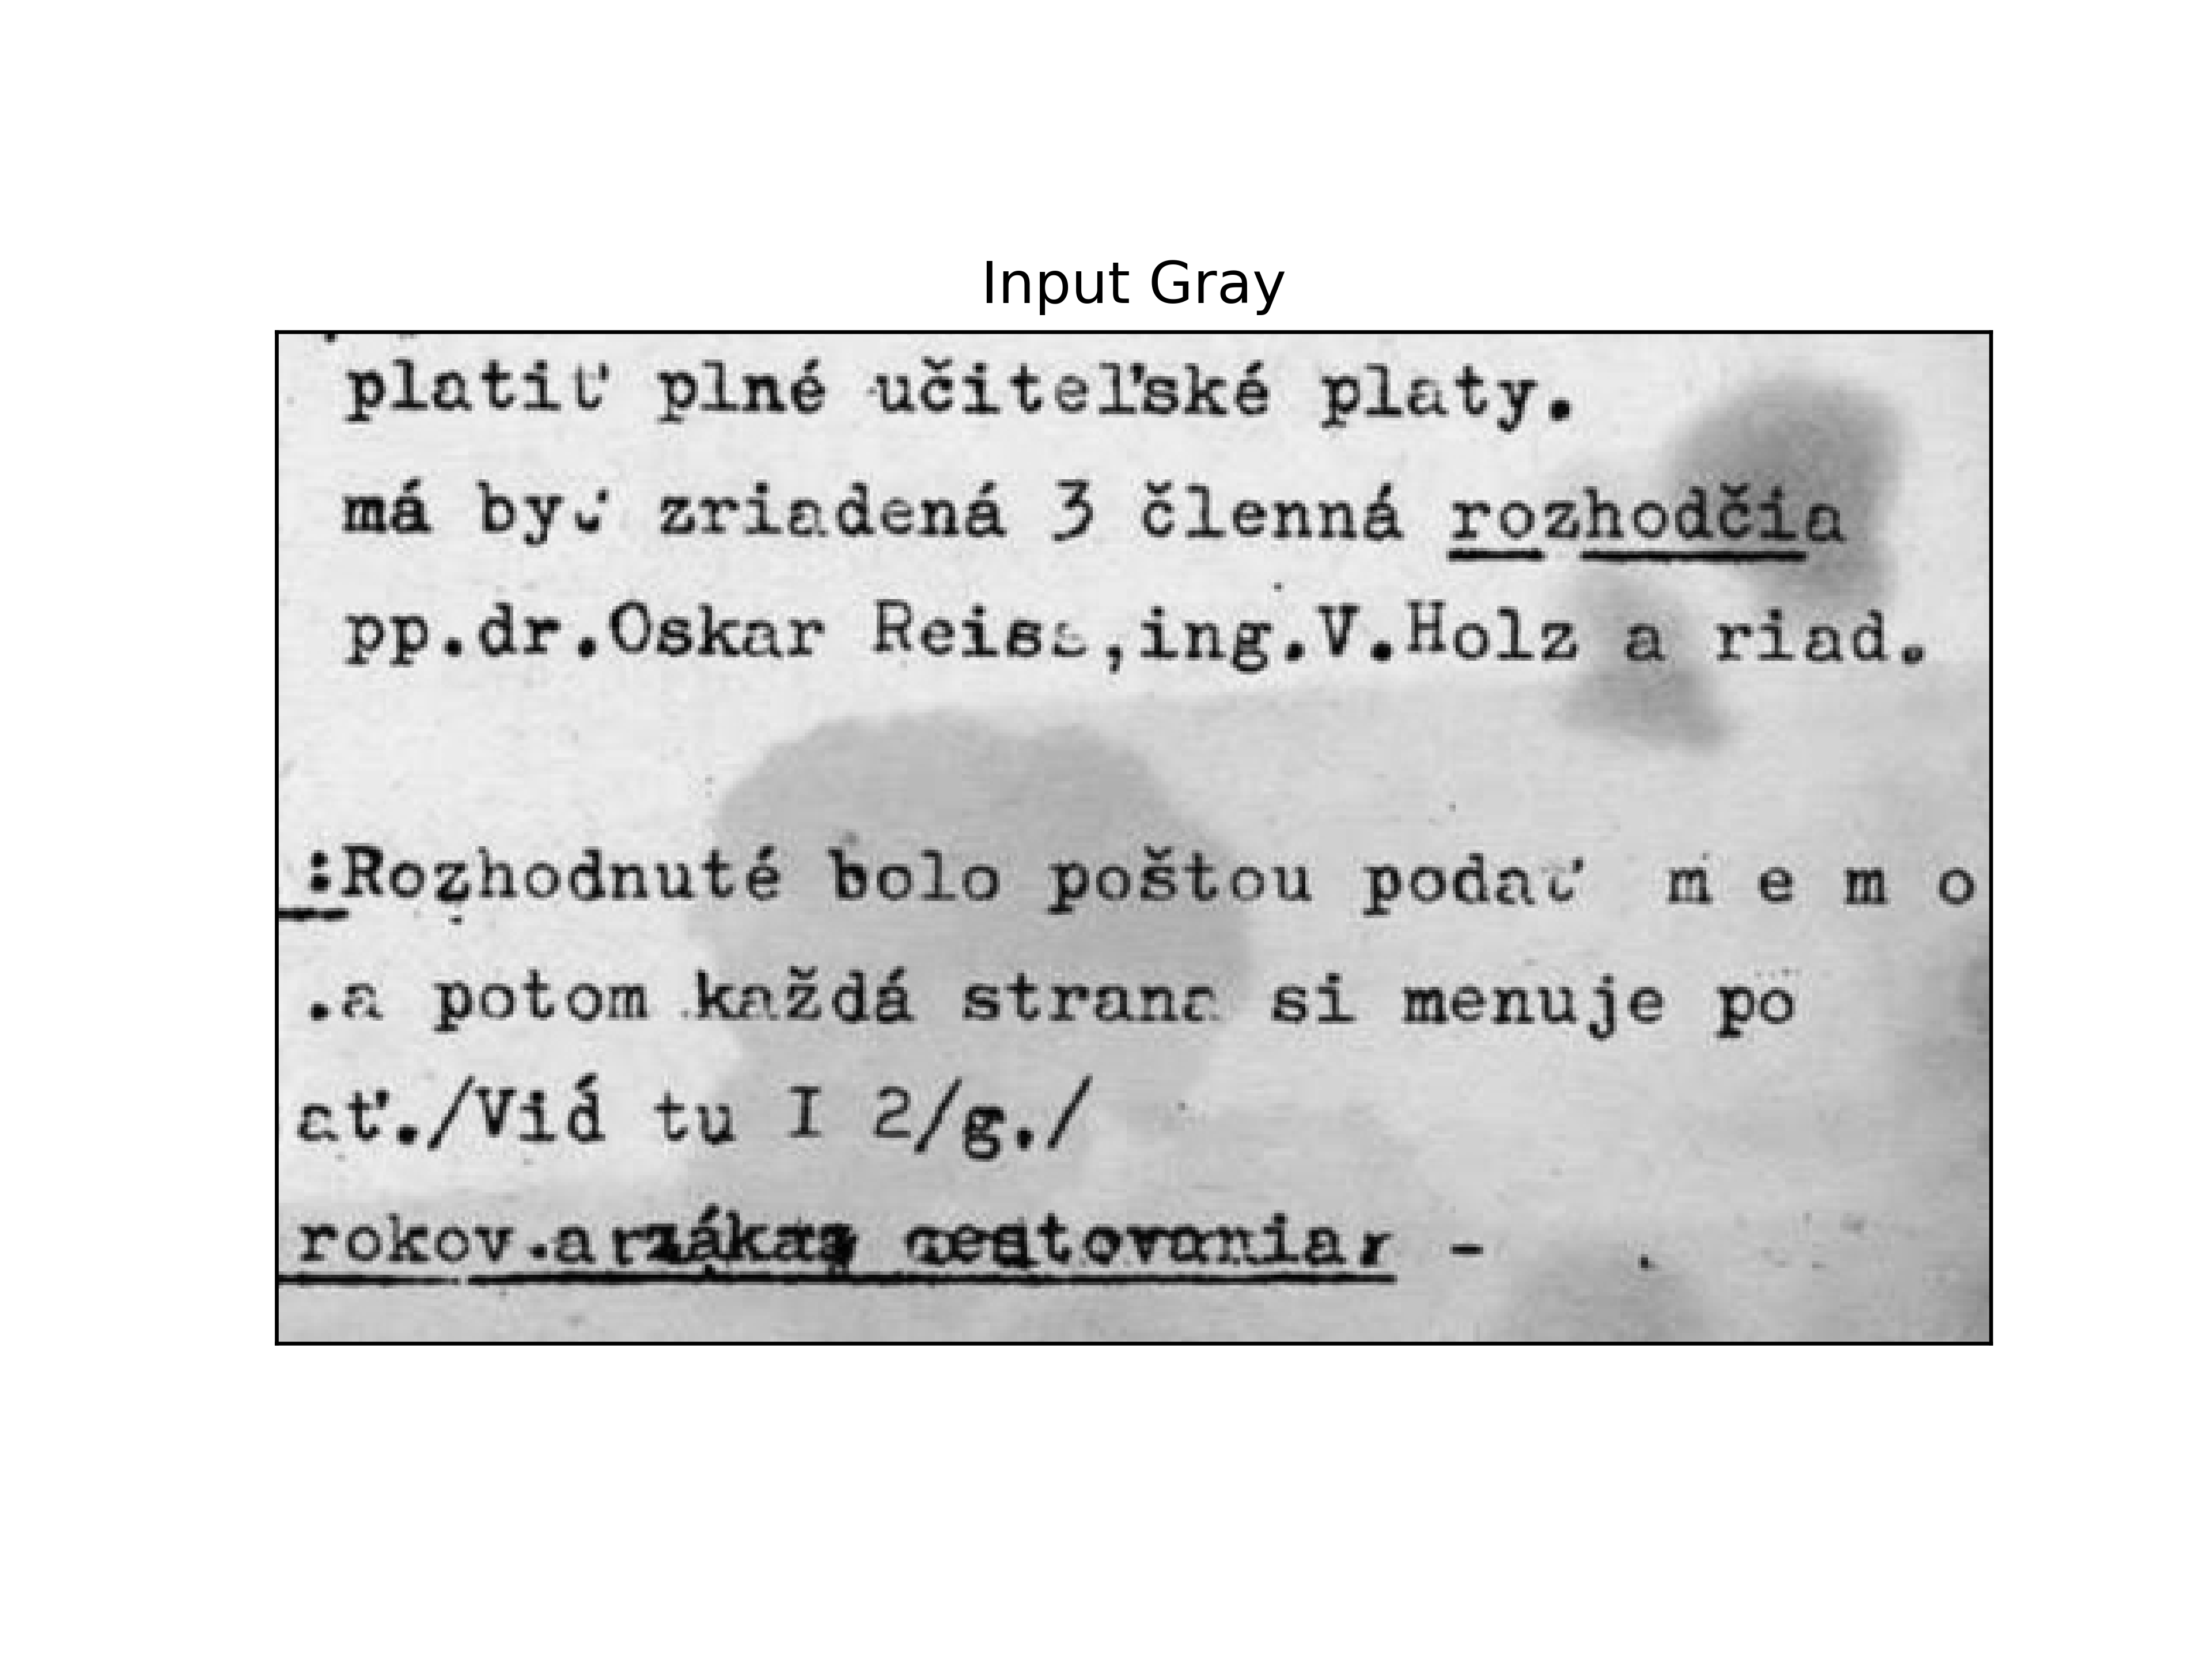
\includegraphics[width=0.49\textwidth]{img_1_gray.png}
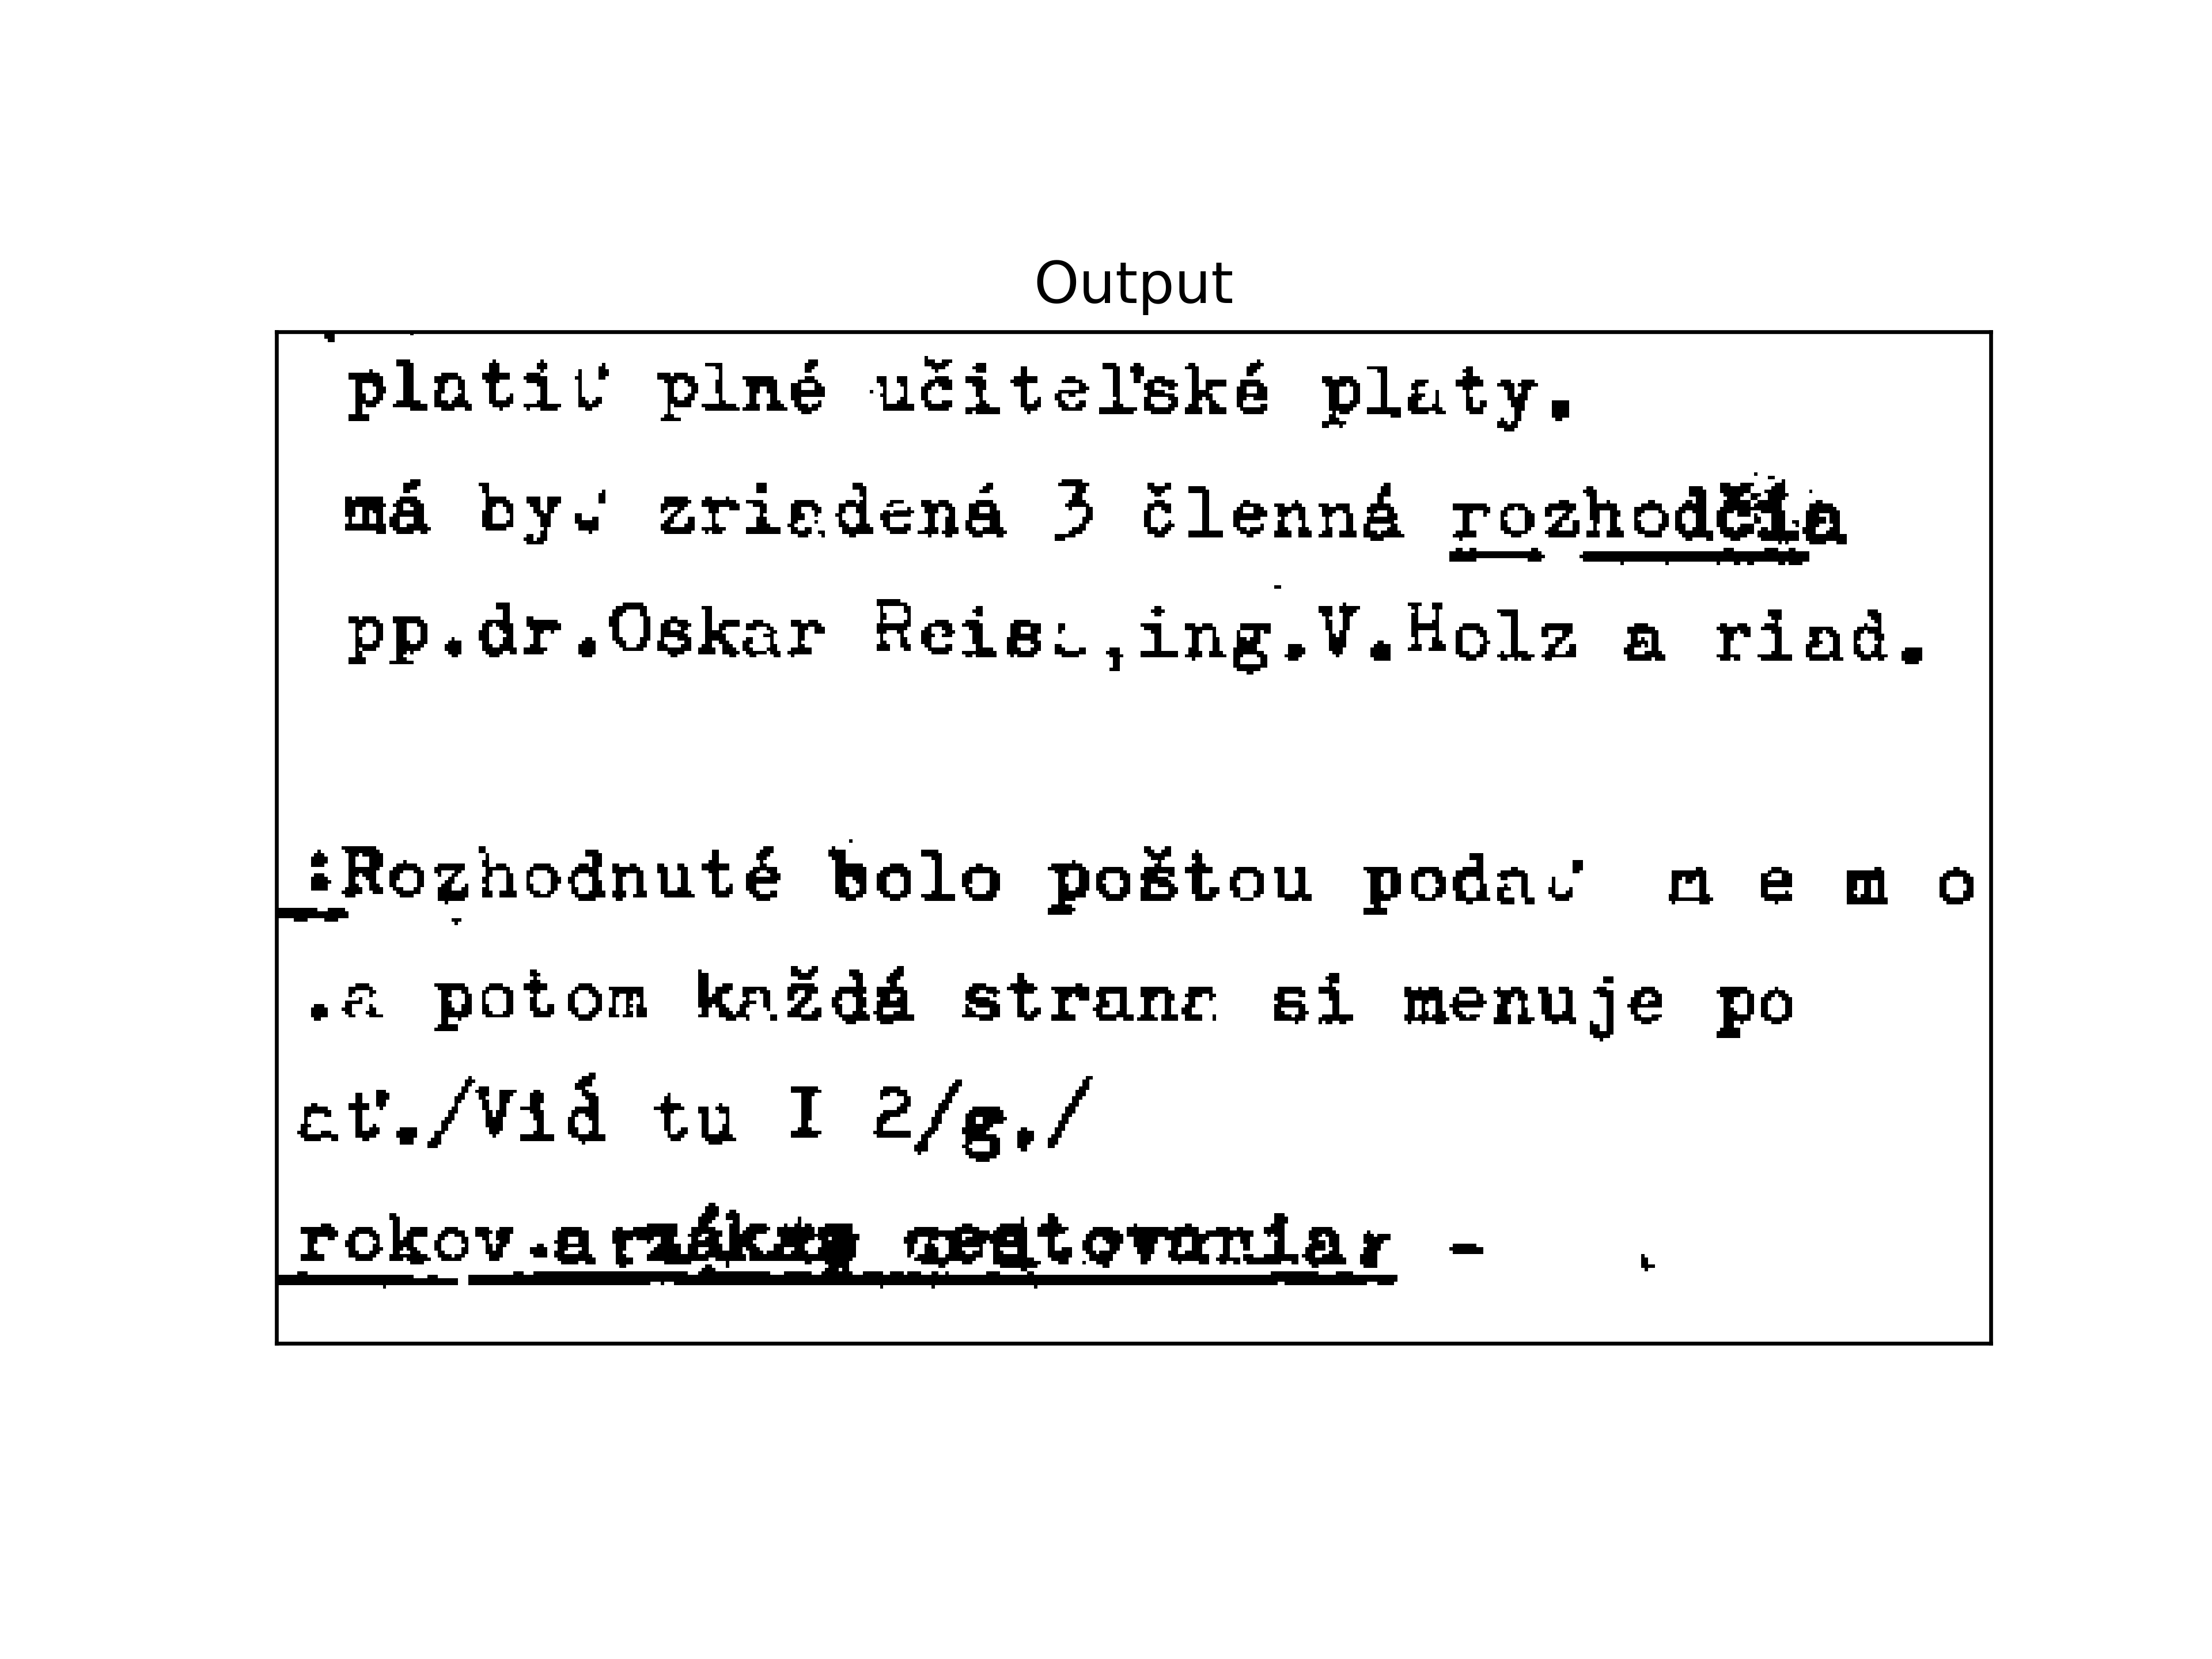
\includegraphics[width=0.49\textwidth]{img_1_output.png}
\end{center}

\begin{center}
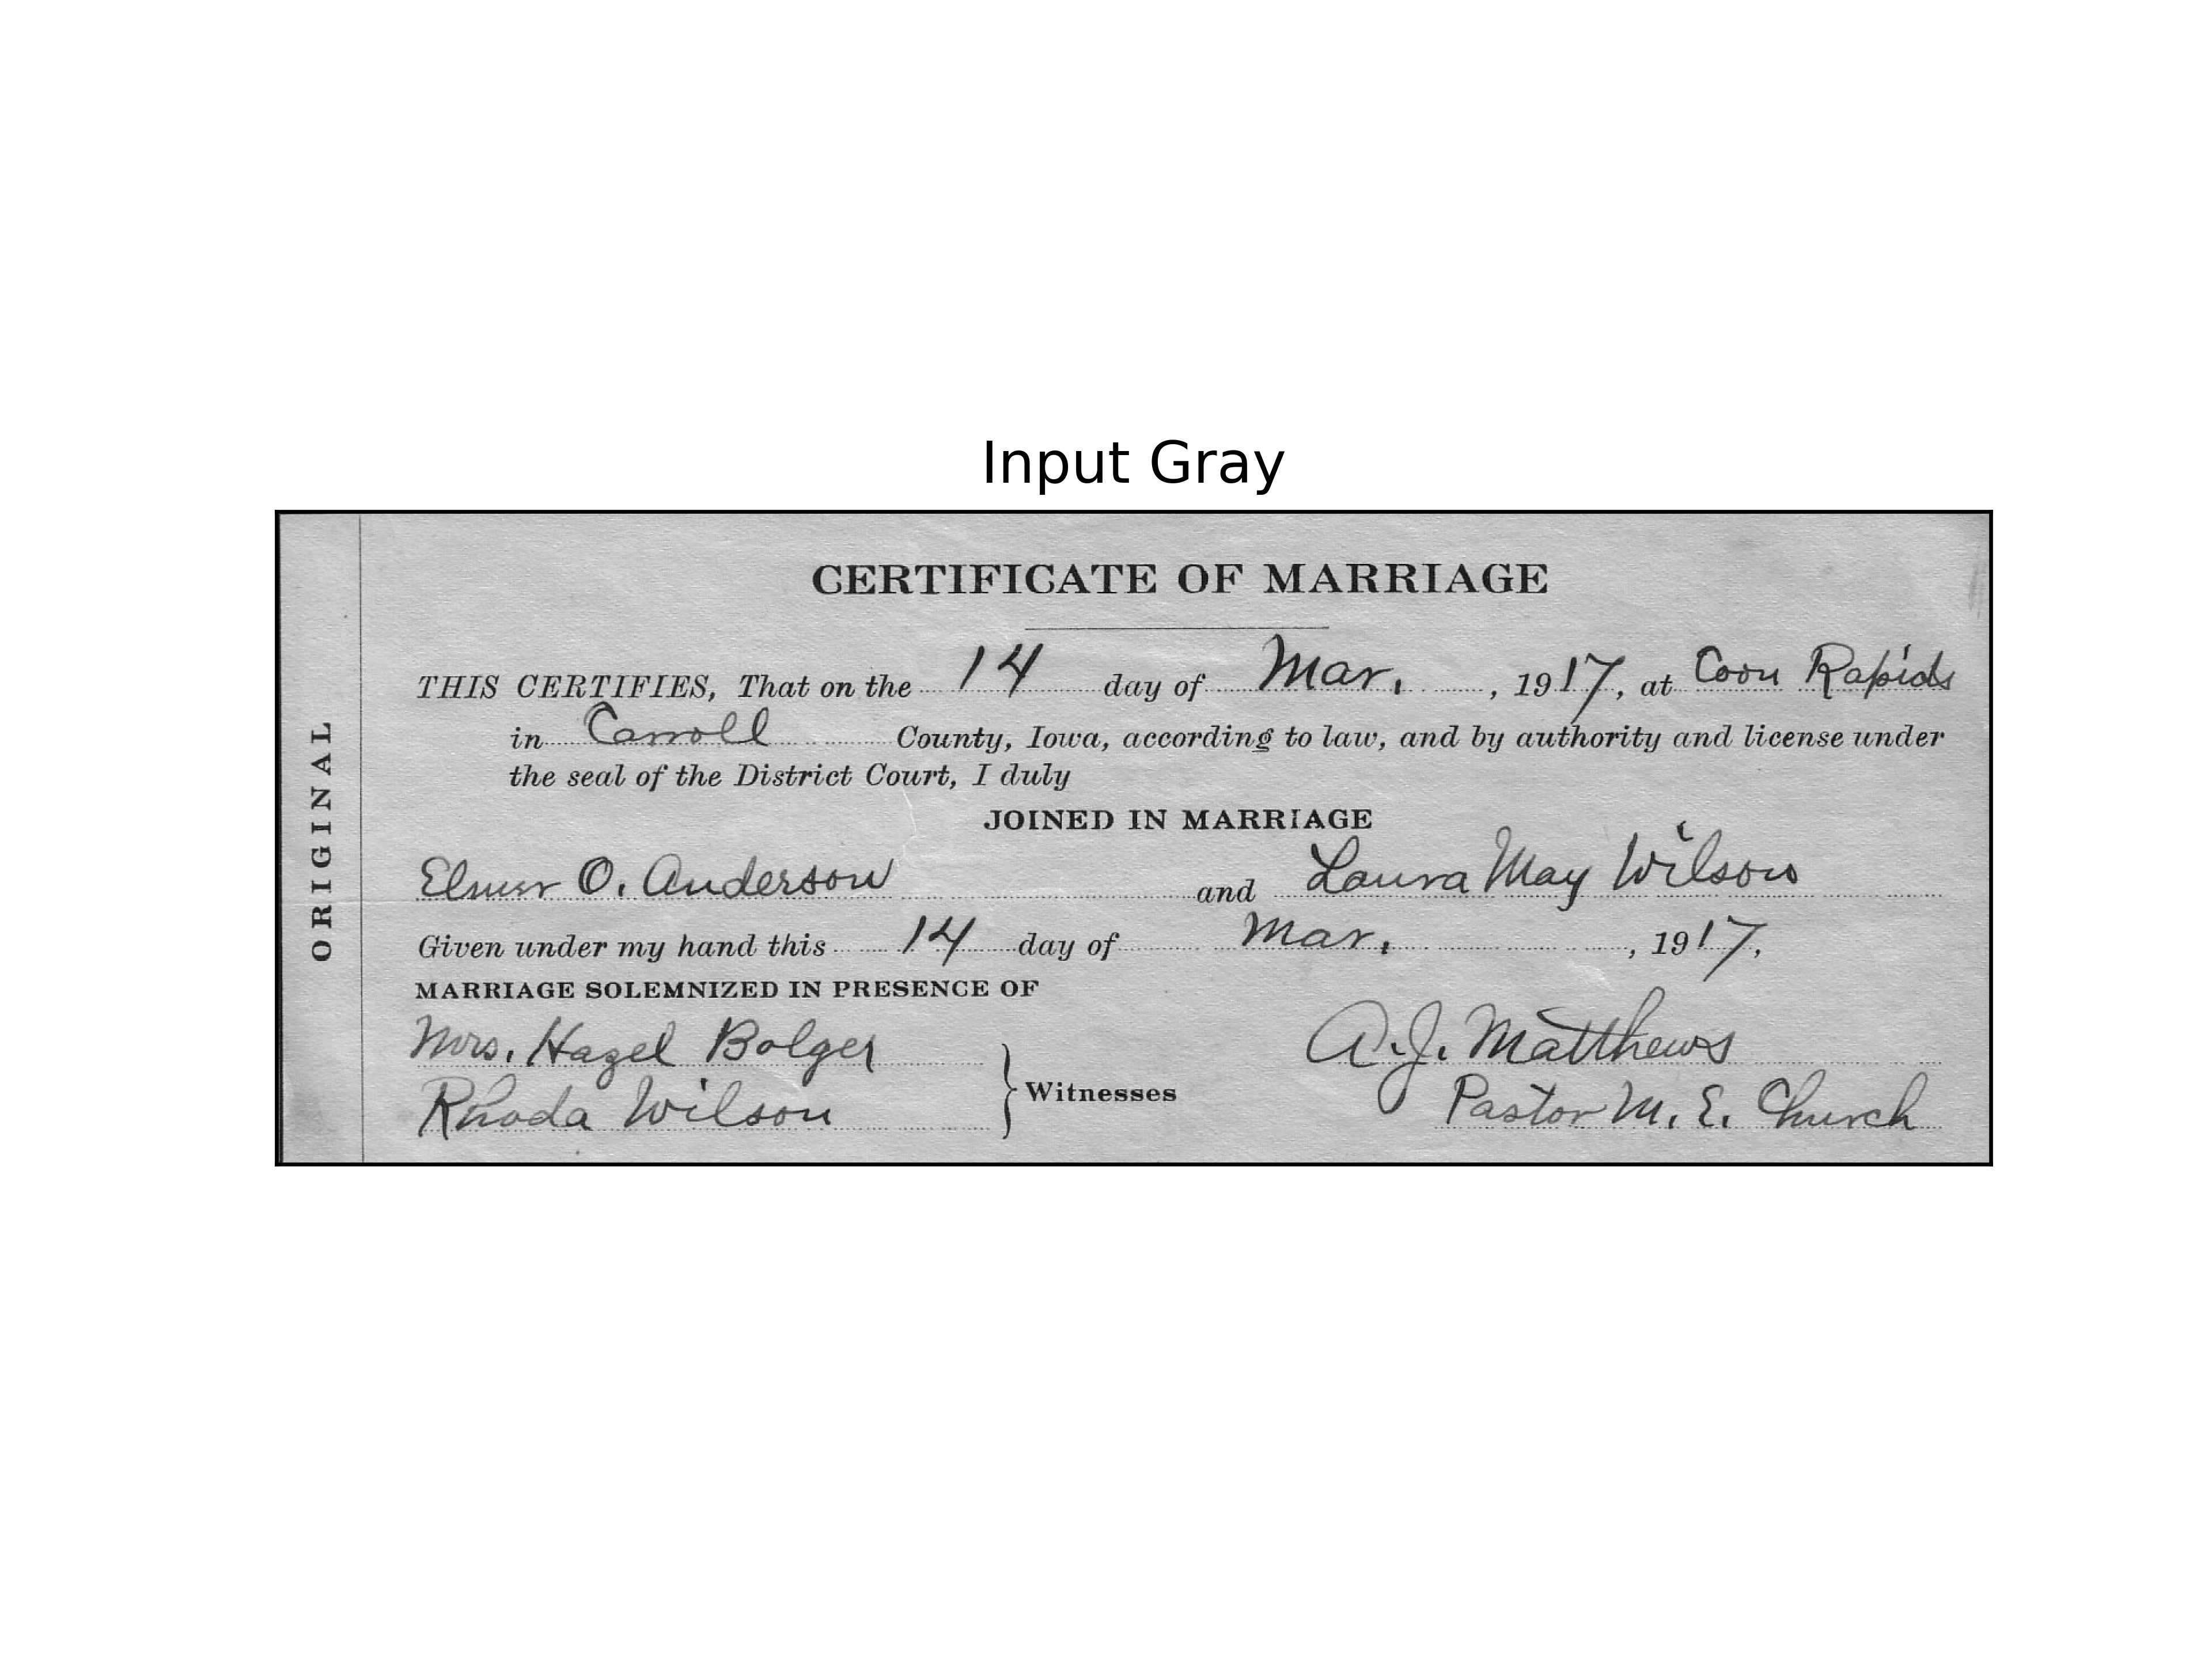
\includegraphics[width=0.49\textwidth]{img_2_gray.png}
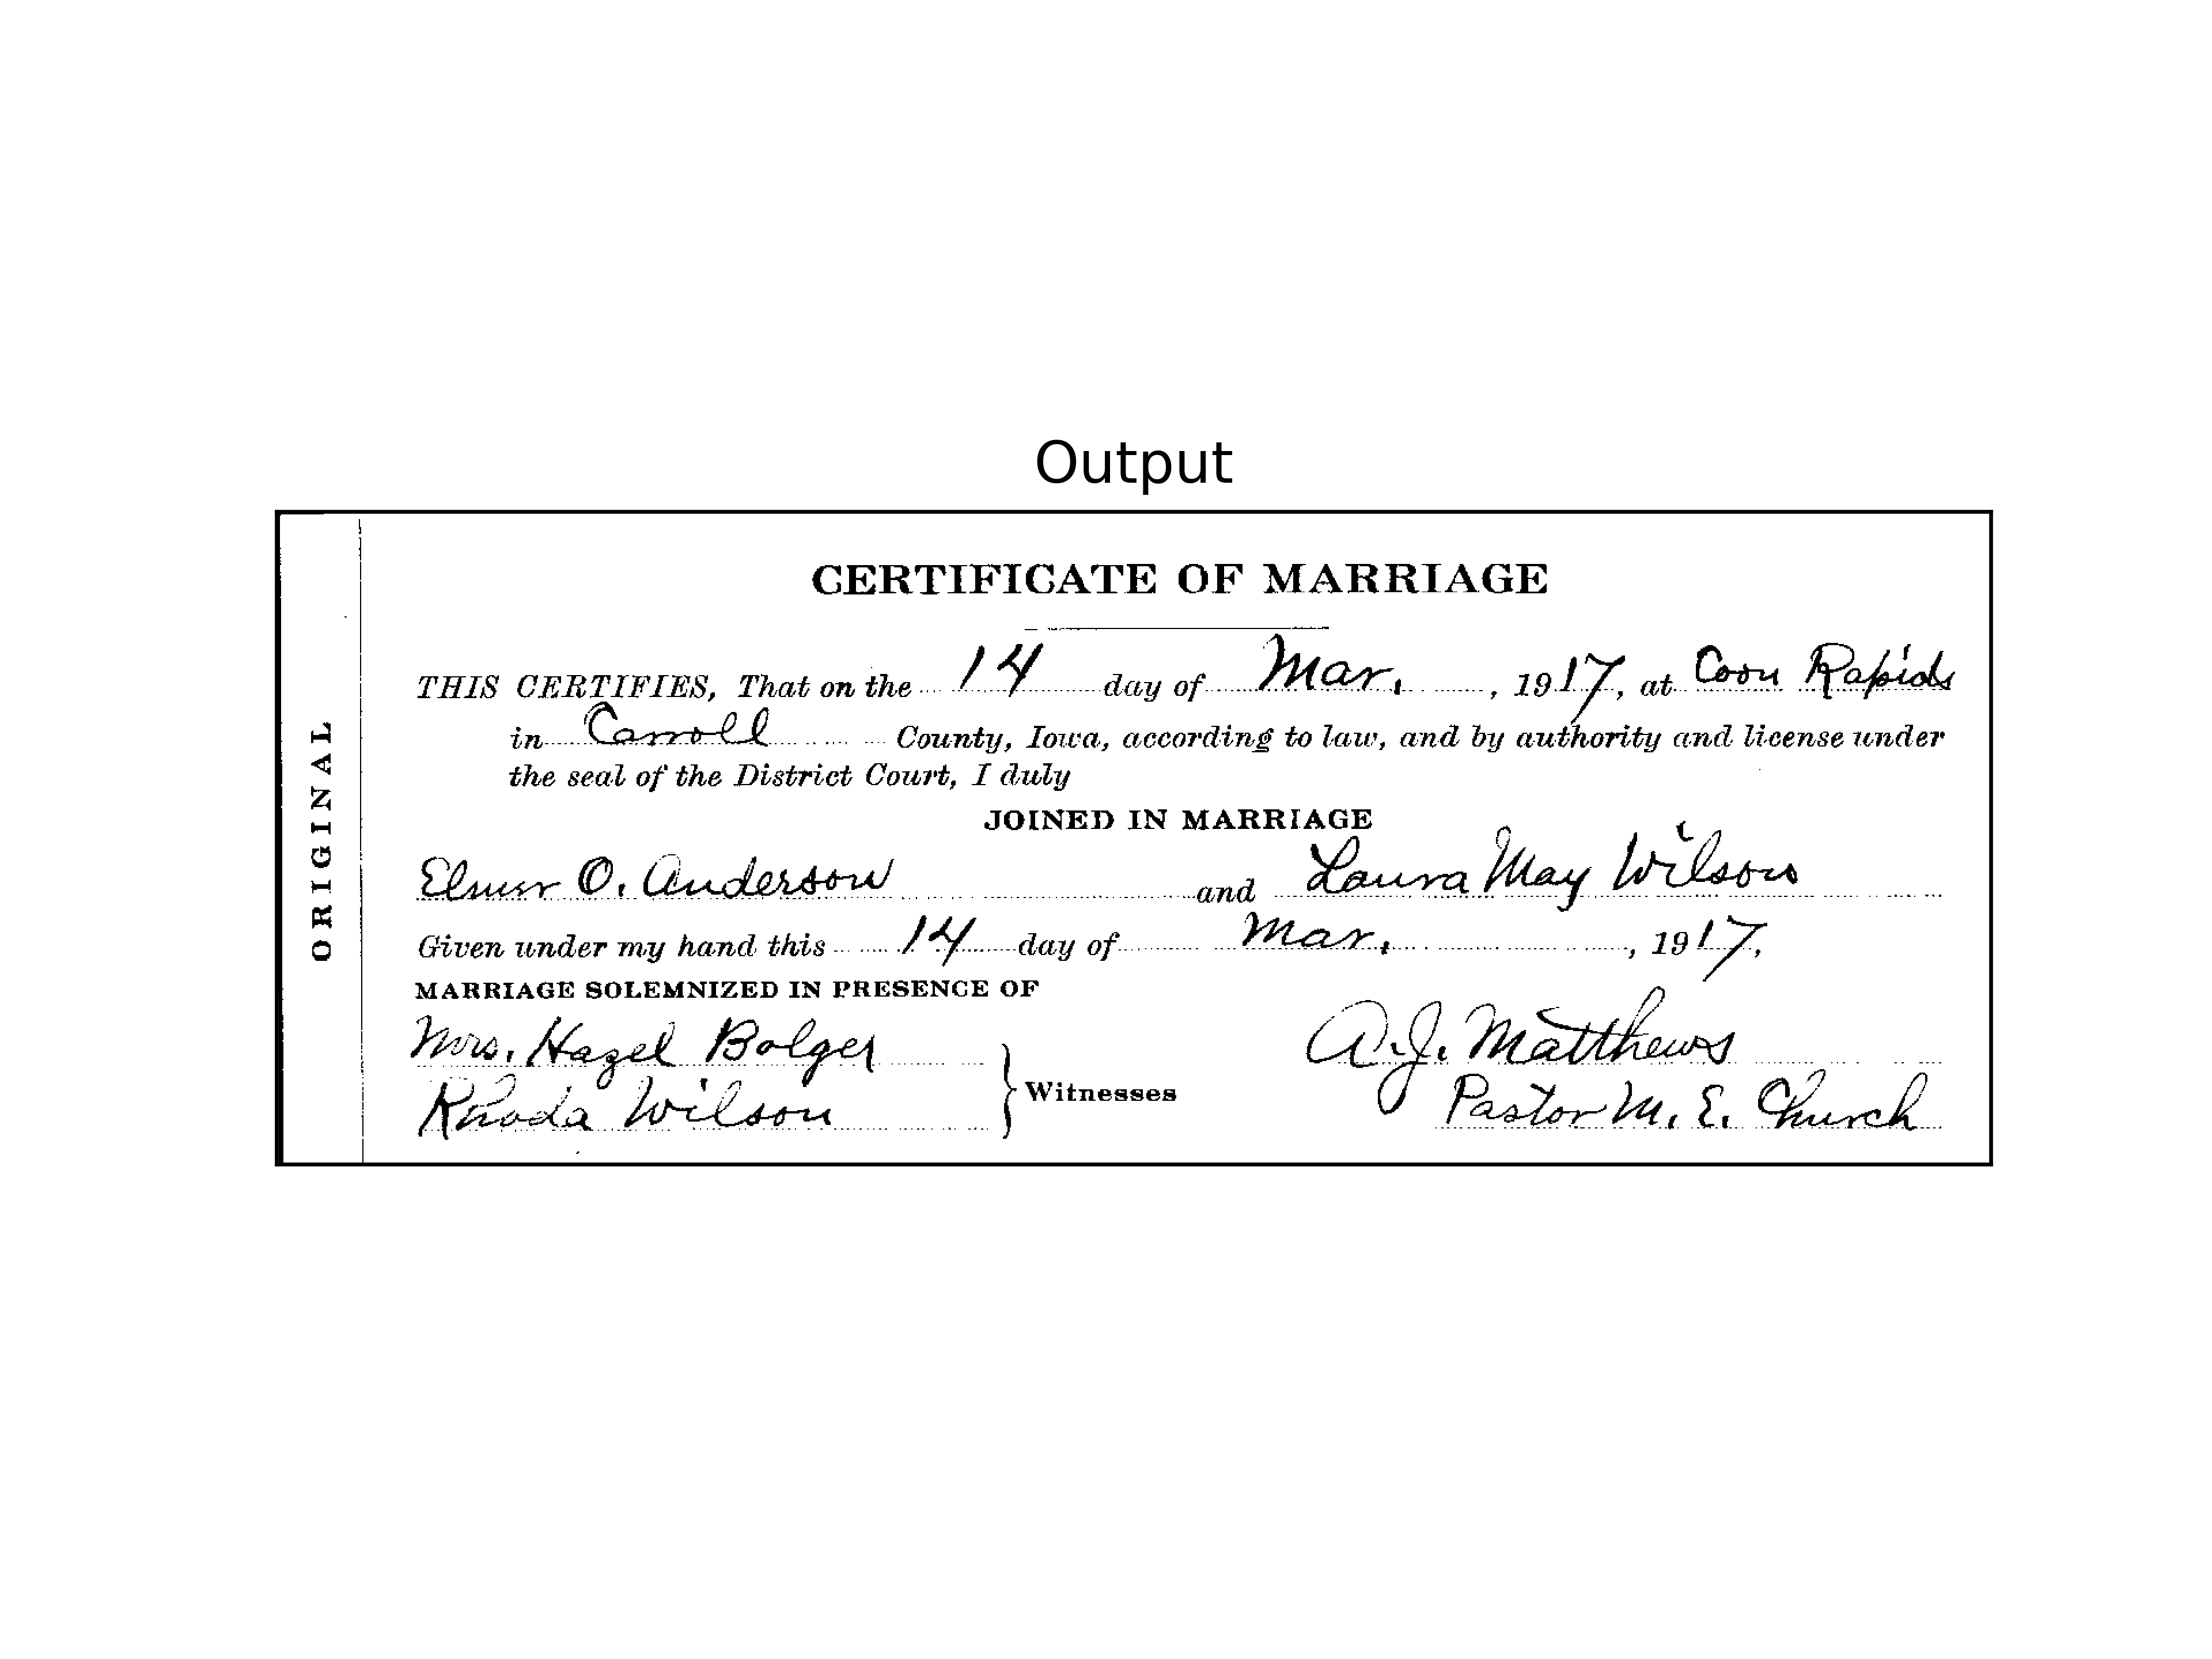
\includegraphics[width=0.49\textwidth]{img_2_output.png}
\end{center}

\begin{center}
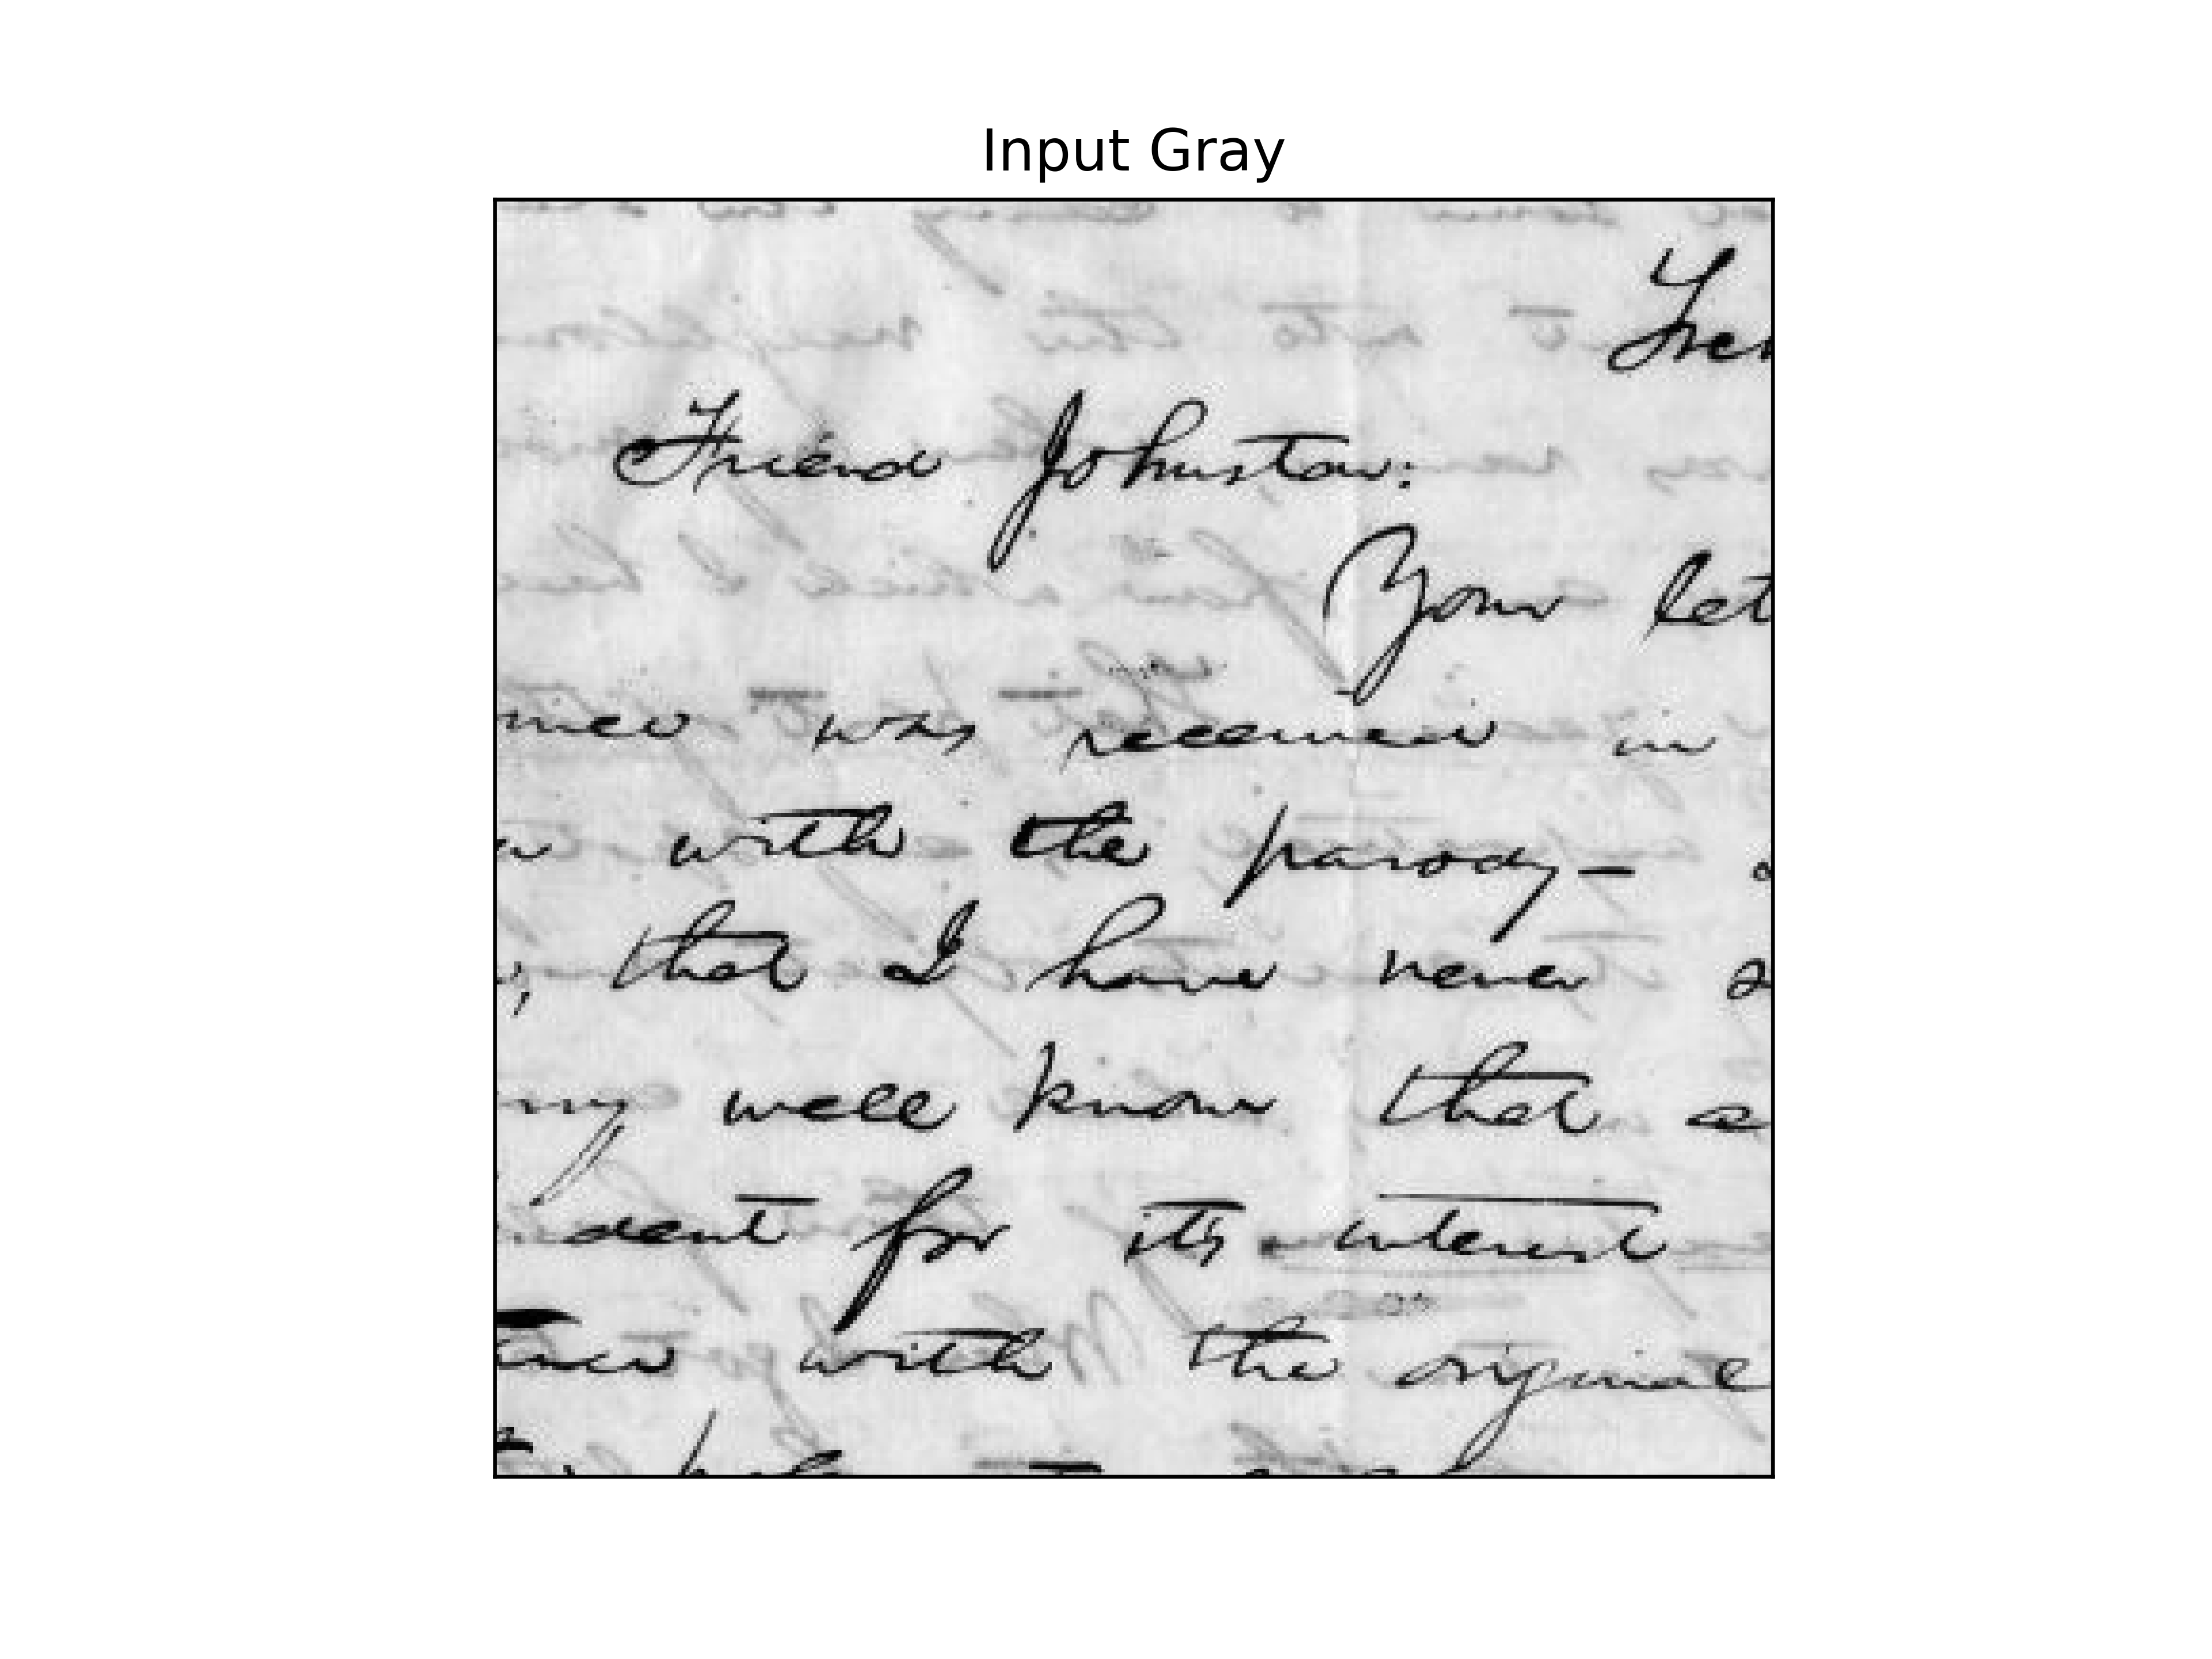
\includegraphics[width=0.49\textwidth]{img_3_gray.png}
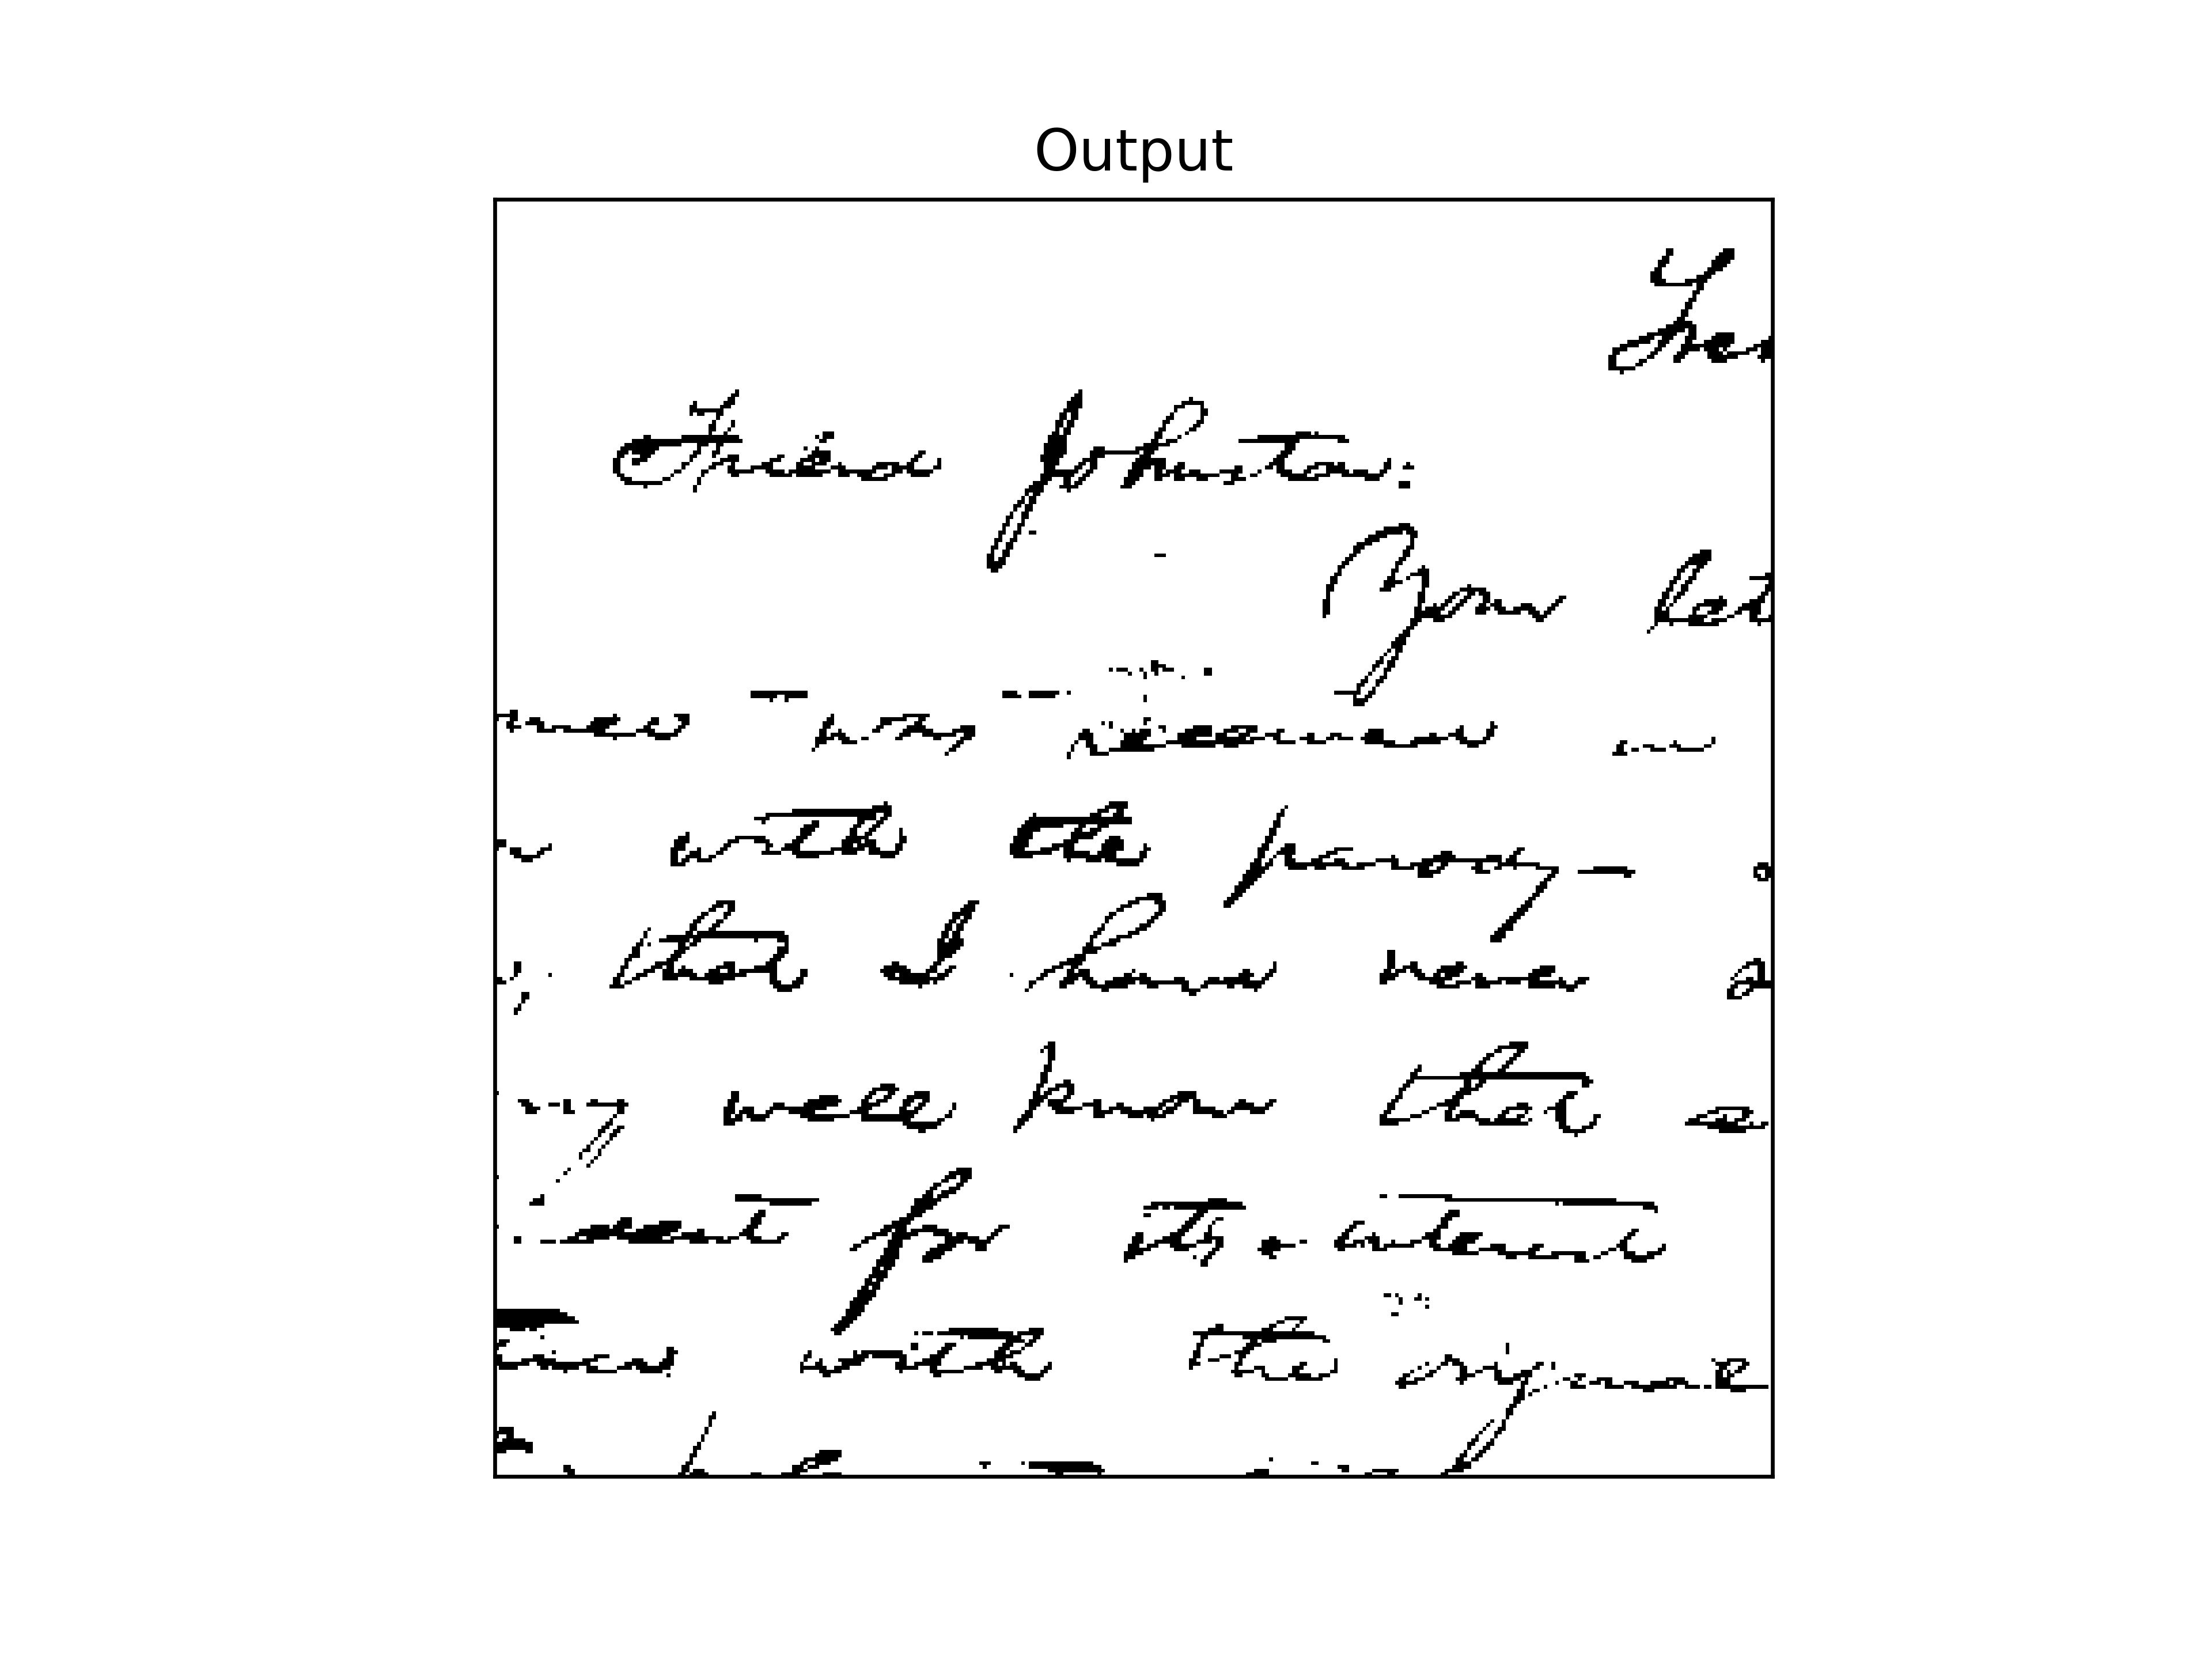
\includegraphics[width=0.49\textwidth]{img_3_output.png}
\end{center}

Image 4 and 5 have strong shadow on them, hence it becomes difficult for
global threshold. However a local threshold using Otsu's method can improve
the processed image's quality significantly. Before applying threshold,
alpha-trimmed mean filter is used to remove noise and smooth the image. The
local Otsu's threshold method is from the 'skimage.filters.rank' library. As
shown in the list below, the 'rad' variable specifies the radius of a
disk-like window for local Otsu's threshold. 

From the picture it can be noticed that one problem of this local Otsu's
threshold is the black spot on the background, which is mainly due to the
uneven illumination on the image. This problem can be partly eliminated by
enlarging the window size, however, this decreases the text resolution also.
In image 9, this problem is solved by applying a line mask. Unfortunately, the
it does not work for Image 4 and 5, which have much strong shadow on it.

\begin{listing}
\begin{verbatim}
# Image 4, 5 
im_step_1 = alpha_trimmed_mean(im_original_gray, window_size=3, alpha=2)
im_final = otsu_threshold(im_step_1.astype(np.uint8), 100)
\end{verbatim}
\centering
\caption{List 3: Setting For Image 4, 5}
\newline
\end{listing}

\begin{listing}
\begin{verbatim}
def alpha_trimmed_mean(im_np, window_size=3, alpha=2):
    pad_length = window_size // 2
    im_np_pad = np.pad(im_np, (pad_length,), 'edge')
    im_height, im_width = np.shape(im_np_pad)
    im_new = np.zeros(np.shape(im_np))
    for m in range(pad_length, im_height - pad_length):
        for n in range(pad_length, im_width - pad_length):
            window_elements = im_np_pad[m-pad_length:m+pad_length+1, n-pad_length:n+pad_length+1]
            ordered_elements = np.sort(window_elements, axis=None)
            im_new[m-pad_length, n-pad_length] = np.mean(
                ordered_elements[int(alpha/2):int(-(alpha/2))]).astype(np.uint8)
    return im_new
\end{verbatim}
\centering
\caption{List 4: Alpha-Trimmed Mean Filtering}
\newline
\end{listing}

\begin{listing}
\begin{verbatim}
def otsu_threshold(im_np, rad):
  local_otsu = otsu(im_np, disk(rad))
  thresh_image = im_np >= local_otsu
  return np.uint8(thresh_image*255)
\end{verbatim}
\centering
\caption{List 5: Local Otsu's Threshold}
\newline
\end{listing}

\begin{center}
\includegraphics[width=0.32\textwidth]{img_4_gray.png}
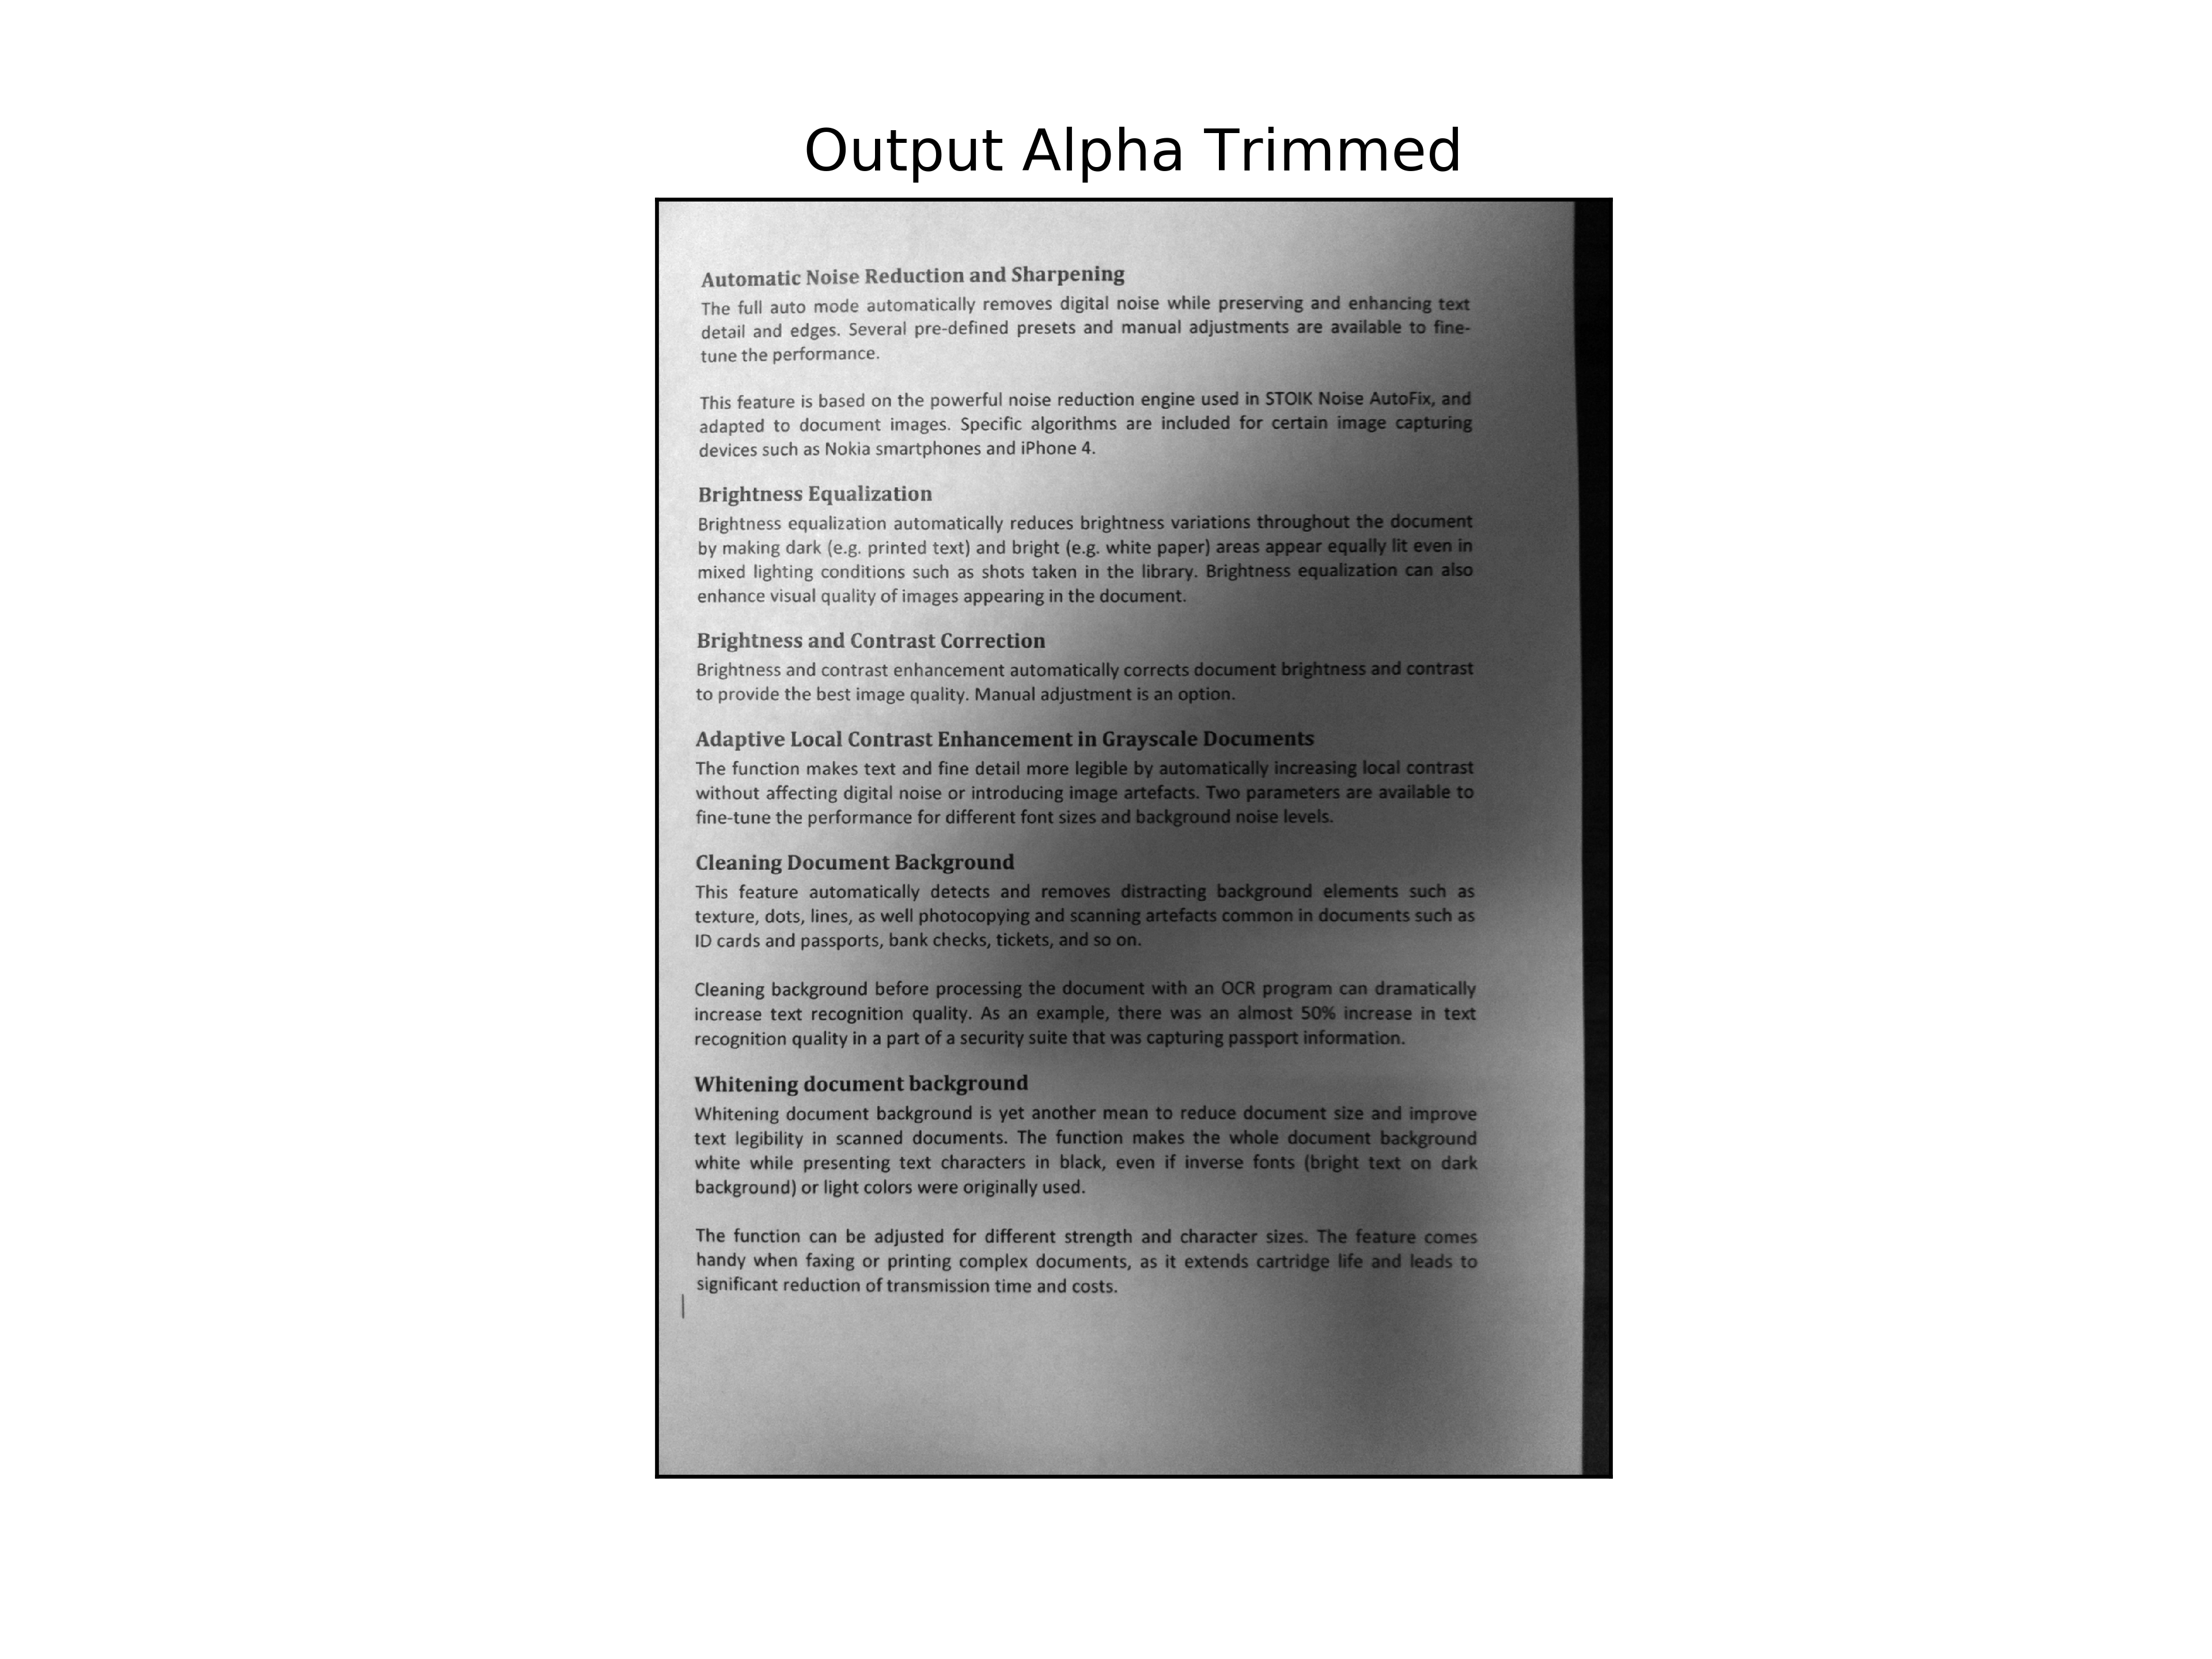
\includegraphics[width=0.32\textwidth]{img_4_output_alpha_trimmed.png}
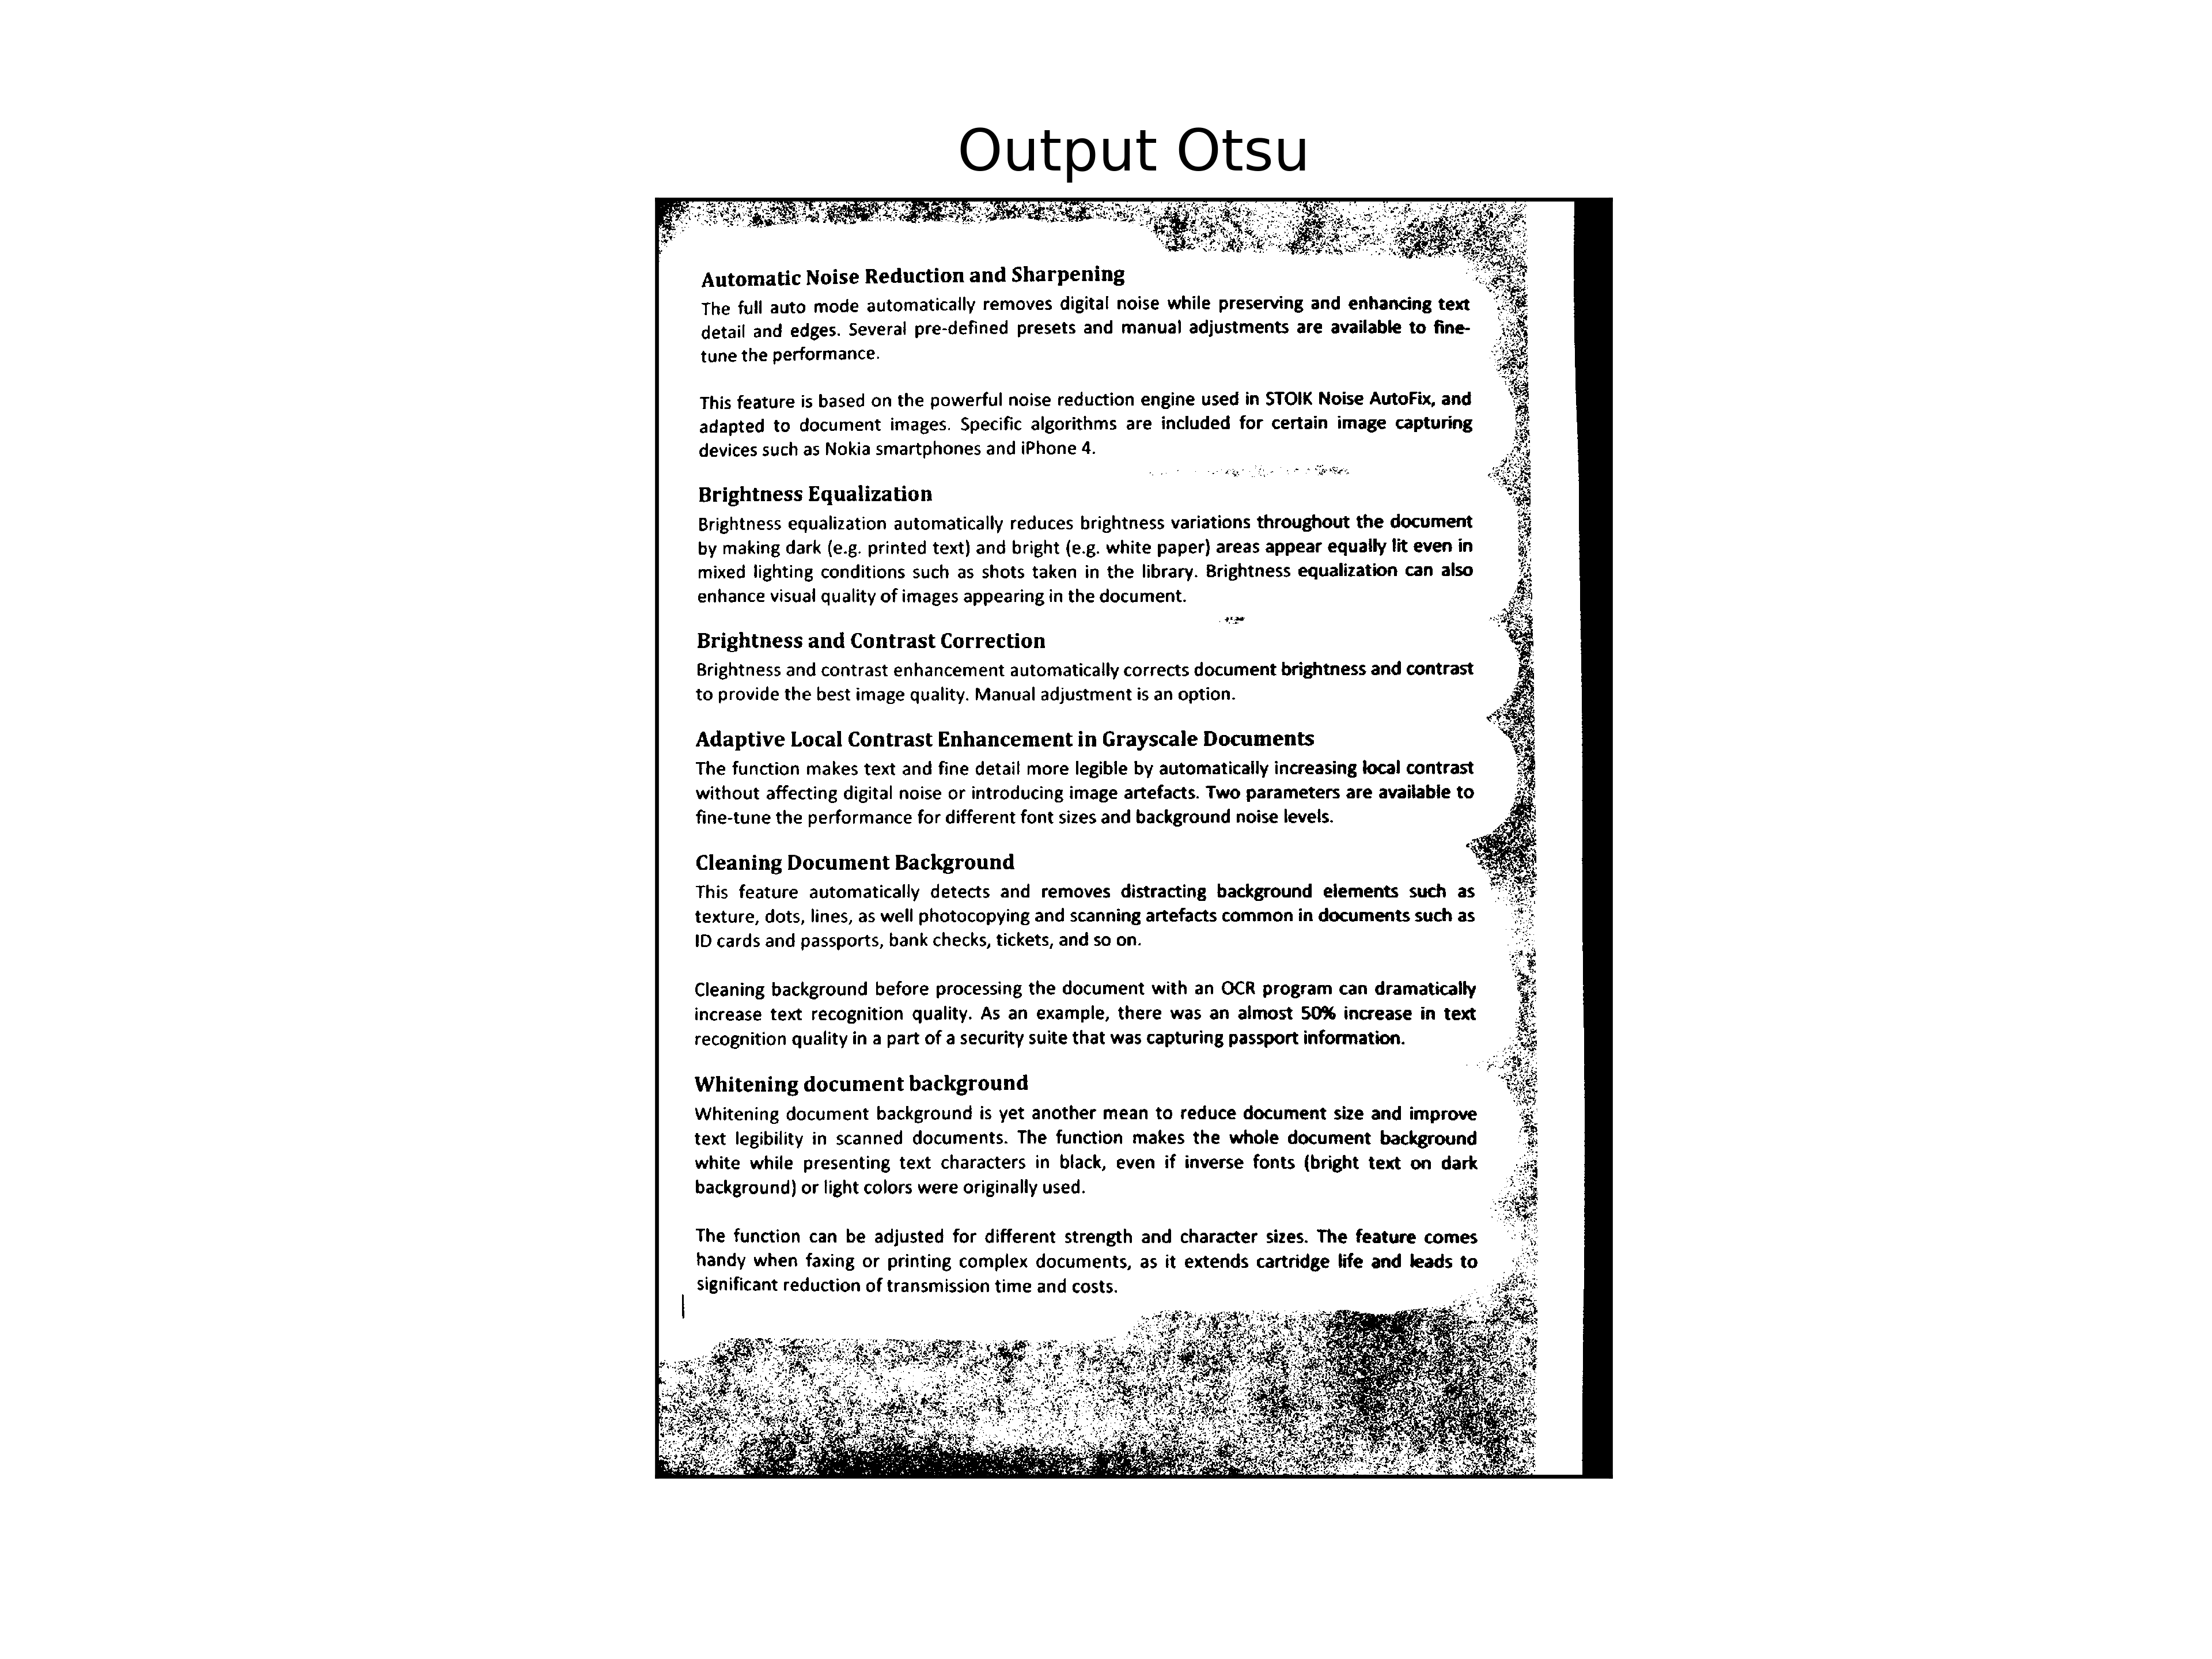
\includegraphics[width=0.32\textwidth]{img_4_output_otsu.png}
\end{center}

\begin{center}
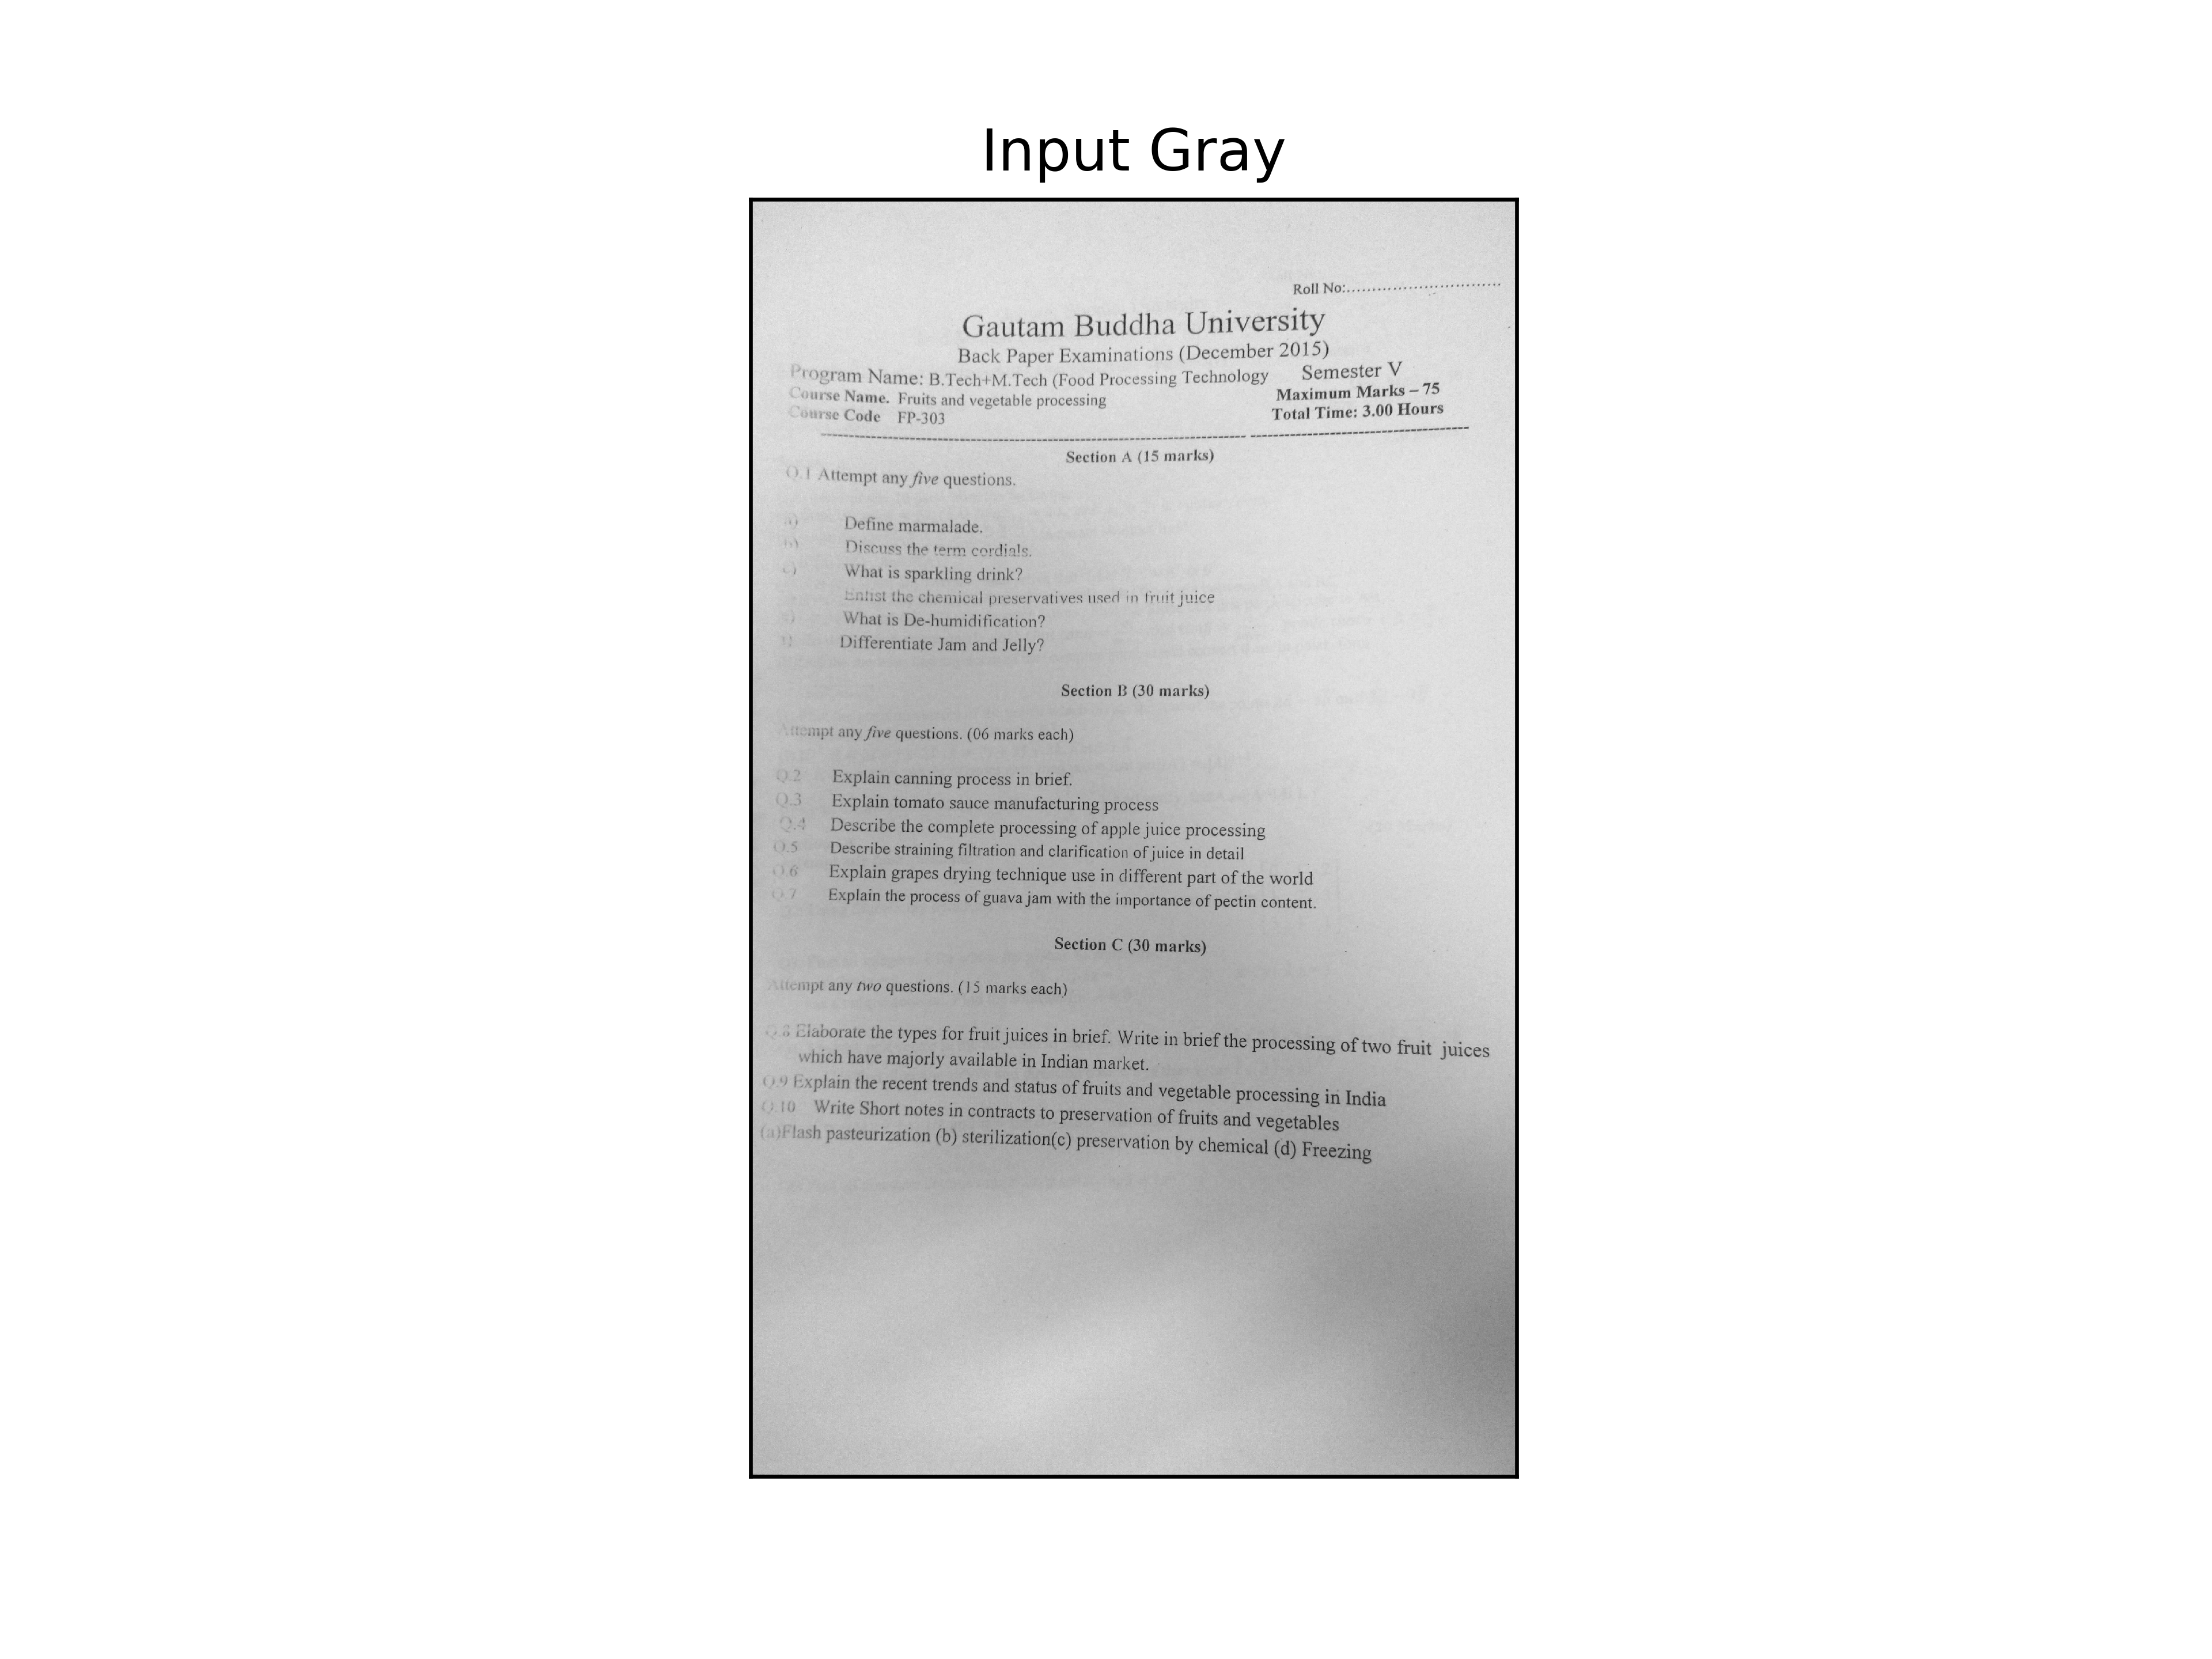
\includegraphics[width=0.32\textwidth]{img_5_gray.png}
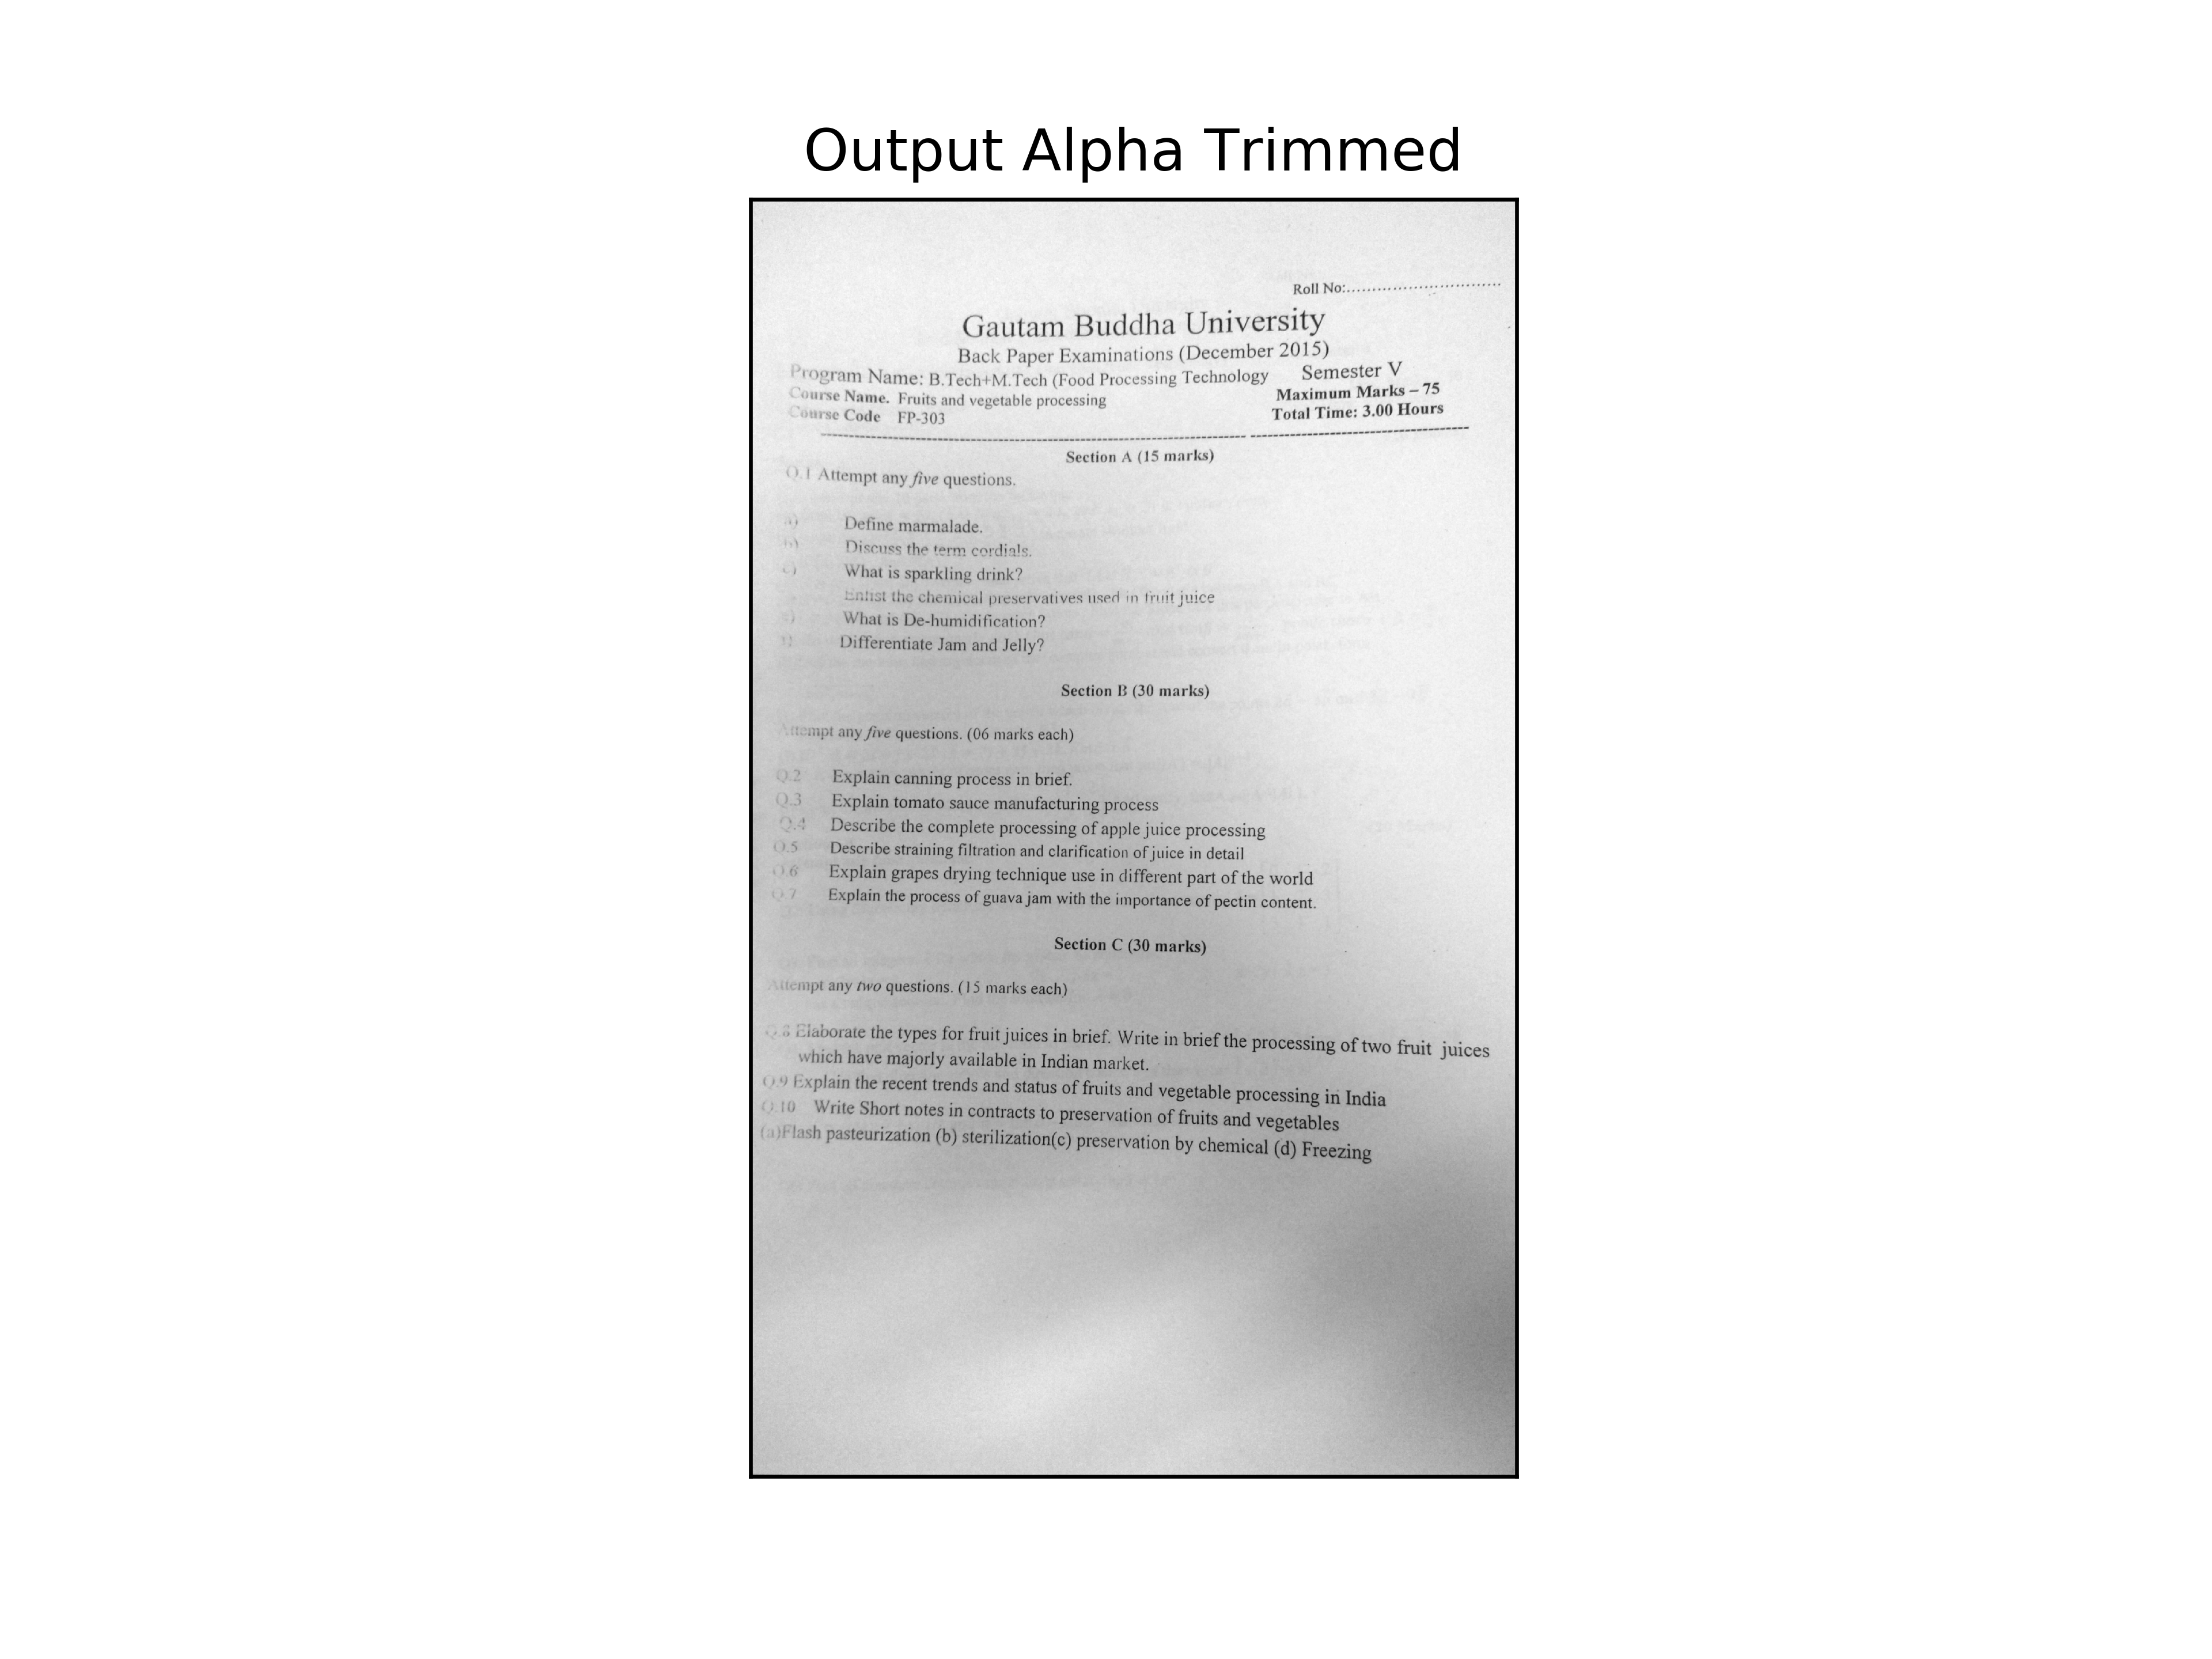
\includegraphics[width=0.32\textwidth]{img_5_output_alpha_trimmed.png}
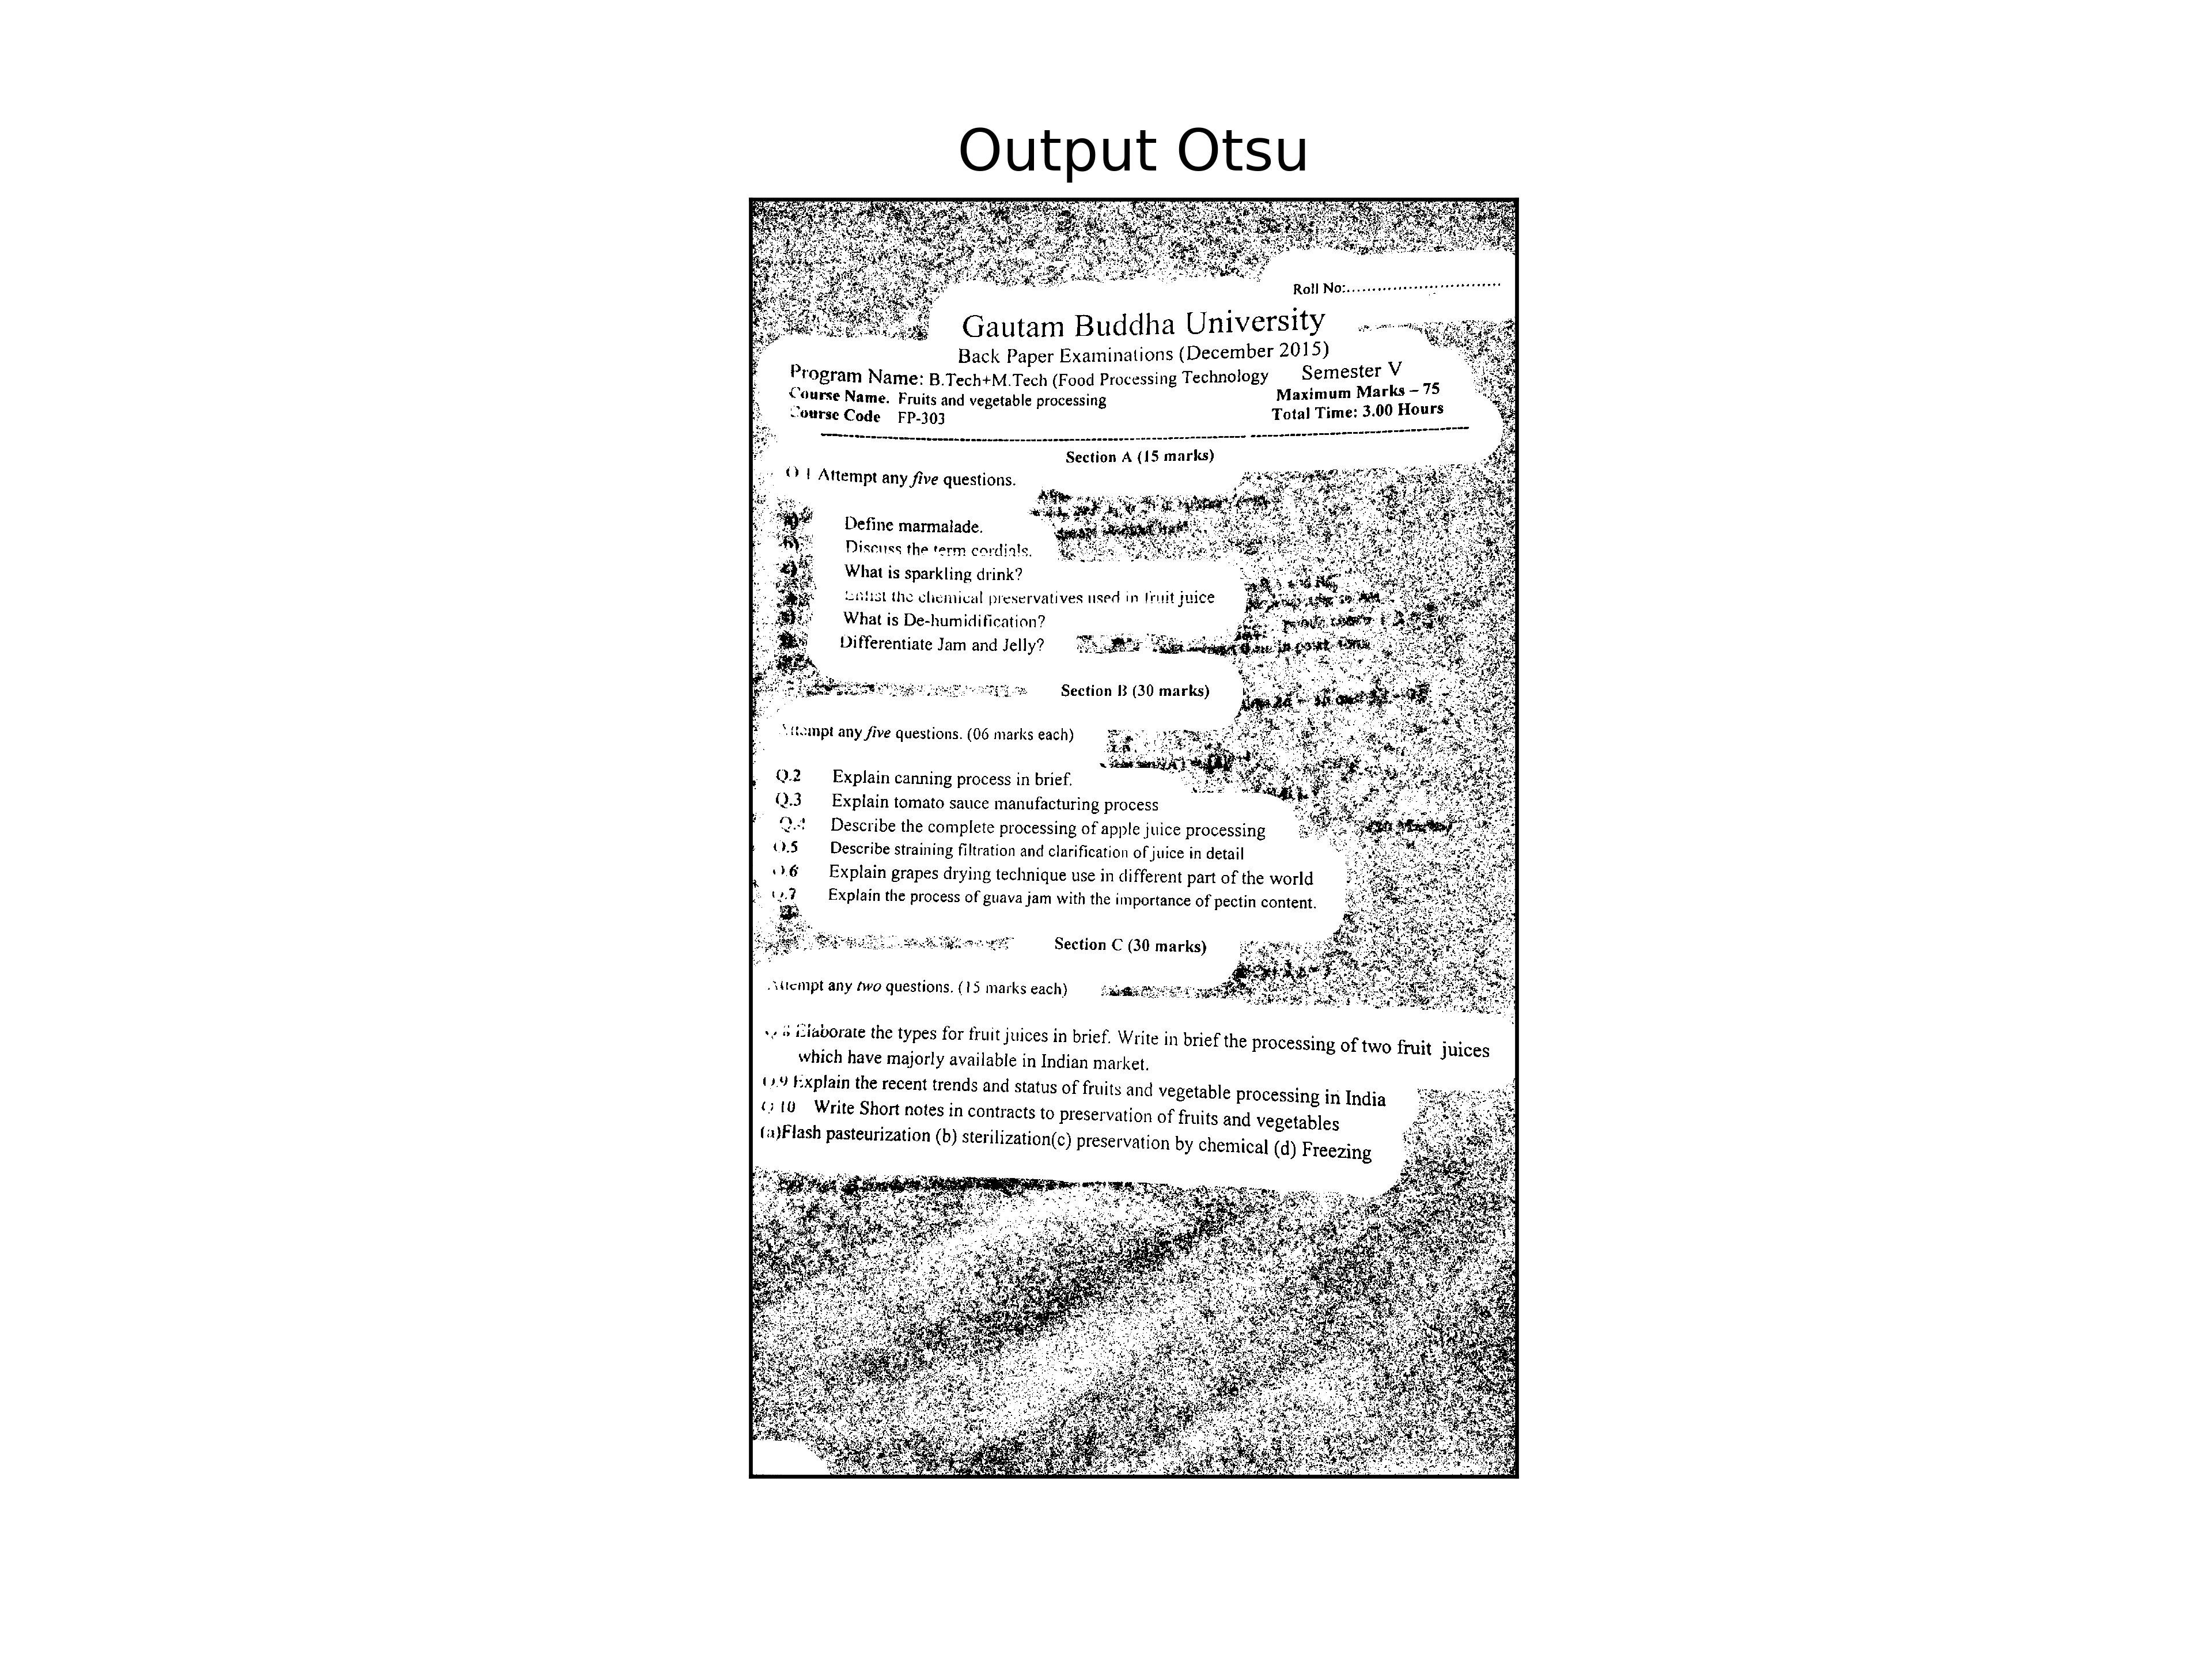
\includegraphics[width=0.32\textwidth]{img_5_output_otsu.png}
\end{center}

\begin{listing}
\begin{verbatim}
# Image 6, 7 
level = 2
# 1. k-means method
# thresh = mf.k_means_thresh(im_original_gray, level)
# t = np.pad(np.uint8(thresh), (1,), 'constant', constant_values=(0, 255))
# 2. Lloyd method
t = pp.lloyd_quantize(im_original_gray, level)
im_final = pp.gray_level_window_slice(im_original_gray, t, [0, 255])
\end{verbatim}
\centering
\caption{List 6: Setting For Image 6, 7}
\newline
\end{listing}

Image 6 and 7 can be processed by global threshold method. One way to find the
global threshold value is k-means algorithm. However, the time complexity of
k-means is much high. To decrease the time complexity, what I found is that
the Lloyd algorithm can also be used to find the threshold value by simply
setting the number of level in Lloyd algorithm to 2.

\begin{listing}
\begin{verbatim}
def lloyd_quantize(im_np, level=2):
    pix_count = collections.Counter(np.ravel(im_np))
    pix_count_total = len(np.ravel(im_np))
    t = np.zeros([level+1])
    r = np.zeros([level])
    # Initialize t with even gray-level distribution
    for k in range(level+1):
        t[k] = k / level * 255
    while True:
        check_done = True
        for k in range(level):
            r_num = 0
            r_den = 0
            for f in range(t[k].astype(np.uint8), t[k+1].astype(np.uint8)+1):
                pf = pix_count[f] / pix_count_total
                r_num += f * pf
                r_den += pf
            r[k] = r_num / r_den
        for k in range(1, level):
            temp = round((r[k] + r[k-1]) / 2)
            if temp != t[k]:
                t[k] = temp
                check_done = False
        if check_done is True:
            break
    return t.astype(np.uint8)
\end{verbatim}
\centering
\caption{List 7: Lloyd Algorithm For Global Threshold Implementation}
\newline
\end{listing}

\begin{listing}
\begin{verbatim}
def k_means_thresh(im_np, cluster=2):
    # centroid[current centroid value:sum:count]
    centroid = np.zeros([cluster, 3])
    for k in range(cluster):
        centroid[k, 0] = (k + .5) / cluster * 255
    im_height, im_width = im_np.shape
    while True:
        check_done = True
        for m in range(im_height):
            for n in range(im_width):
                min_dist = 99999
                cent_count = 0
                target_cent = 0
                for c in range(cluster):
                    distance = abs(im_np[m,n] - centroid[c, 0])
                    if distance < min_dist:
                        min_dist = distance
                        target_cent = cent_count
                    cent_count += 1
                centroid[target_cent, 1] += im_np[m,n]
                centroid[target_cent, 2] += 1
        for c in range(cluster):
            new_cent = centroid[c, 1] / centroid[c, 2]
            if abs(centroid[c, 0] - new_cent) >= 1:
                centroid[c, 0] = new_cent
                centroid[c, 1] = 0
                centroid[c, 2] = 0
                check_done = False
        if check_done:
            break
    thresh = np.zeros([cluster - 1])
    for c in range(1, cluster):
        thresh[c - 1] = (centroid[c - 1, 0] + centroid[c, 0]) / 2
    return thresh
\end{verbatim}
\centering
\caption{List 8: K-means Algorithm For Global Threshold Implementation}
\newline
\end{listing}

\begin{center}
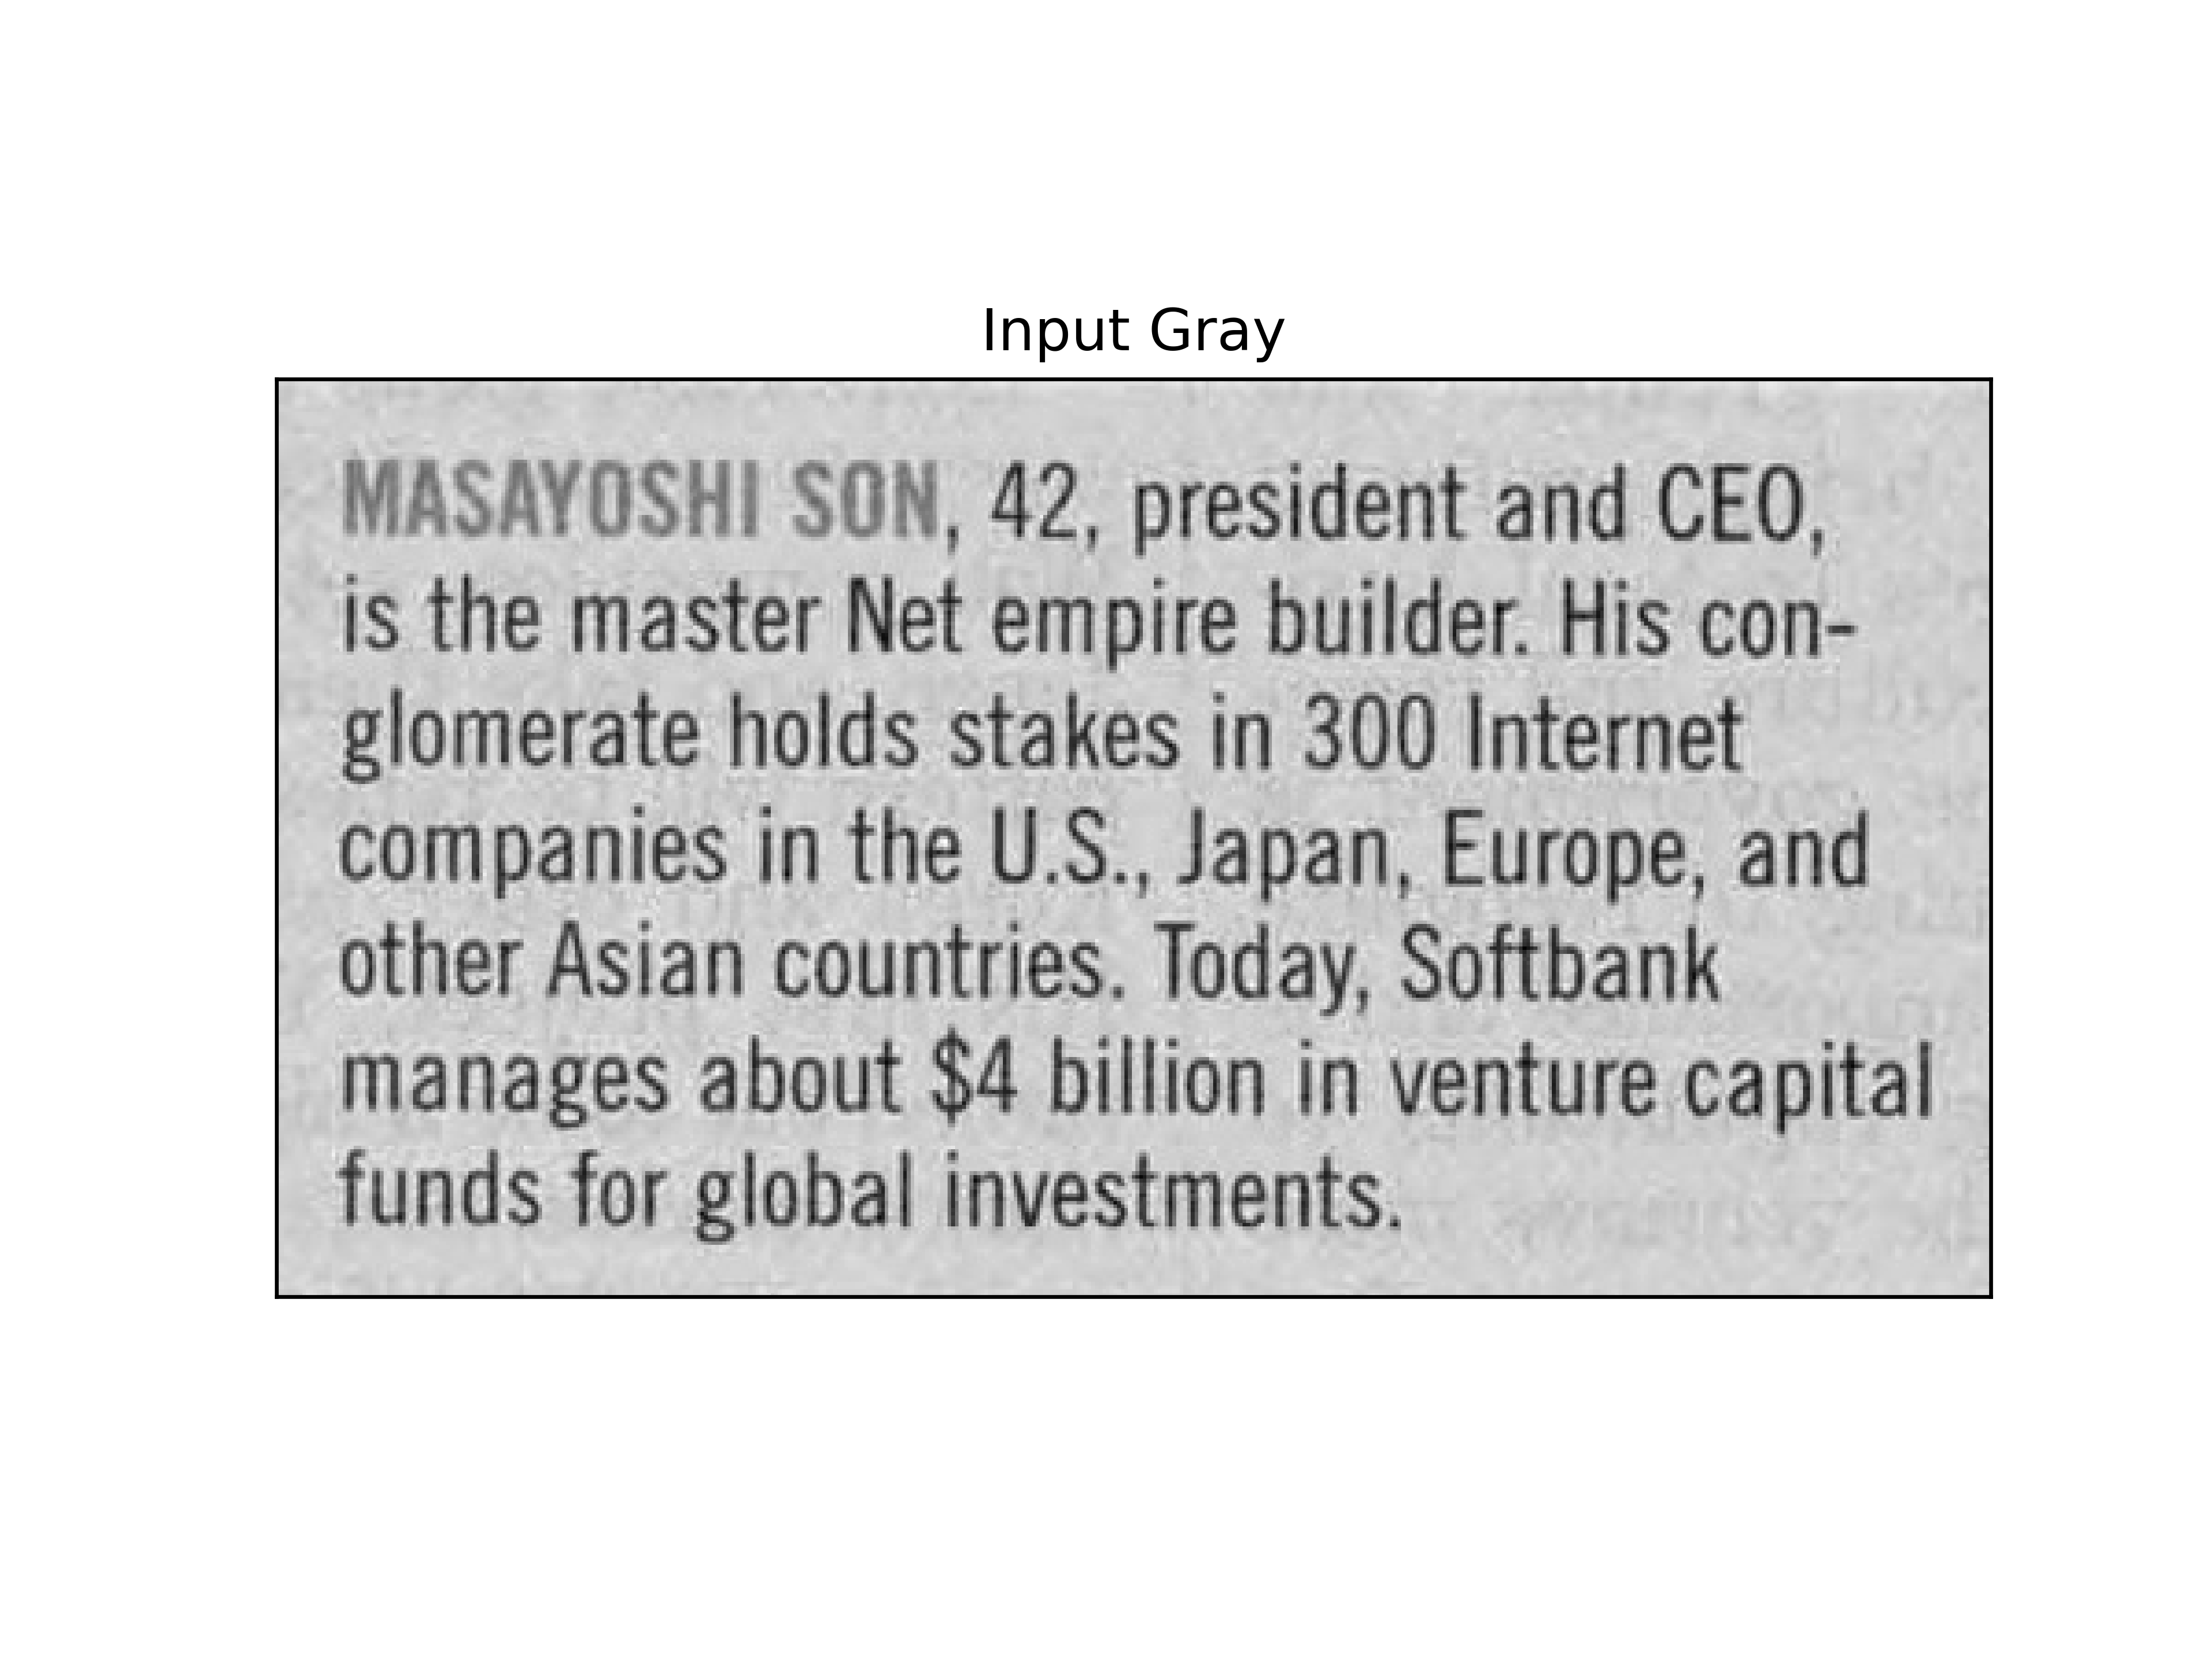
\includegraphics[width=0.49\textwidth]{img_6_gray.png}
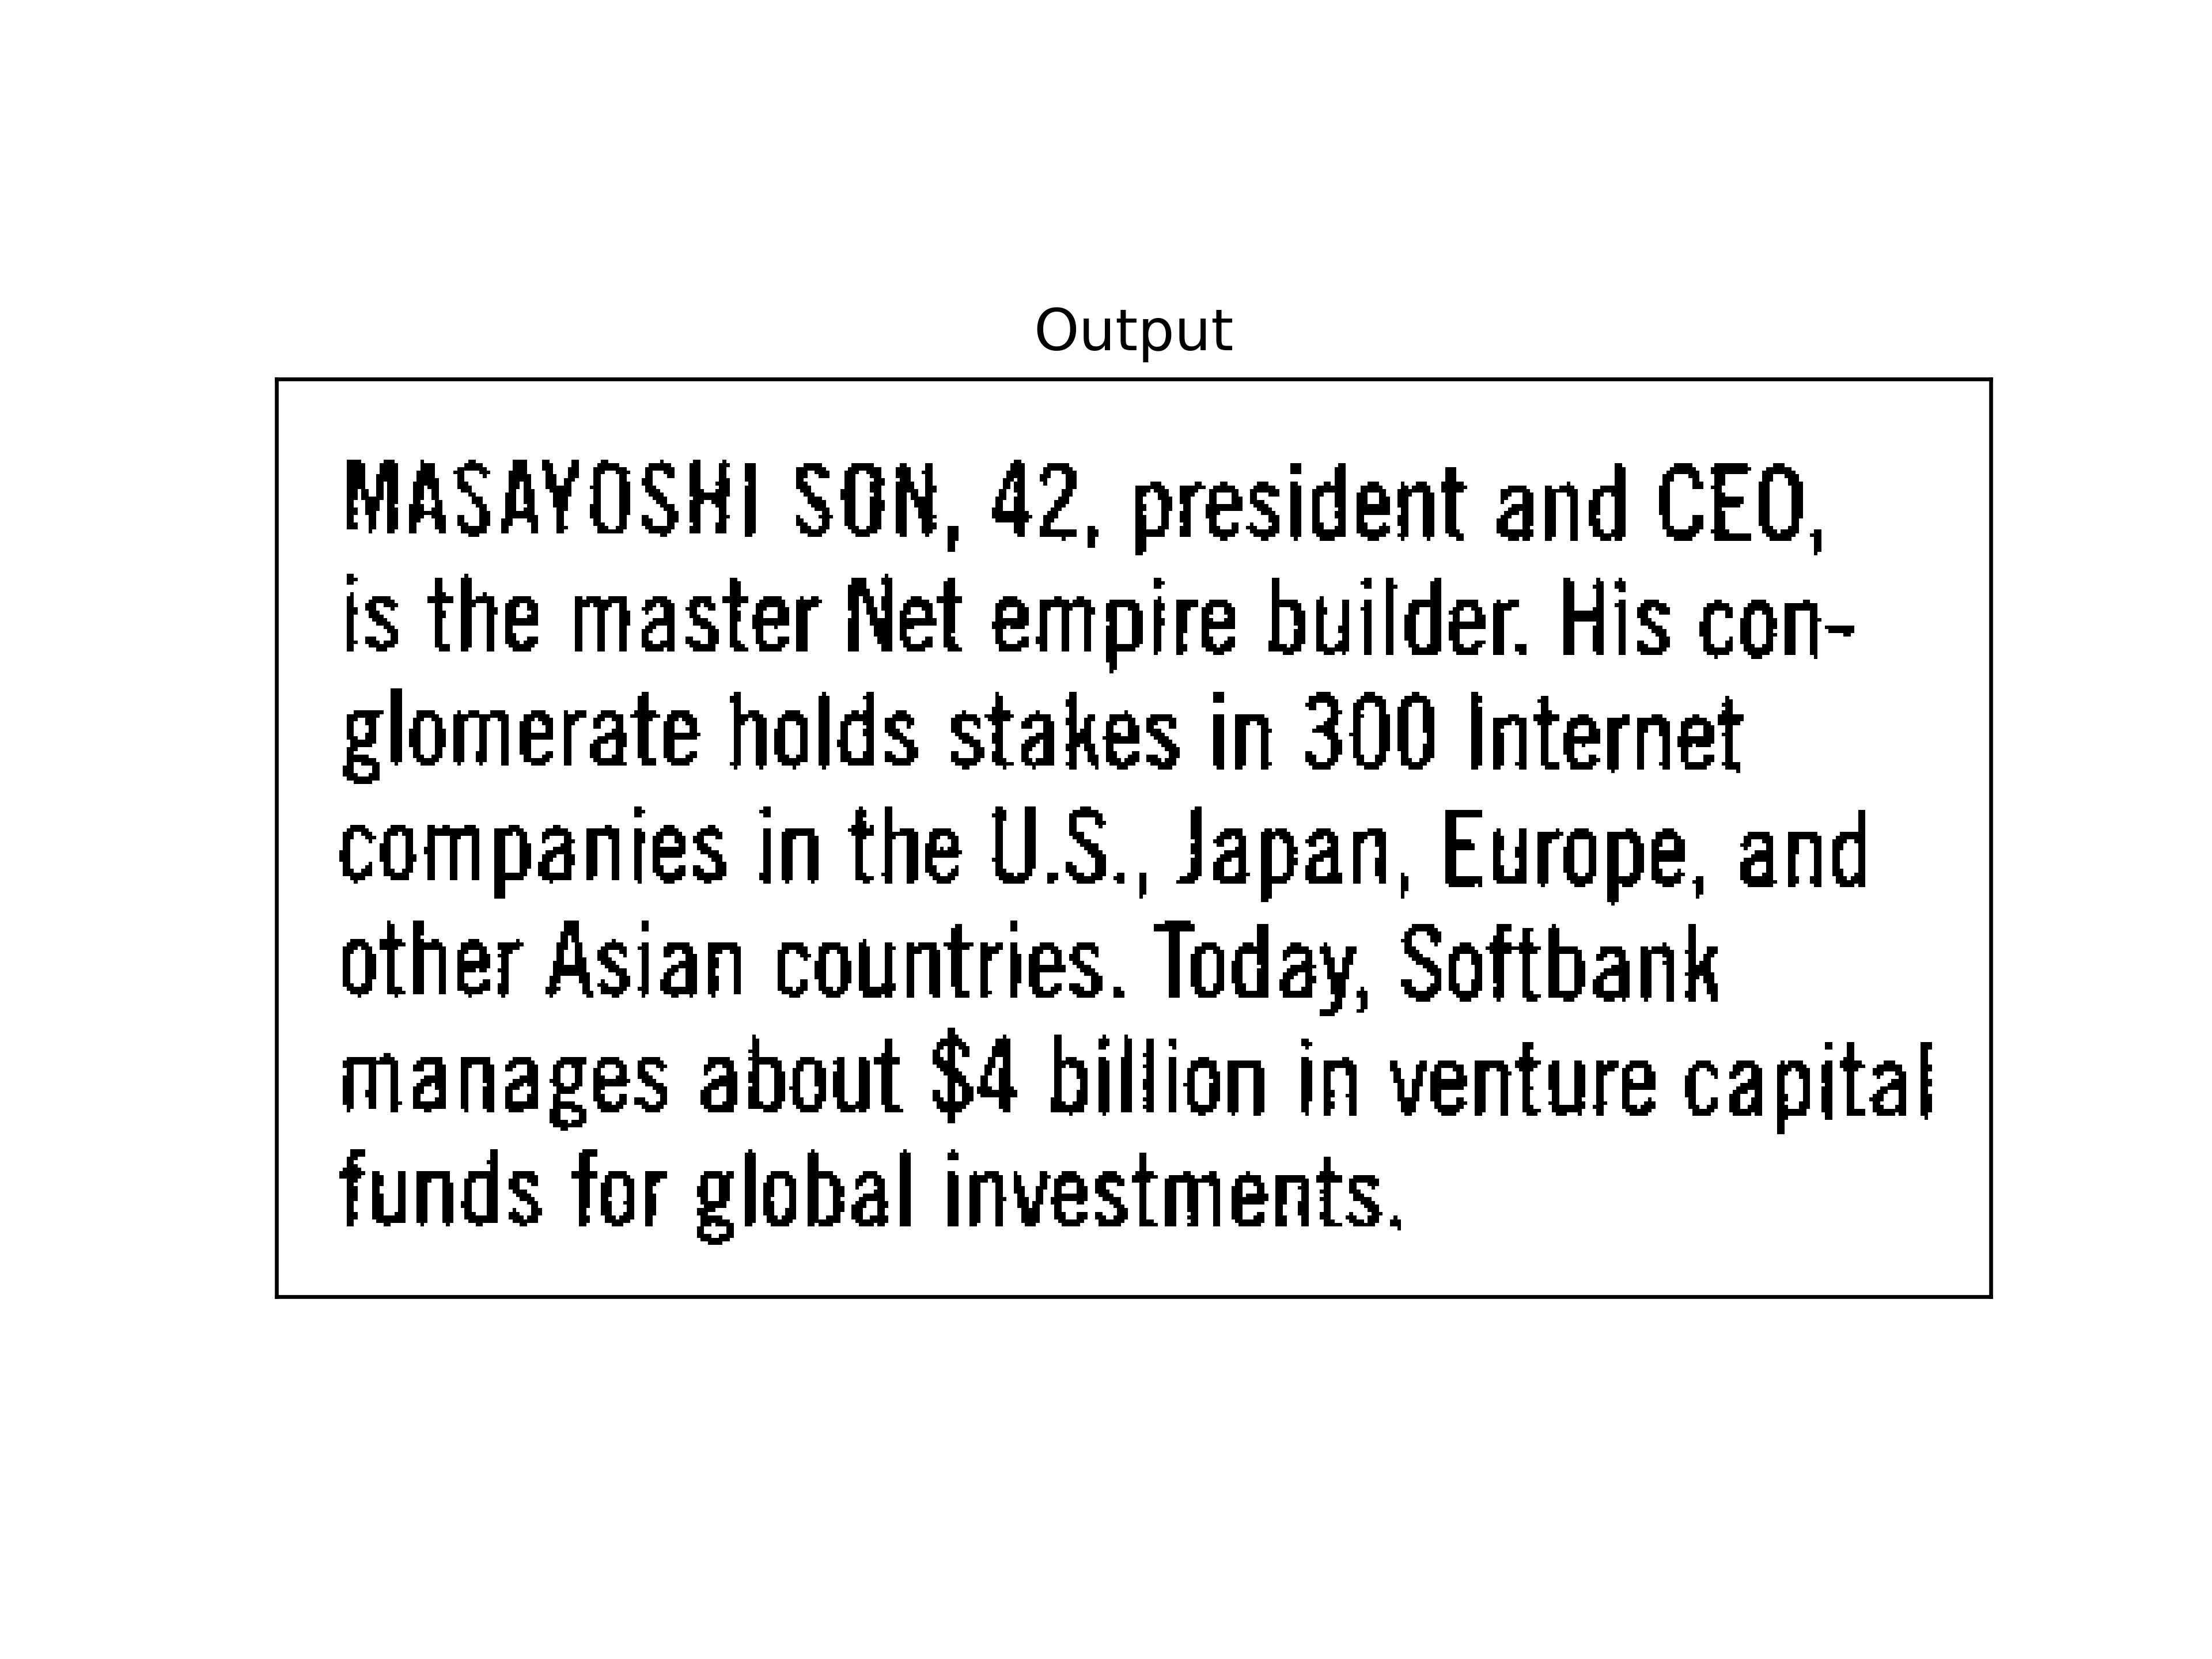
\includegraphics[width=0.49\textwidth]{img_6_output.png}
\end{center}

\begin{center}
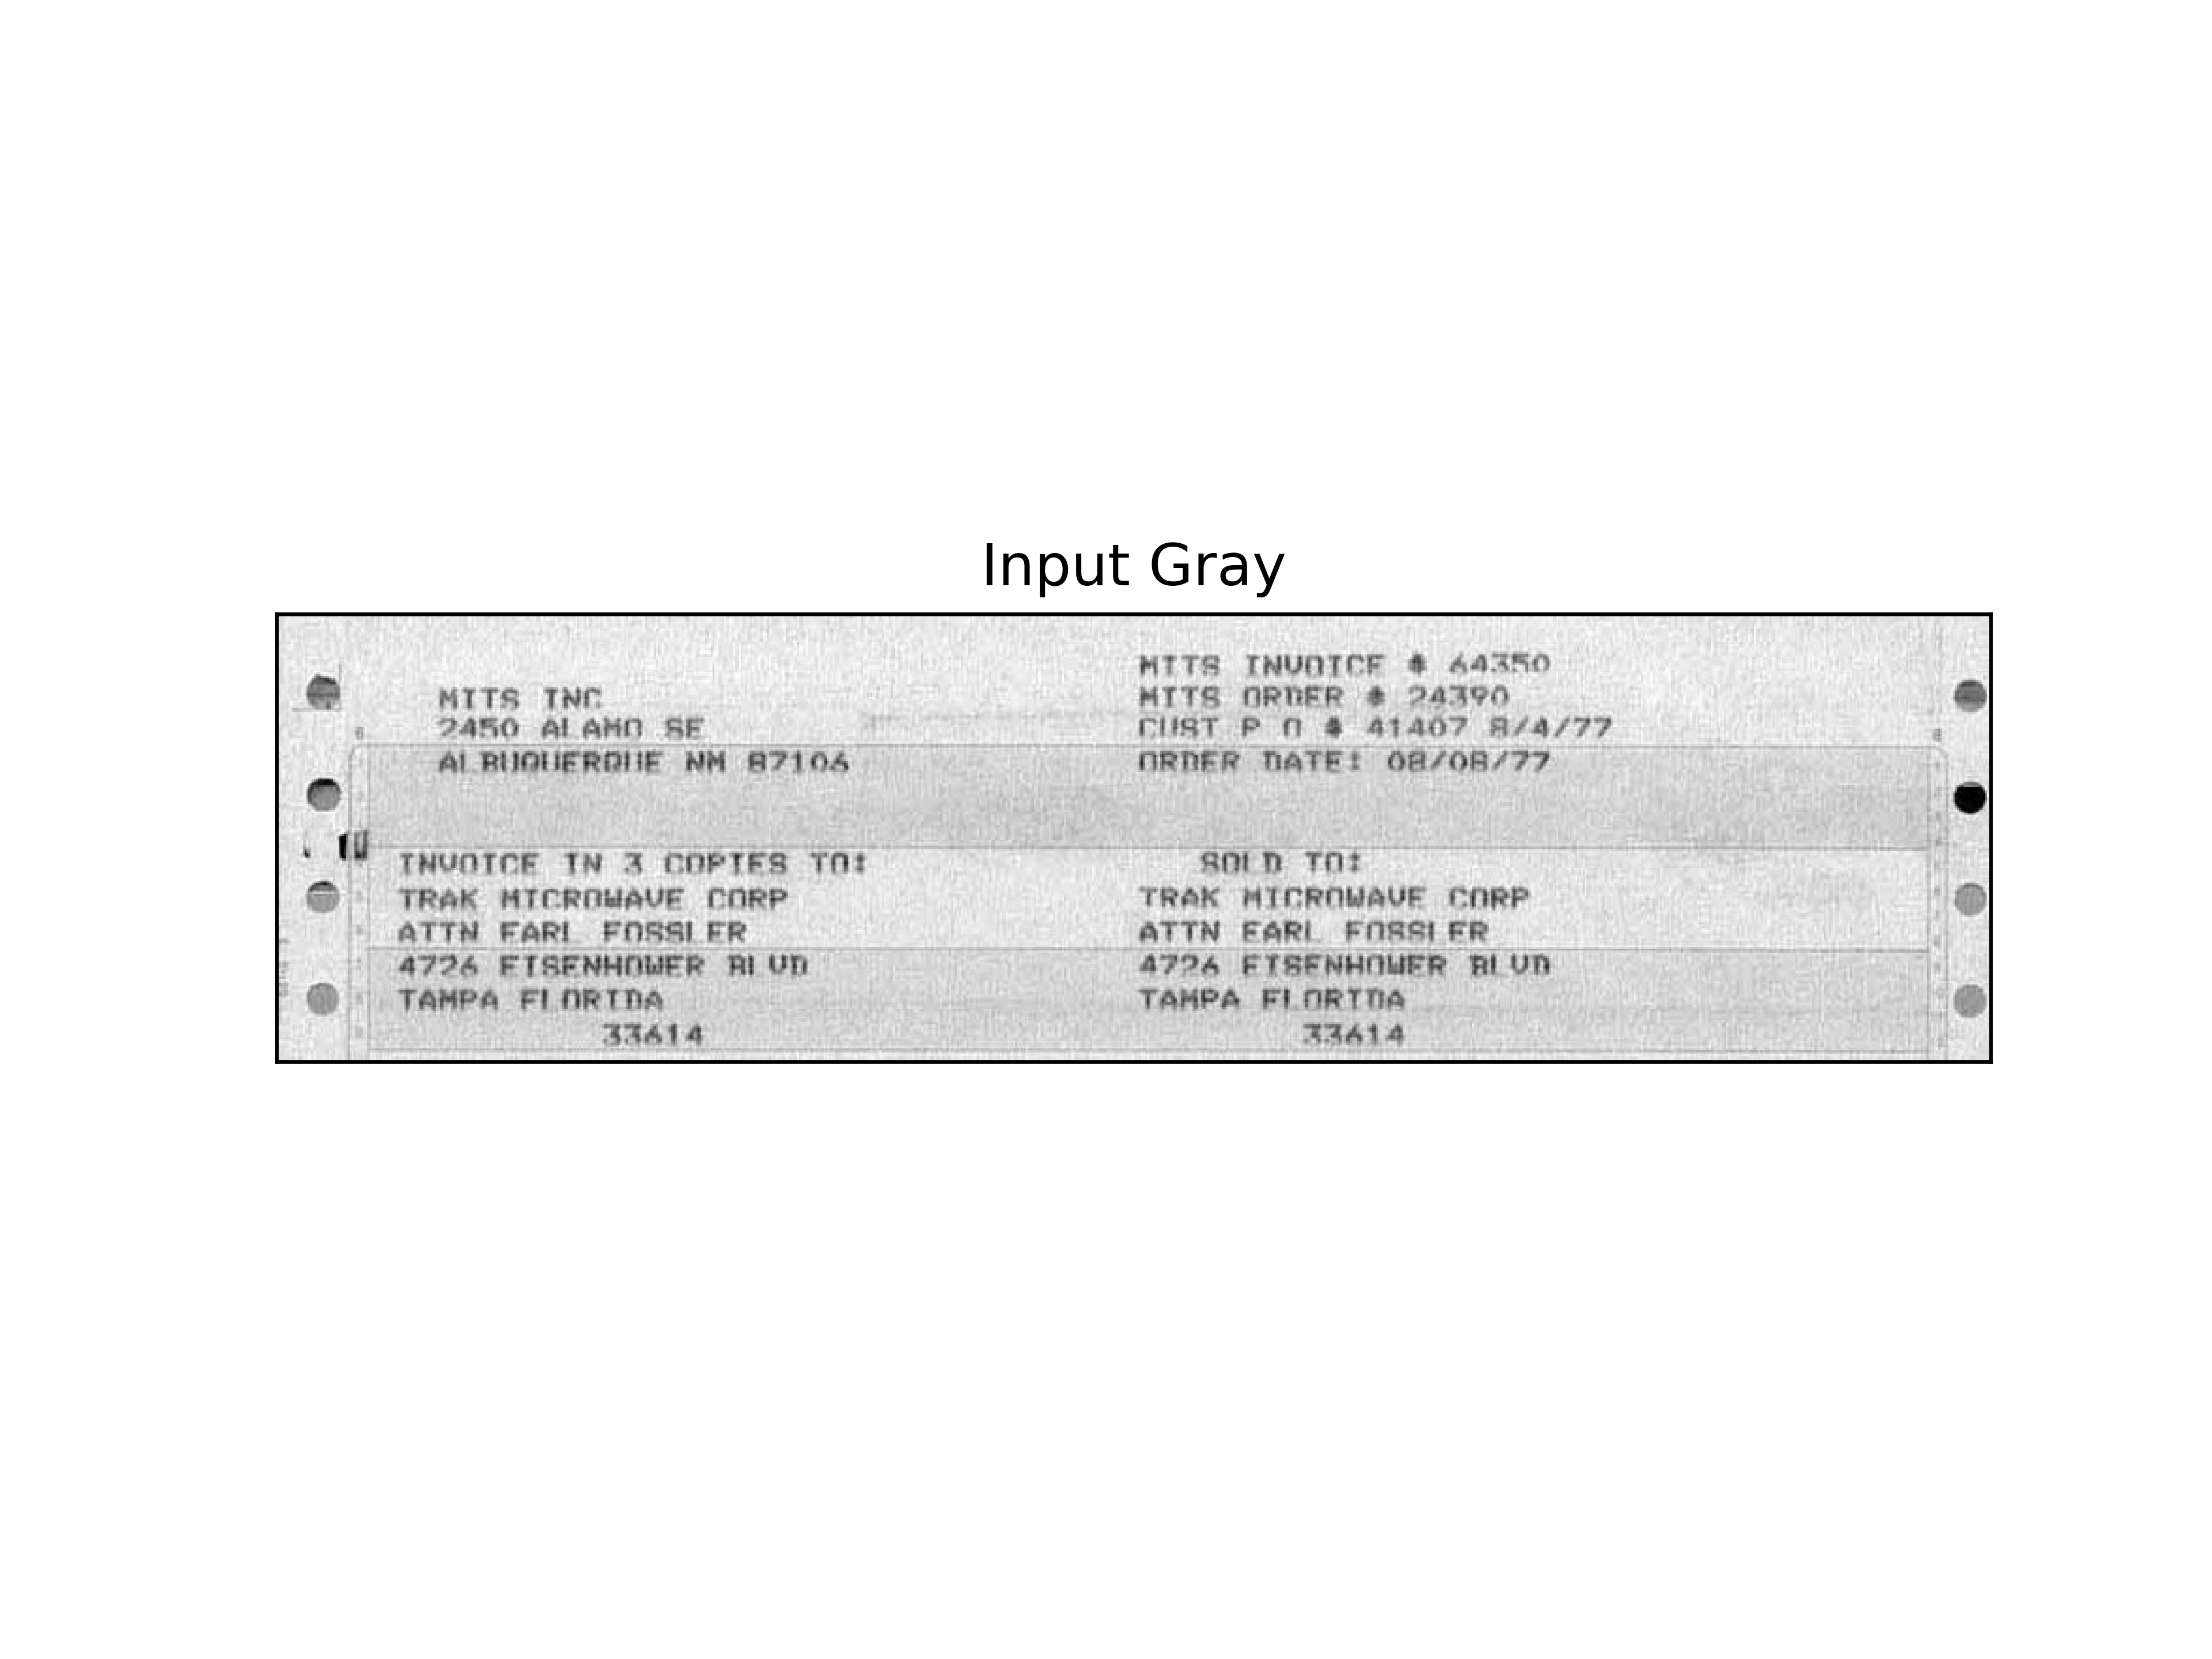
\includegraphics[width=0.49\textwidth]{img_7_gray.png}
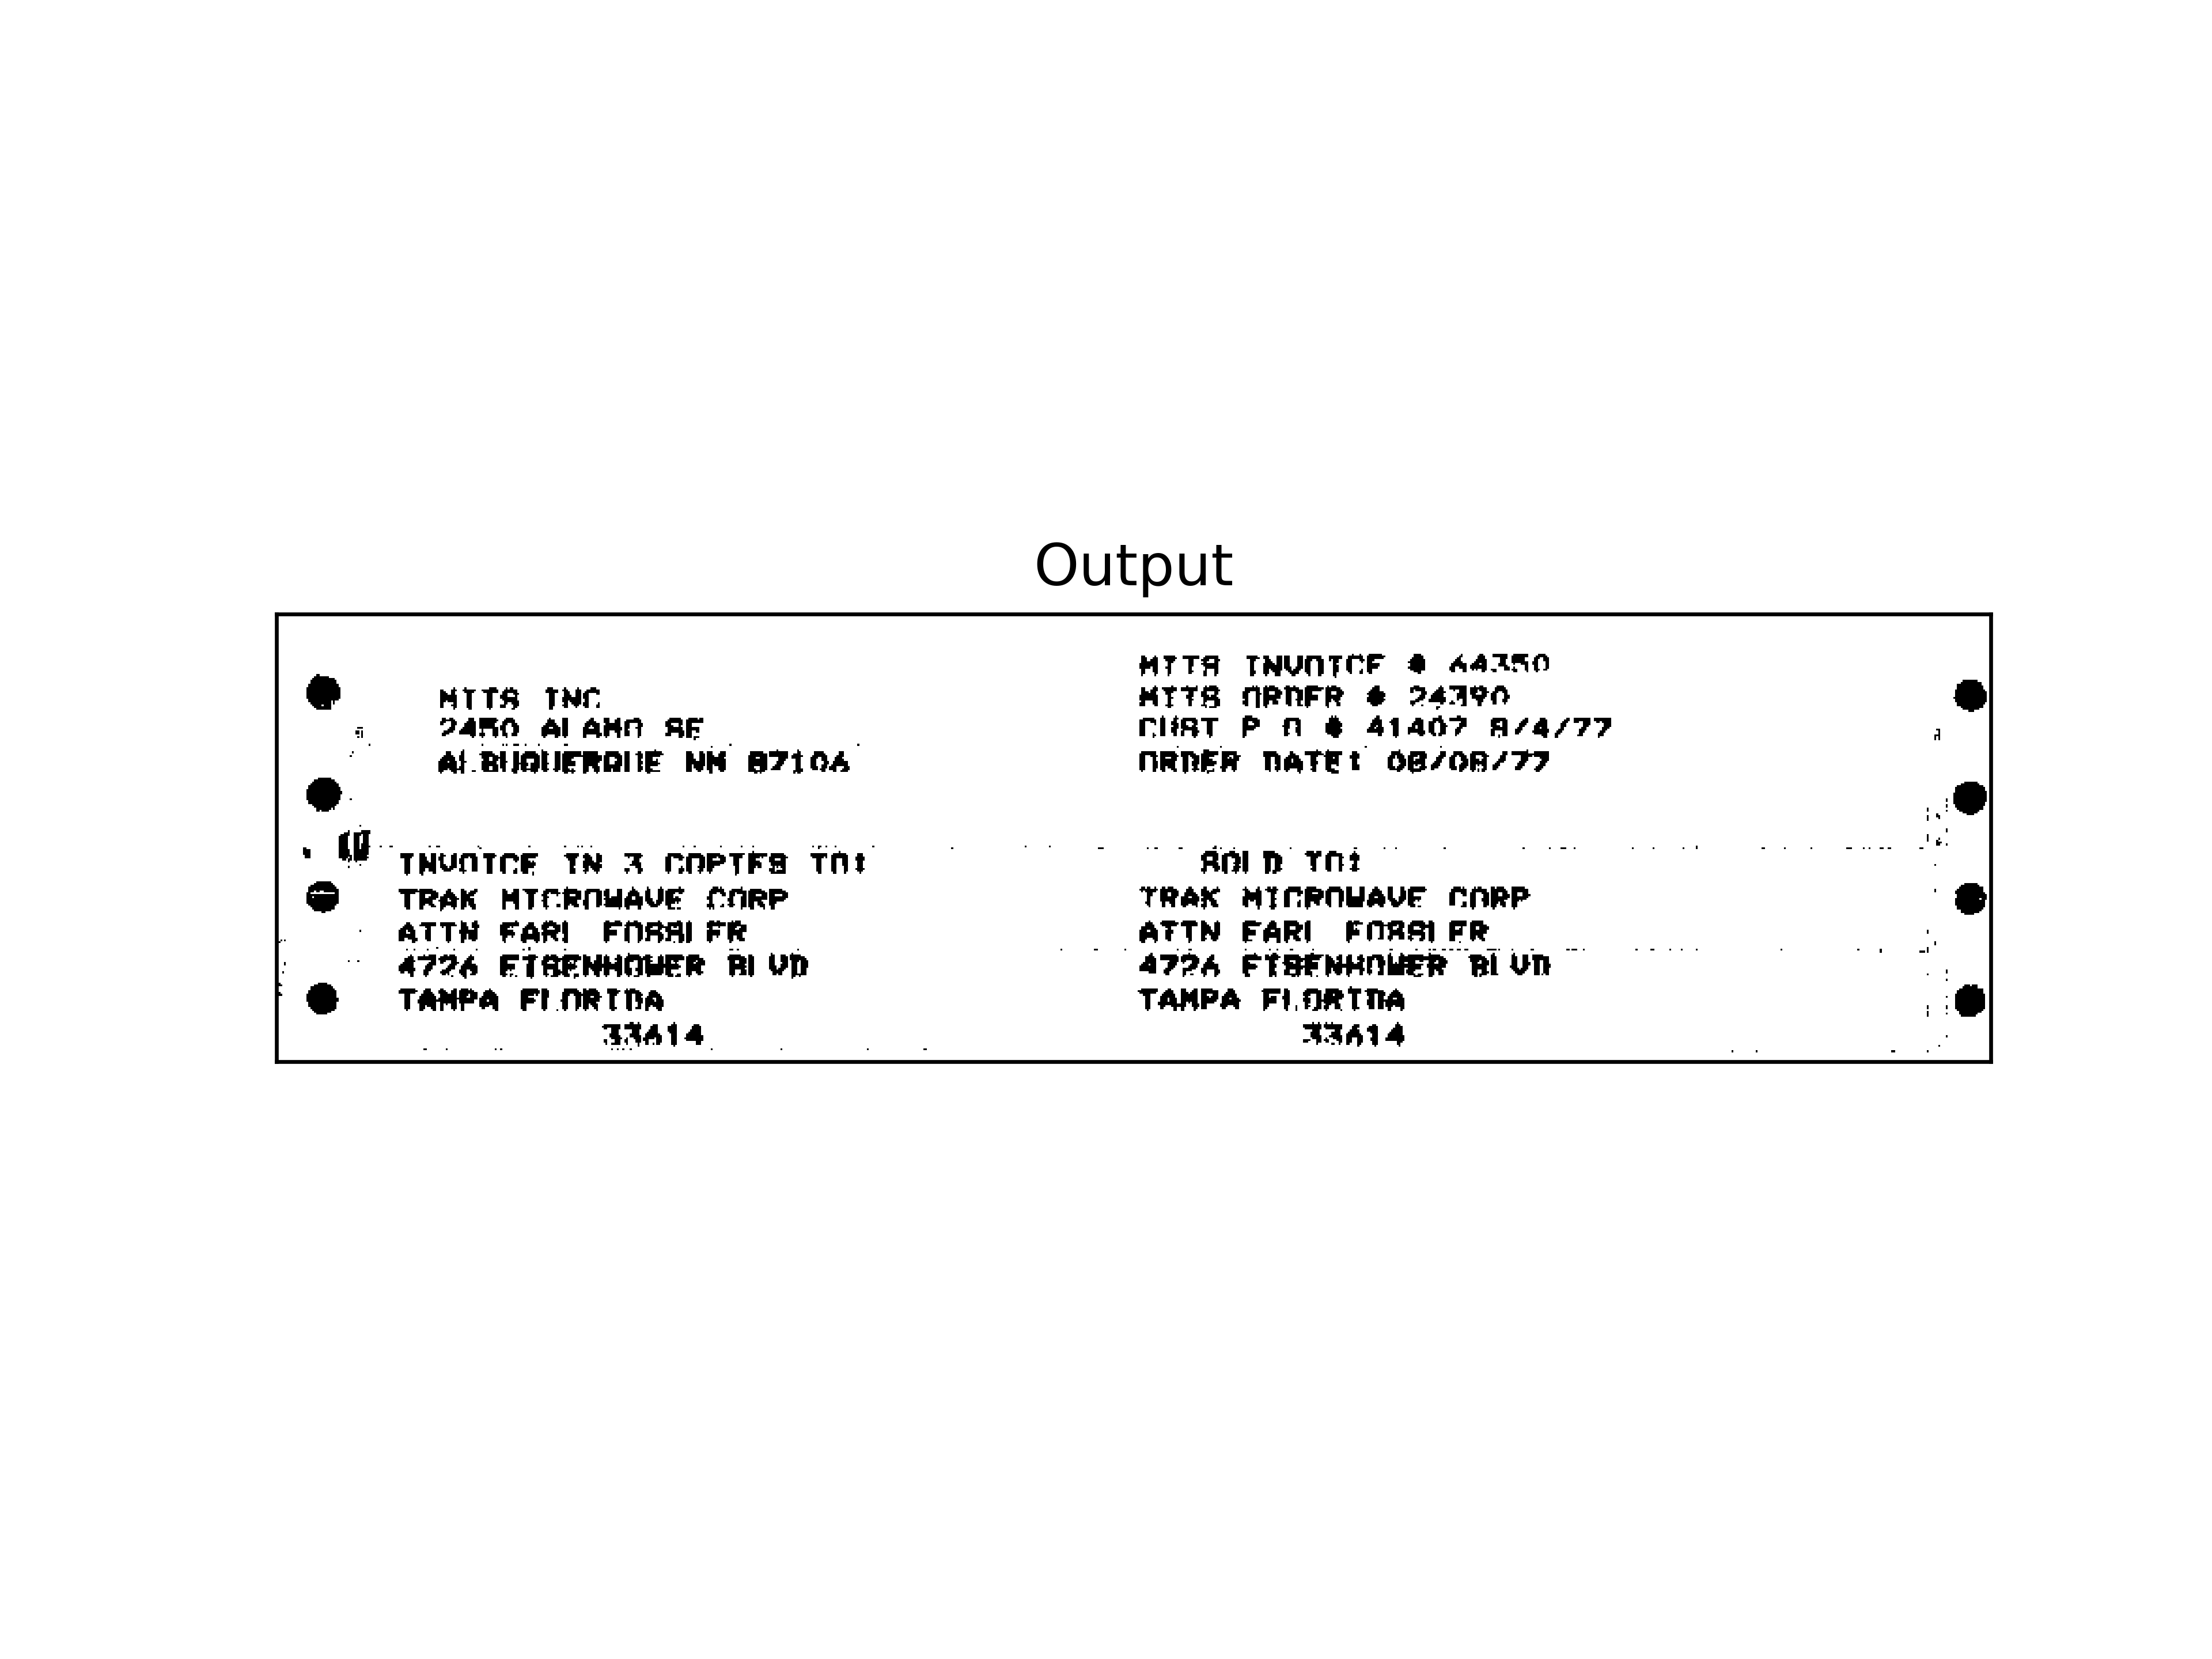
\includegraphics[width=0.49\textwidth]{img_7_output.png}
\end{center}

To process image 8, which has blurred text and un-even contrast distribution,
it is difficult to apply global threshold directly. However, the result is not
satisfied even after performing contrast stretching, like what I do on
image 9. To improve the image quality, firstly, it should be resized to 4
times larger than the original size. Then it can be applied the global
threshold method, which is implemented through Lloyd algorithm.

\begin{listing}
\begin{verbatim}
# Image 8 
im_step_1 = imresize(im_original_gray, (im_original_gray.shape[0] * 4, im_original_gray.shape[1] * 4))
level = 2
t = pp.lloyd_quantize(im_step_1, level)
im_final = pp.gray_level_window_slice(im_step_1, t, [0, 255])
\end{verbatim}
\centering
\caption{List 9: Setting For Image 8}
\newline
\end{listing}

\begin{center}
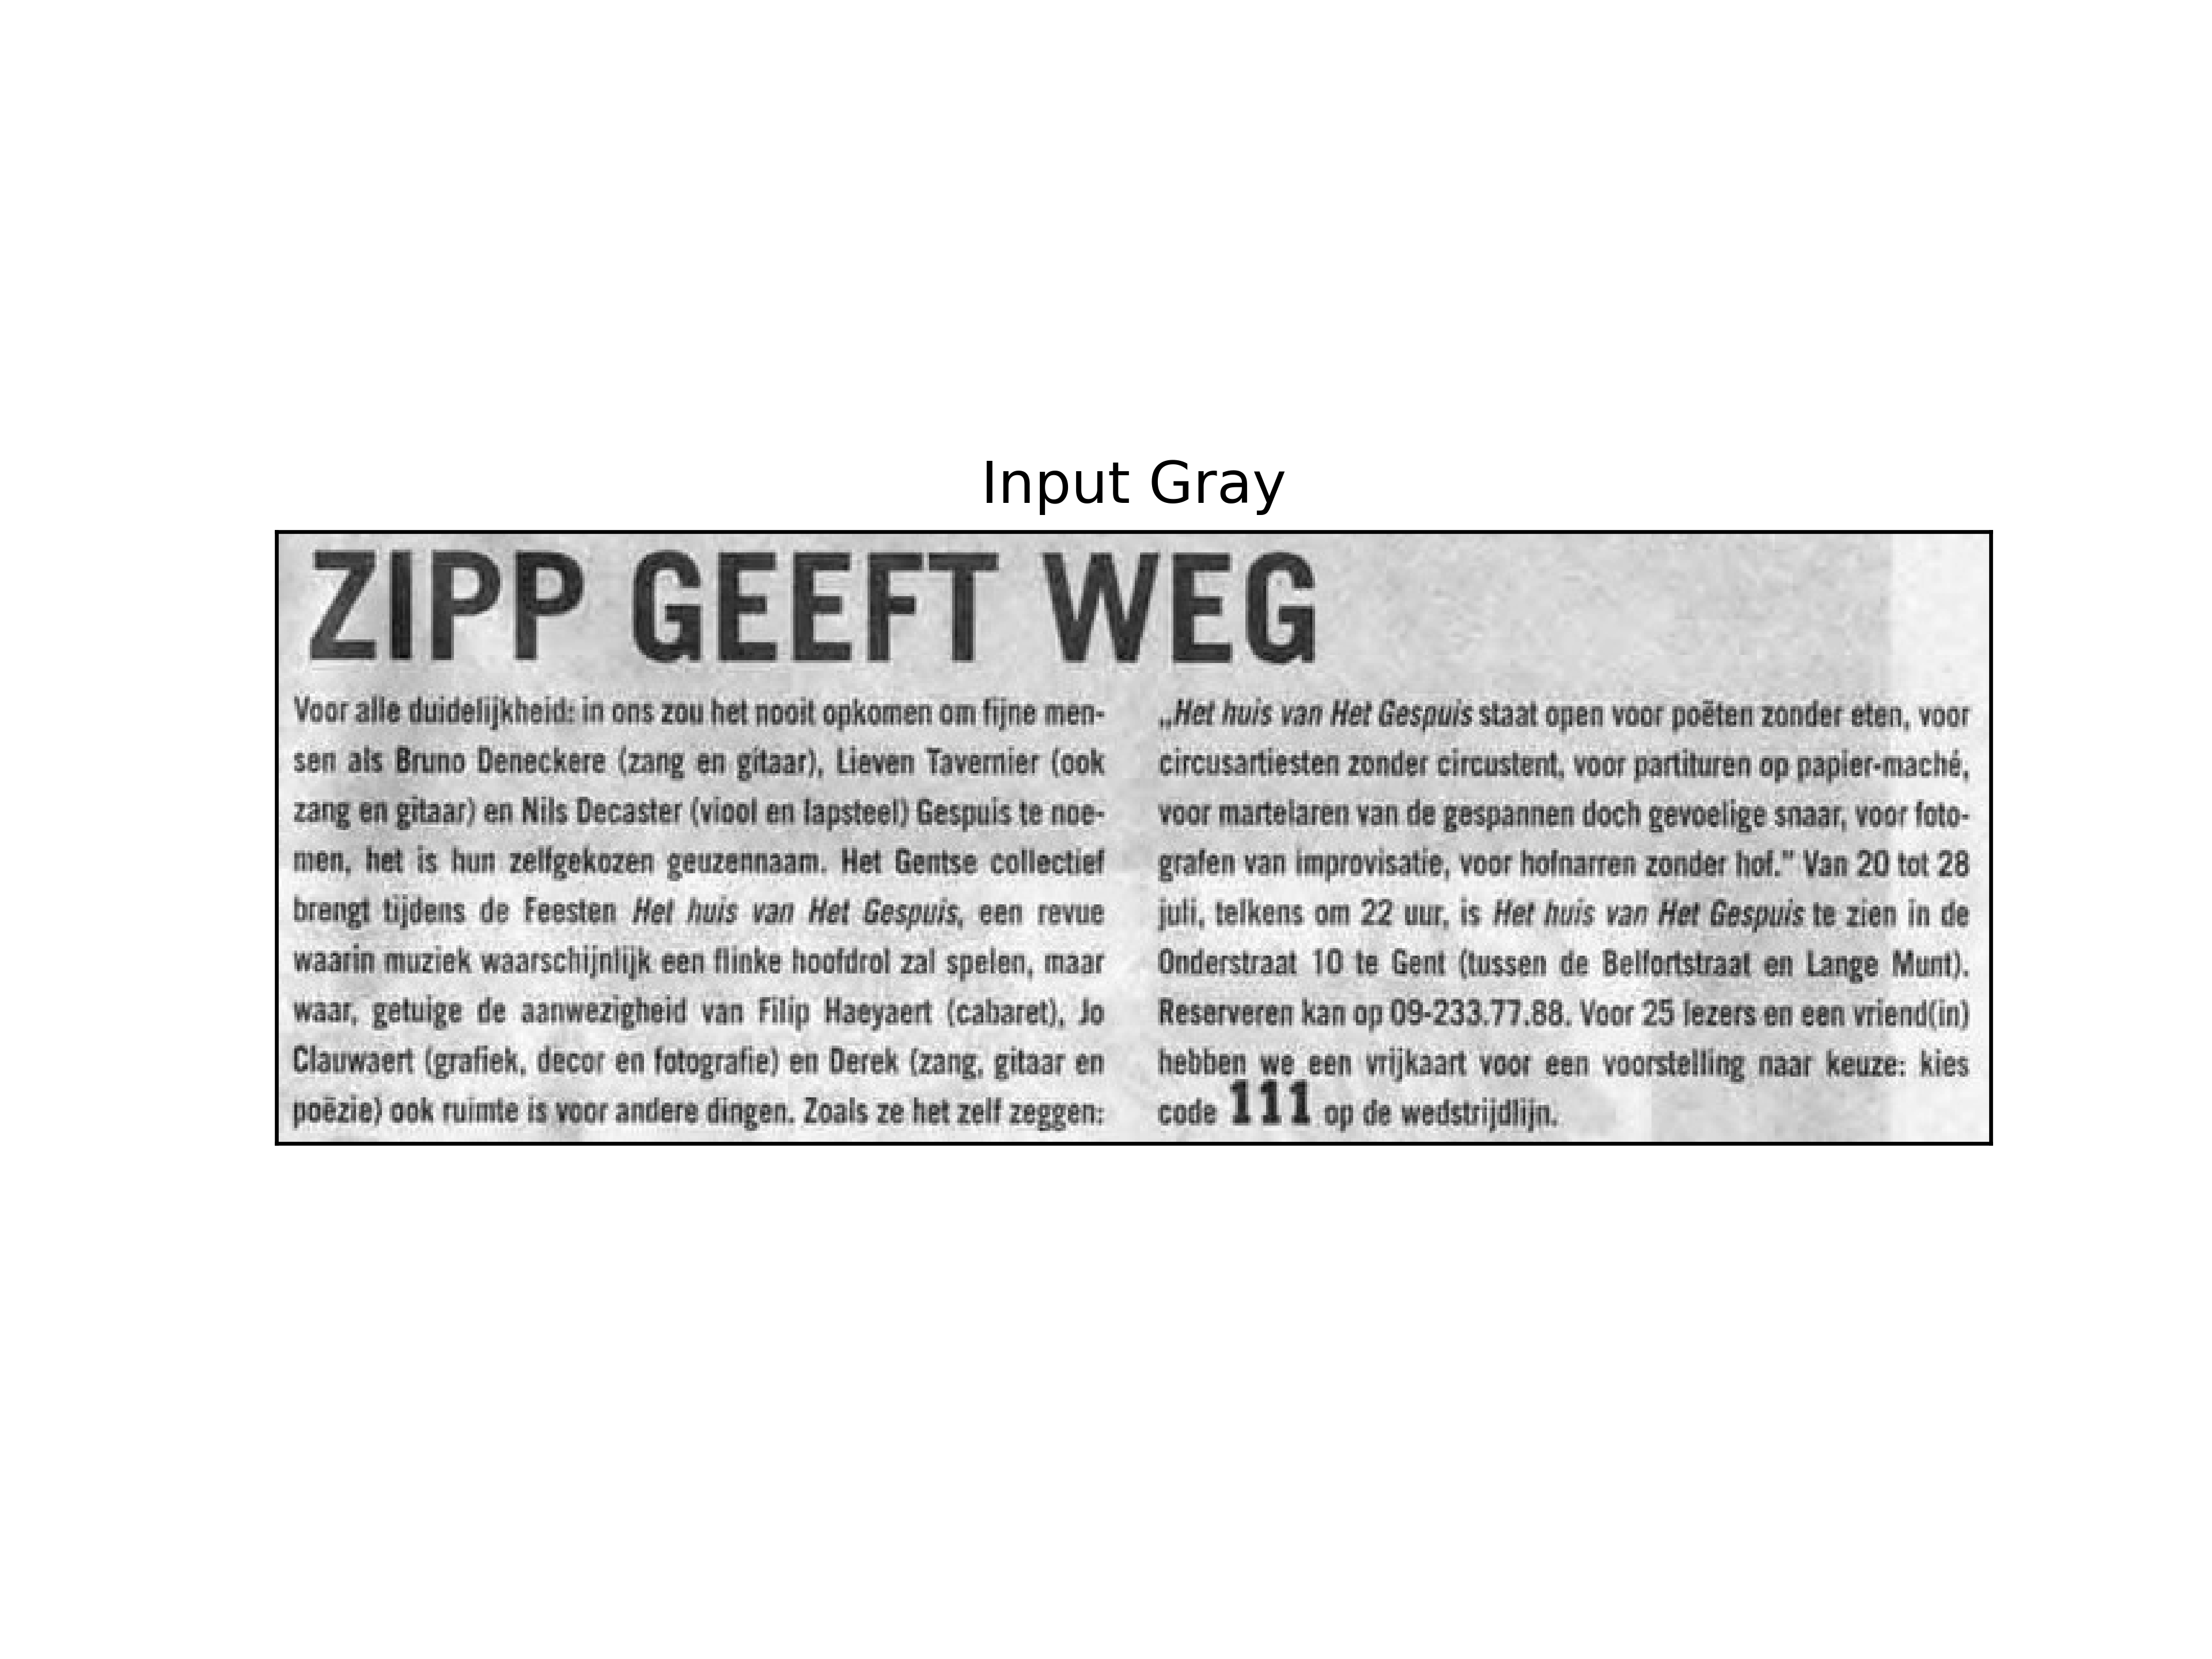
\includegraphics[width=0.32\textwidth]{img_8_gray.png}
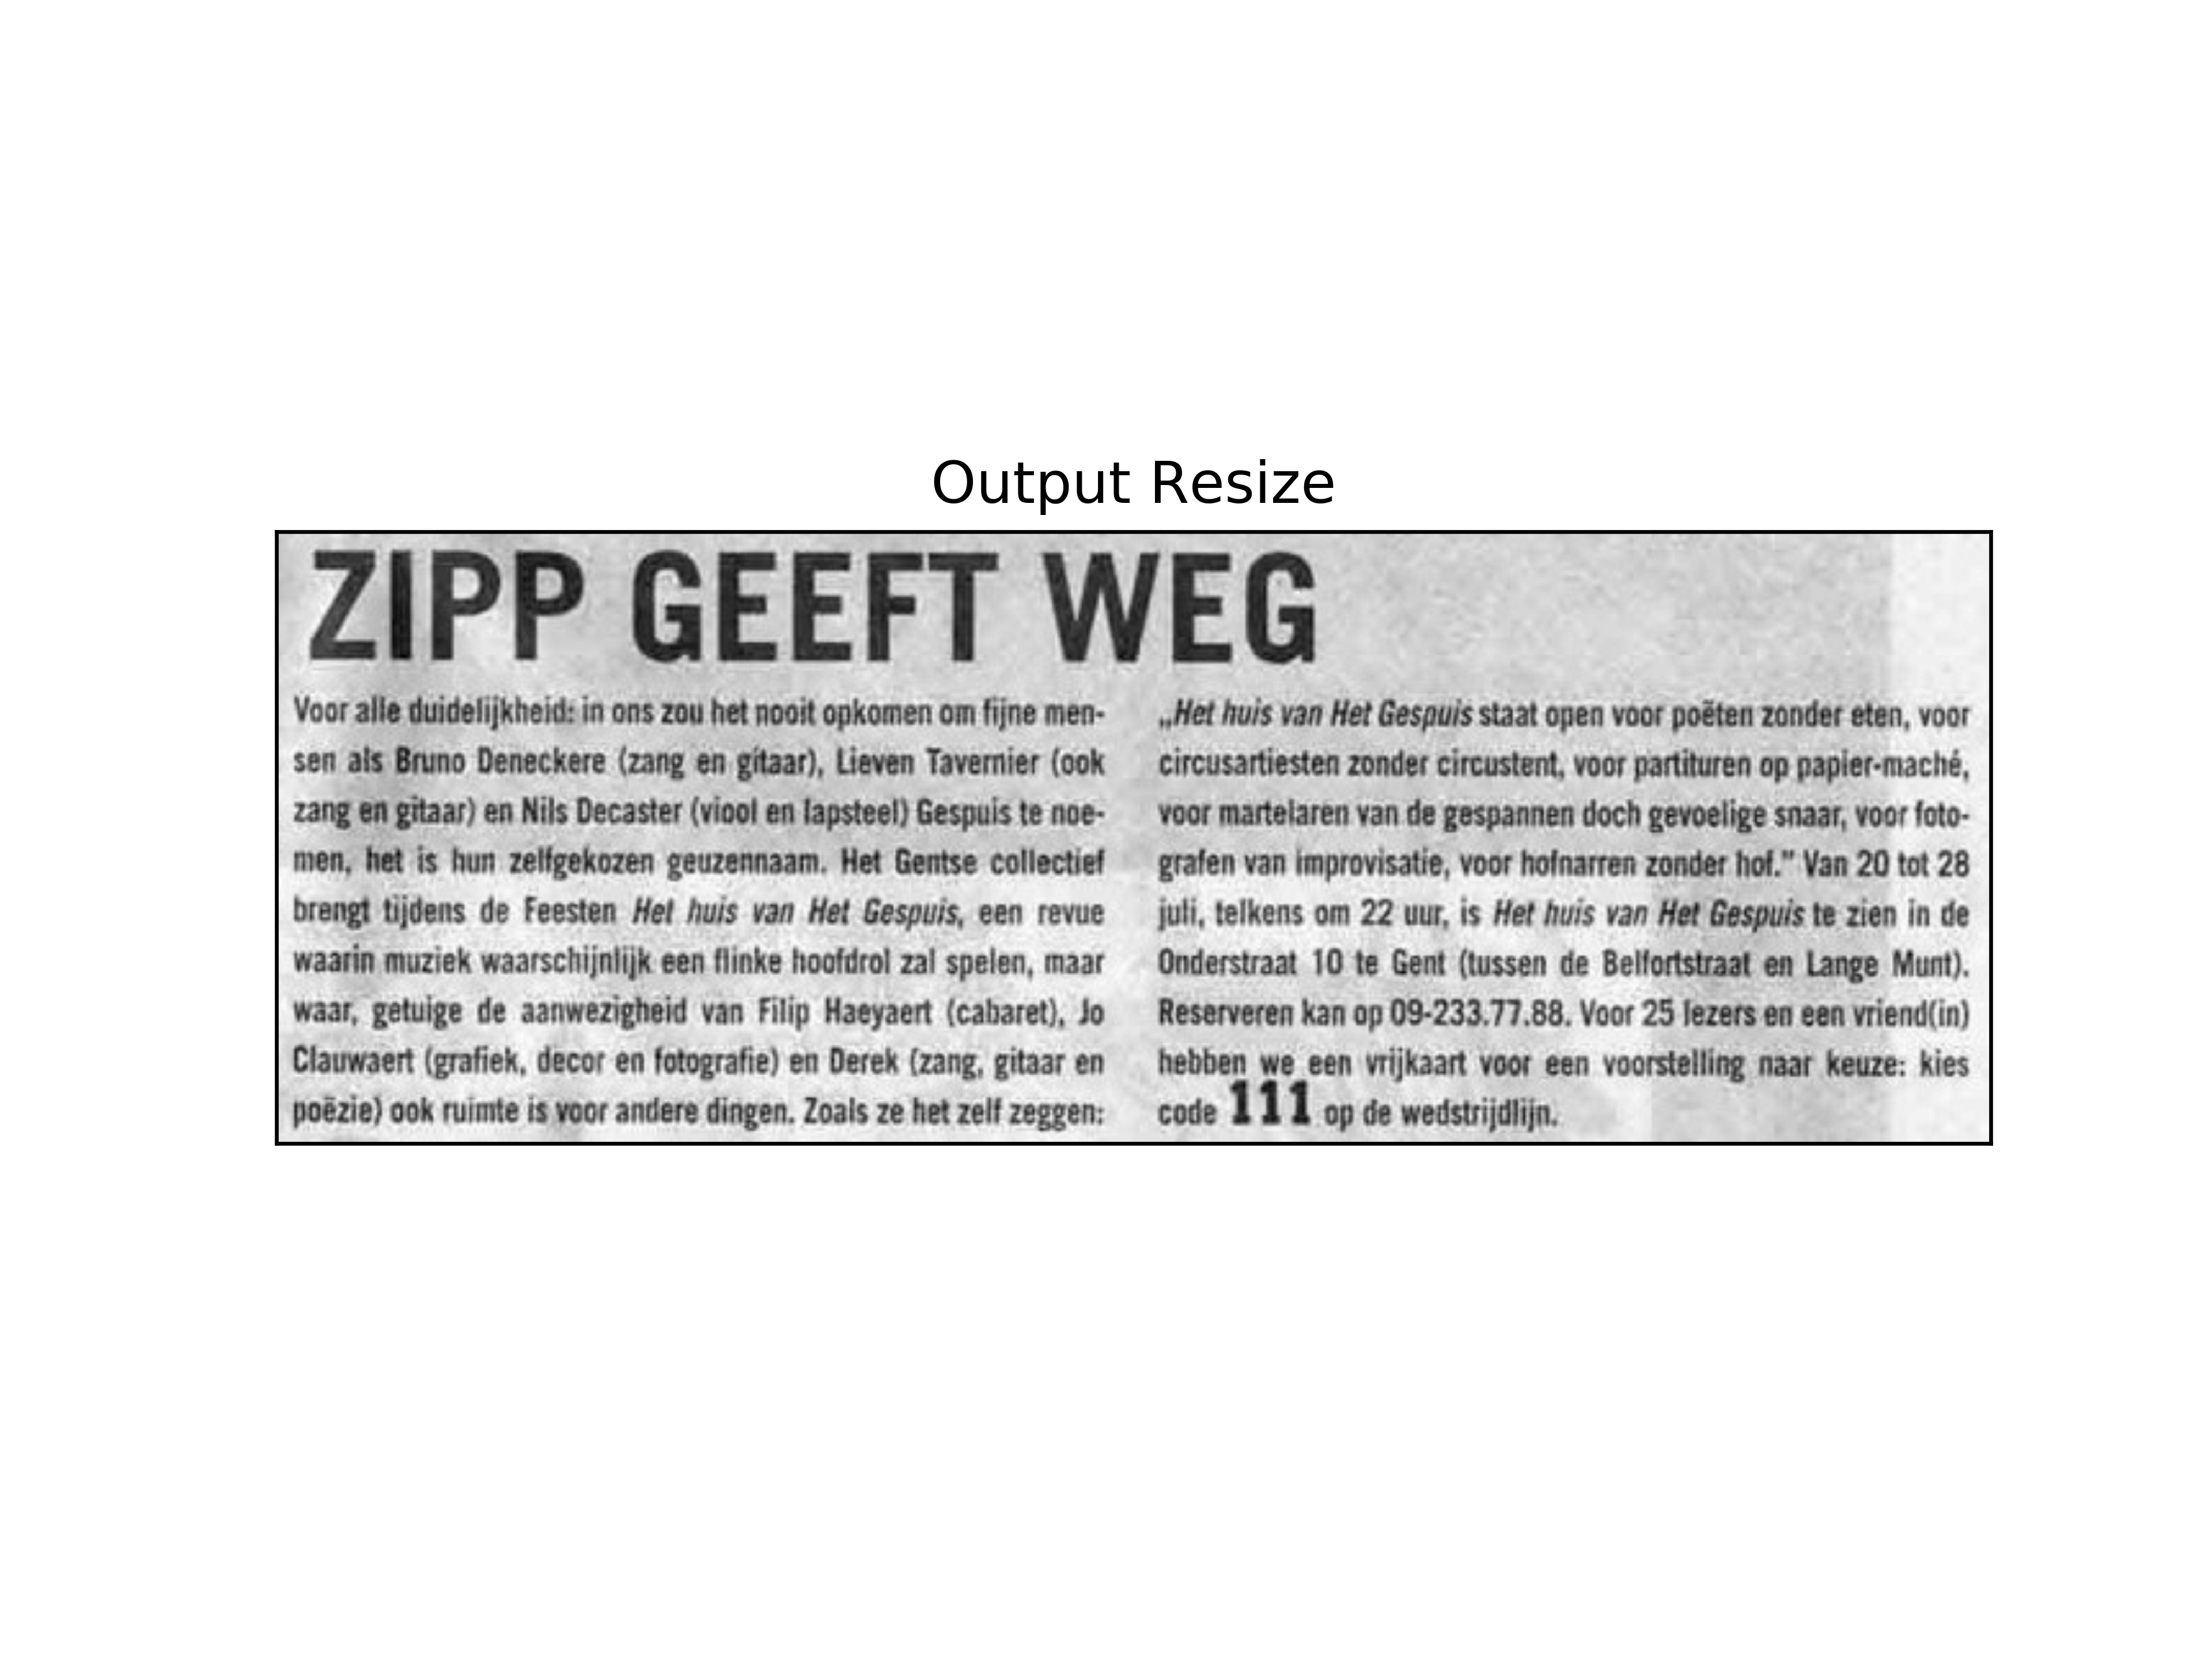
\includegraphics[width=0.32\textwidth]{img_8_output_resize.png}
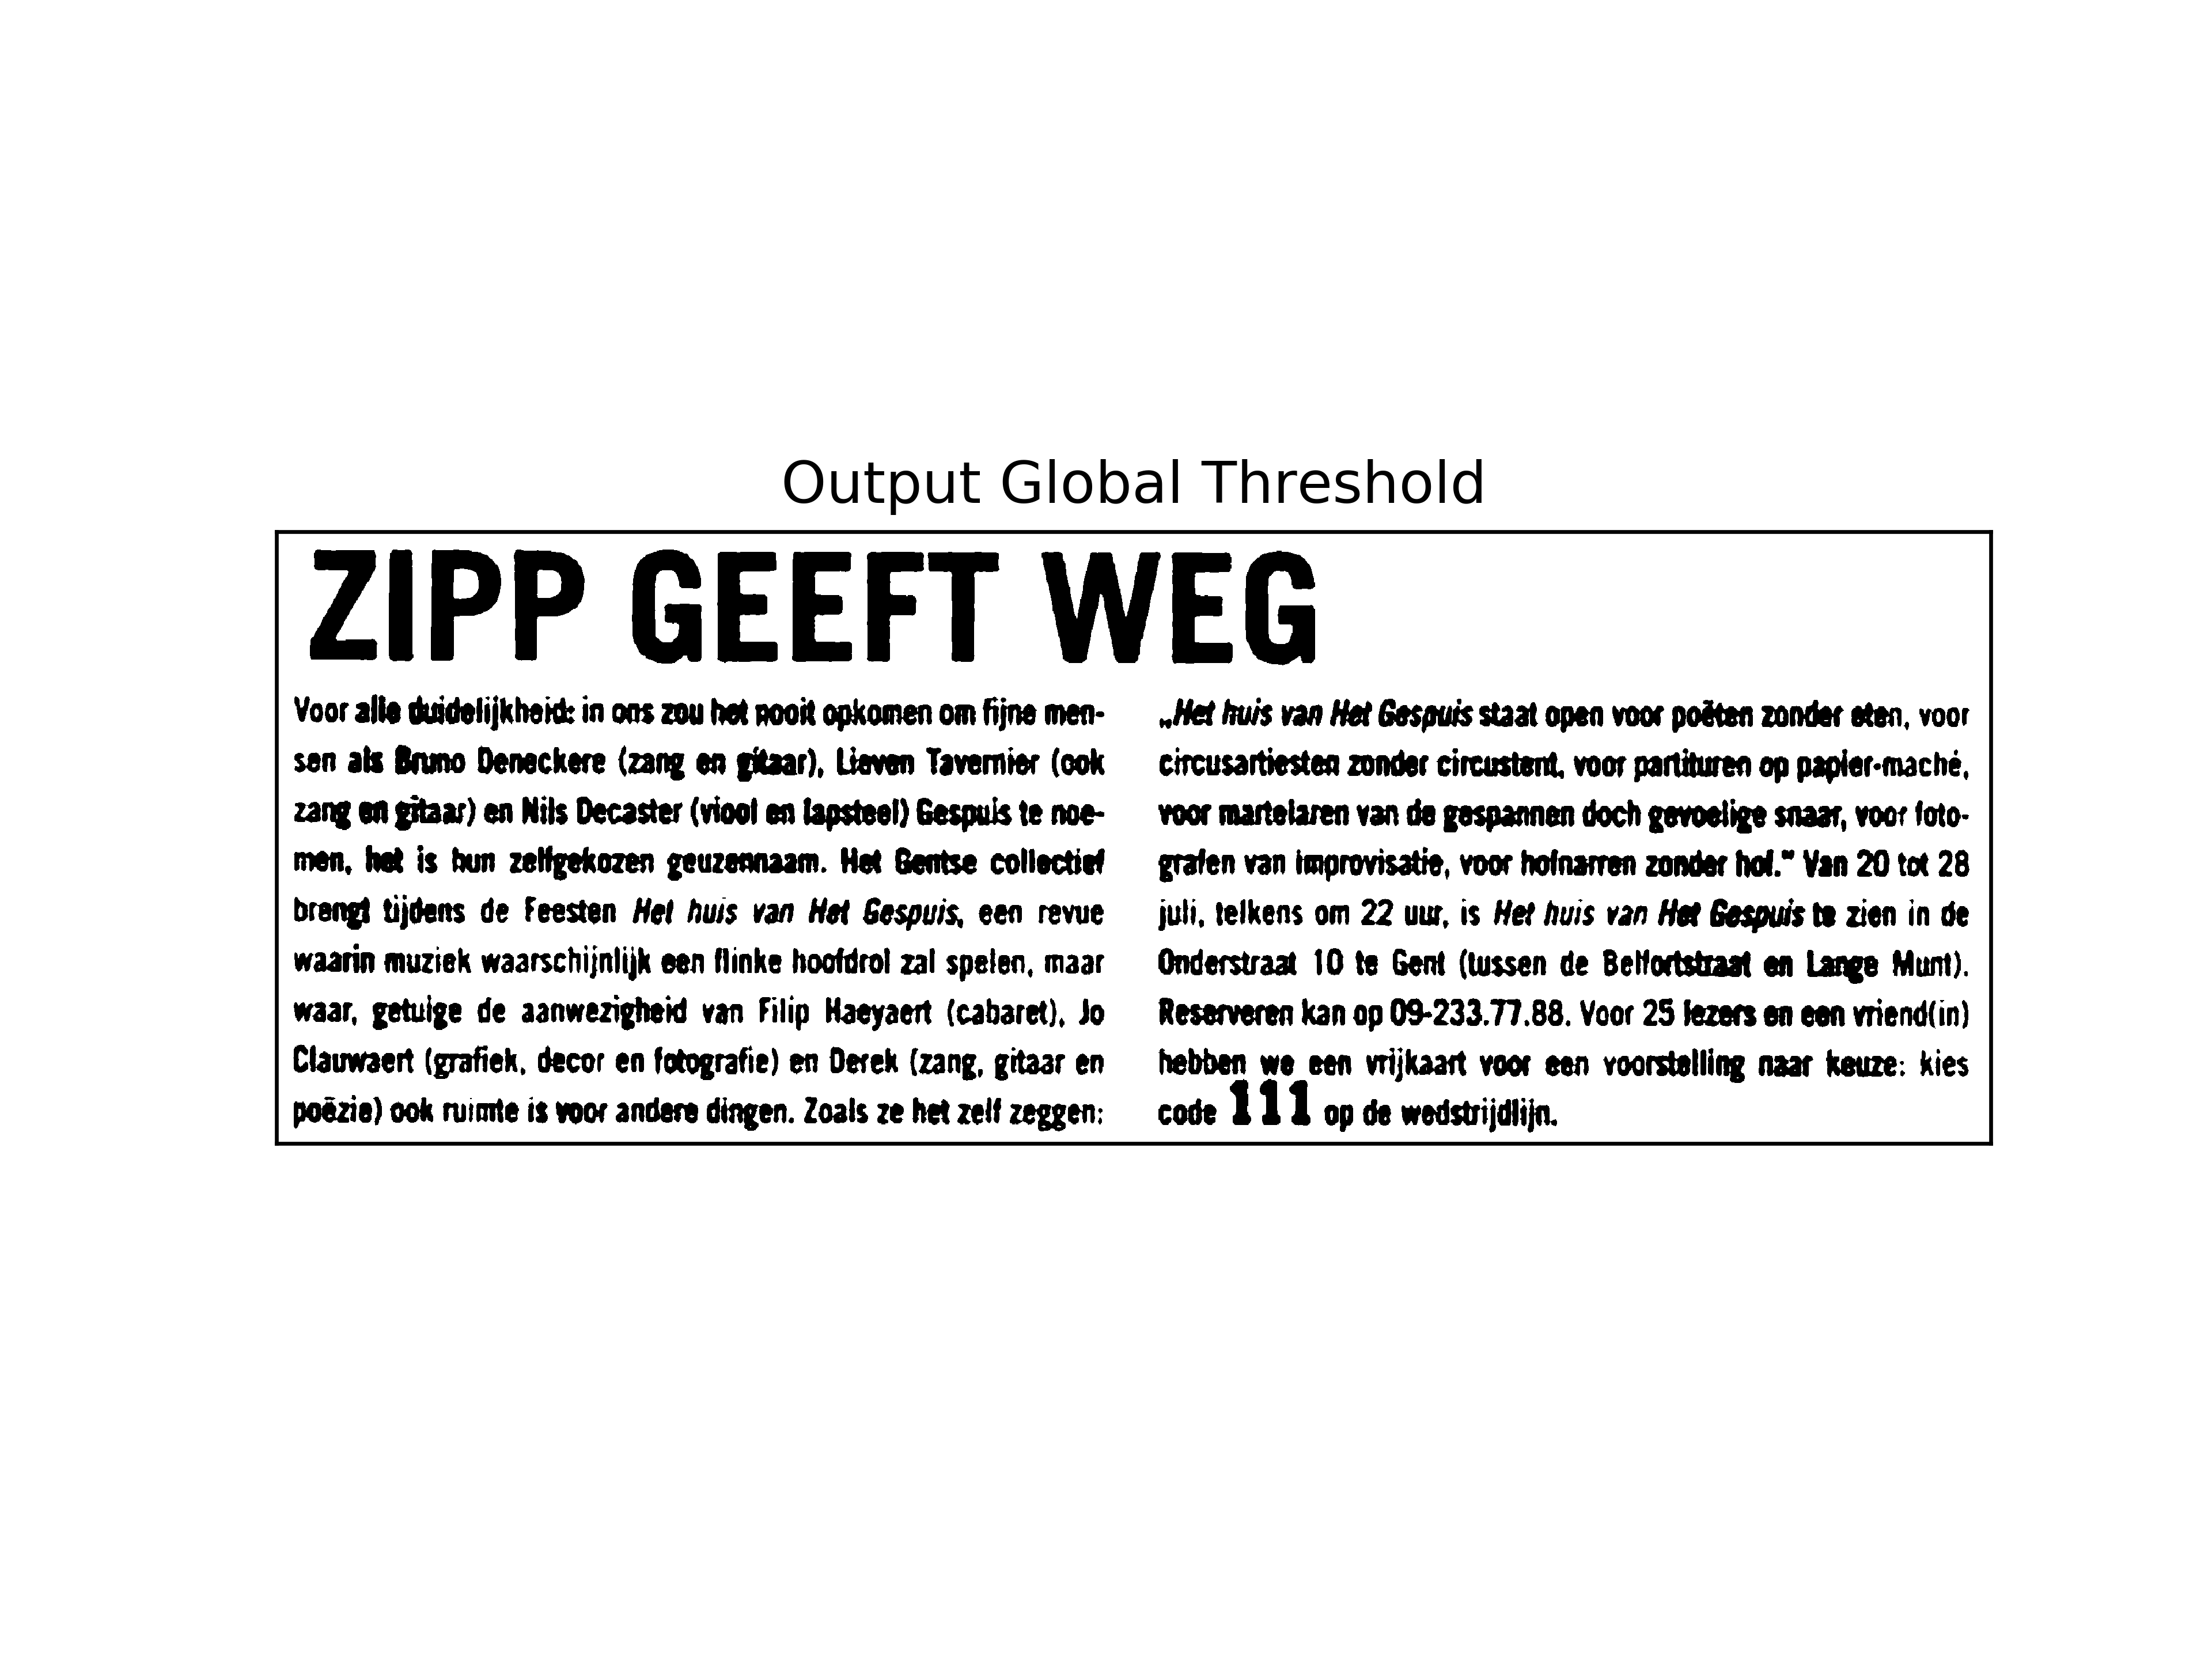
\includegraphics[width=0.32\textwidth]{img_8_output_thresh.png}
\end{center}

Image 9 uses the procedures which are similar to that of image 4 and 5 except
the contrast stretching being applied first. Matlab function 'stretchlim' and
'imadjust' is used for contrast stretching through Matlab Python API. The
'rad' value of the Otsu's threshold function has to be set to 30 for better
text resolution. However, as what I mentioned before, a smaller window size
can cause much more black spot on the background due to the noise on the
image. One way to eliminate these black spot is applying a mask of the line of
text on the processed image. To generate the line mask, firstly, n-bit slicing
is applied on the original image to extract the background pixels. Next, a
line detection kernel can be applied on the image to get the text line
position.

\begin{listing}
\begin{verbatim}
# Image 9 
mat = matlab_func.MatlabFunction()
im_step_1 = mat.contrast_stretch(im_original_gray)
im_step_2 = mf.otsu_threshold(im_step_1, 30)
im_final = mf.line_mask(im_step_2, im_original_gray)
\end{verbatim}
\centering
\caption{List 10: Setting For Image 9}
\newline
\end{listing}

\begin{listing}
\begin{verbatim}
def contrast_stretch(self, im_np):
    im_mat = matlab.double(im_np.tolist())
    img = self.eng.mat2gray(im_mat)
    low_high = self.eng.stretchlim(img)
    out = self.eng.imadjust(img, low_high, [])
    out_np = self.mat2np(out) * 255.
    return out_np.astype(np.uint8)

def mat2np(self, in_array):
    out_array = []
    for _ in range(in_array.size[0]):
        lst = in_array._data[_::in_array.size[0]].tolist()
        out_array.append(lst)
    out_np = np.array(out_array)
    return out_np
\end{verbatim}
\centering
\caption{List 11: Constrast Stretching}
\newline
\end{listing}

\begin{listing}
\begin{verbatim}
def line_detector(im_np, direction='|'):
    line_h = np.array([[-1,-1,-1],
                      [2,2,2],
                      [-1,-1,-1]])
    line_v = np.transpose(line_h)
    line_45p = np.array([[2,-1,-1],
                        [-1,2,-1],
                        [-1,-1,2]])
    line_45n = np.array([[-1,-1,2],
                        [-1,2,-1],
                        [2,-1,-1]])
    if direction == '-':
        im_out = signal.convolve2d(im_np, line_h)
    elif direction == '|':
        im_out = signal.convolve2d(im_np, line_v)
    elif direction == '+':
        g_h = signal.convolve2d(im_np,line_h)
        g_v = signal.convolve2d(im_np,line_v)
        im_out = np.sqrt(g_h**2 + g_v**2)
    elif direction == '/':
        im_out = signal.convolve2d(im_np, line_45p)
    elif direction == '\\':
        im_out = signal.convolve2d(im_np, line_45n)
    elif direction == 'X' or 'x':
        g_h = signal.convolve2d(im_np,line_45p)
        g_v = signal.convolve2d(im_np,line_45n)
        im_out = np.sqrt(g_h**2 + g_v**2)
    elif direction == '*':
        g_h = signal.convolve2d(im_np,line_h)
        g_v = signal.convolve2d(im_np,line_v)
        s_h = signal.convolve2d(im_np,line_45p)
        s_v = signal.convolve2d(im_np,line_45n)
        im_out = np.sqrt(g_h**2 + g_v**2 + s_h**2 + s_v**2)
    return im_out[1:-1, 1:-1]

def line_mask(im_np, im_np_original, window=4, eta=2):
    def _generate_mask():
        im_np_sliced = pp.n_bit_plane_slice(im_np_original, 1)
        im_mask = np.uint8(line_detector(im_np_sliced, direction='+')) // Use horizontal and vertical line mask 
        im_height, im_width = im_mask.shape
        thresh = eta * 255 / ((window * 2) ** 2)
        for m in range(window, im_height-window, window*2):
            for n in range(window, im_width-window, window*2):
                if np.mean(im_mask[m-window:m+window, n-window:n+window].flatten()) > thresh:
                    im_mask[m-window:m+window, n-window:n+window] = 255
        return im_mask
    mask = _generate_mask()
    new_im_np = np.copy(im_np)
    im_height, im_width = new_im_np.shape
    for m in range(im_height):
        for n in range(im_width):
            if mask[m, n] == 0:
                new_im_np[m, n] = 255
    return new_im_np 
\end{verbatim}
\centering
\caption{List 12: Masked Image}
\newline
\end{listing}

\begin{center}
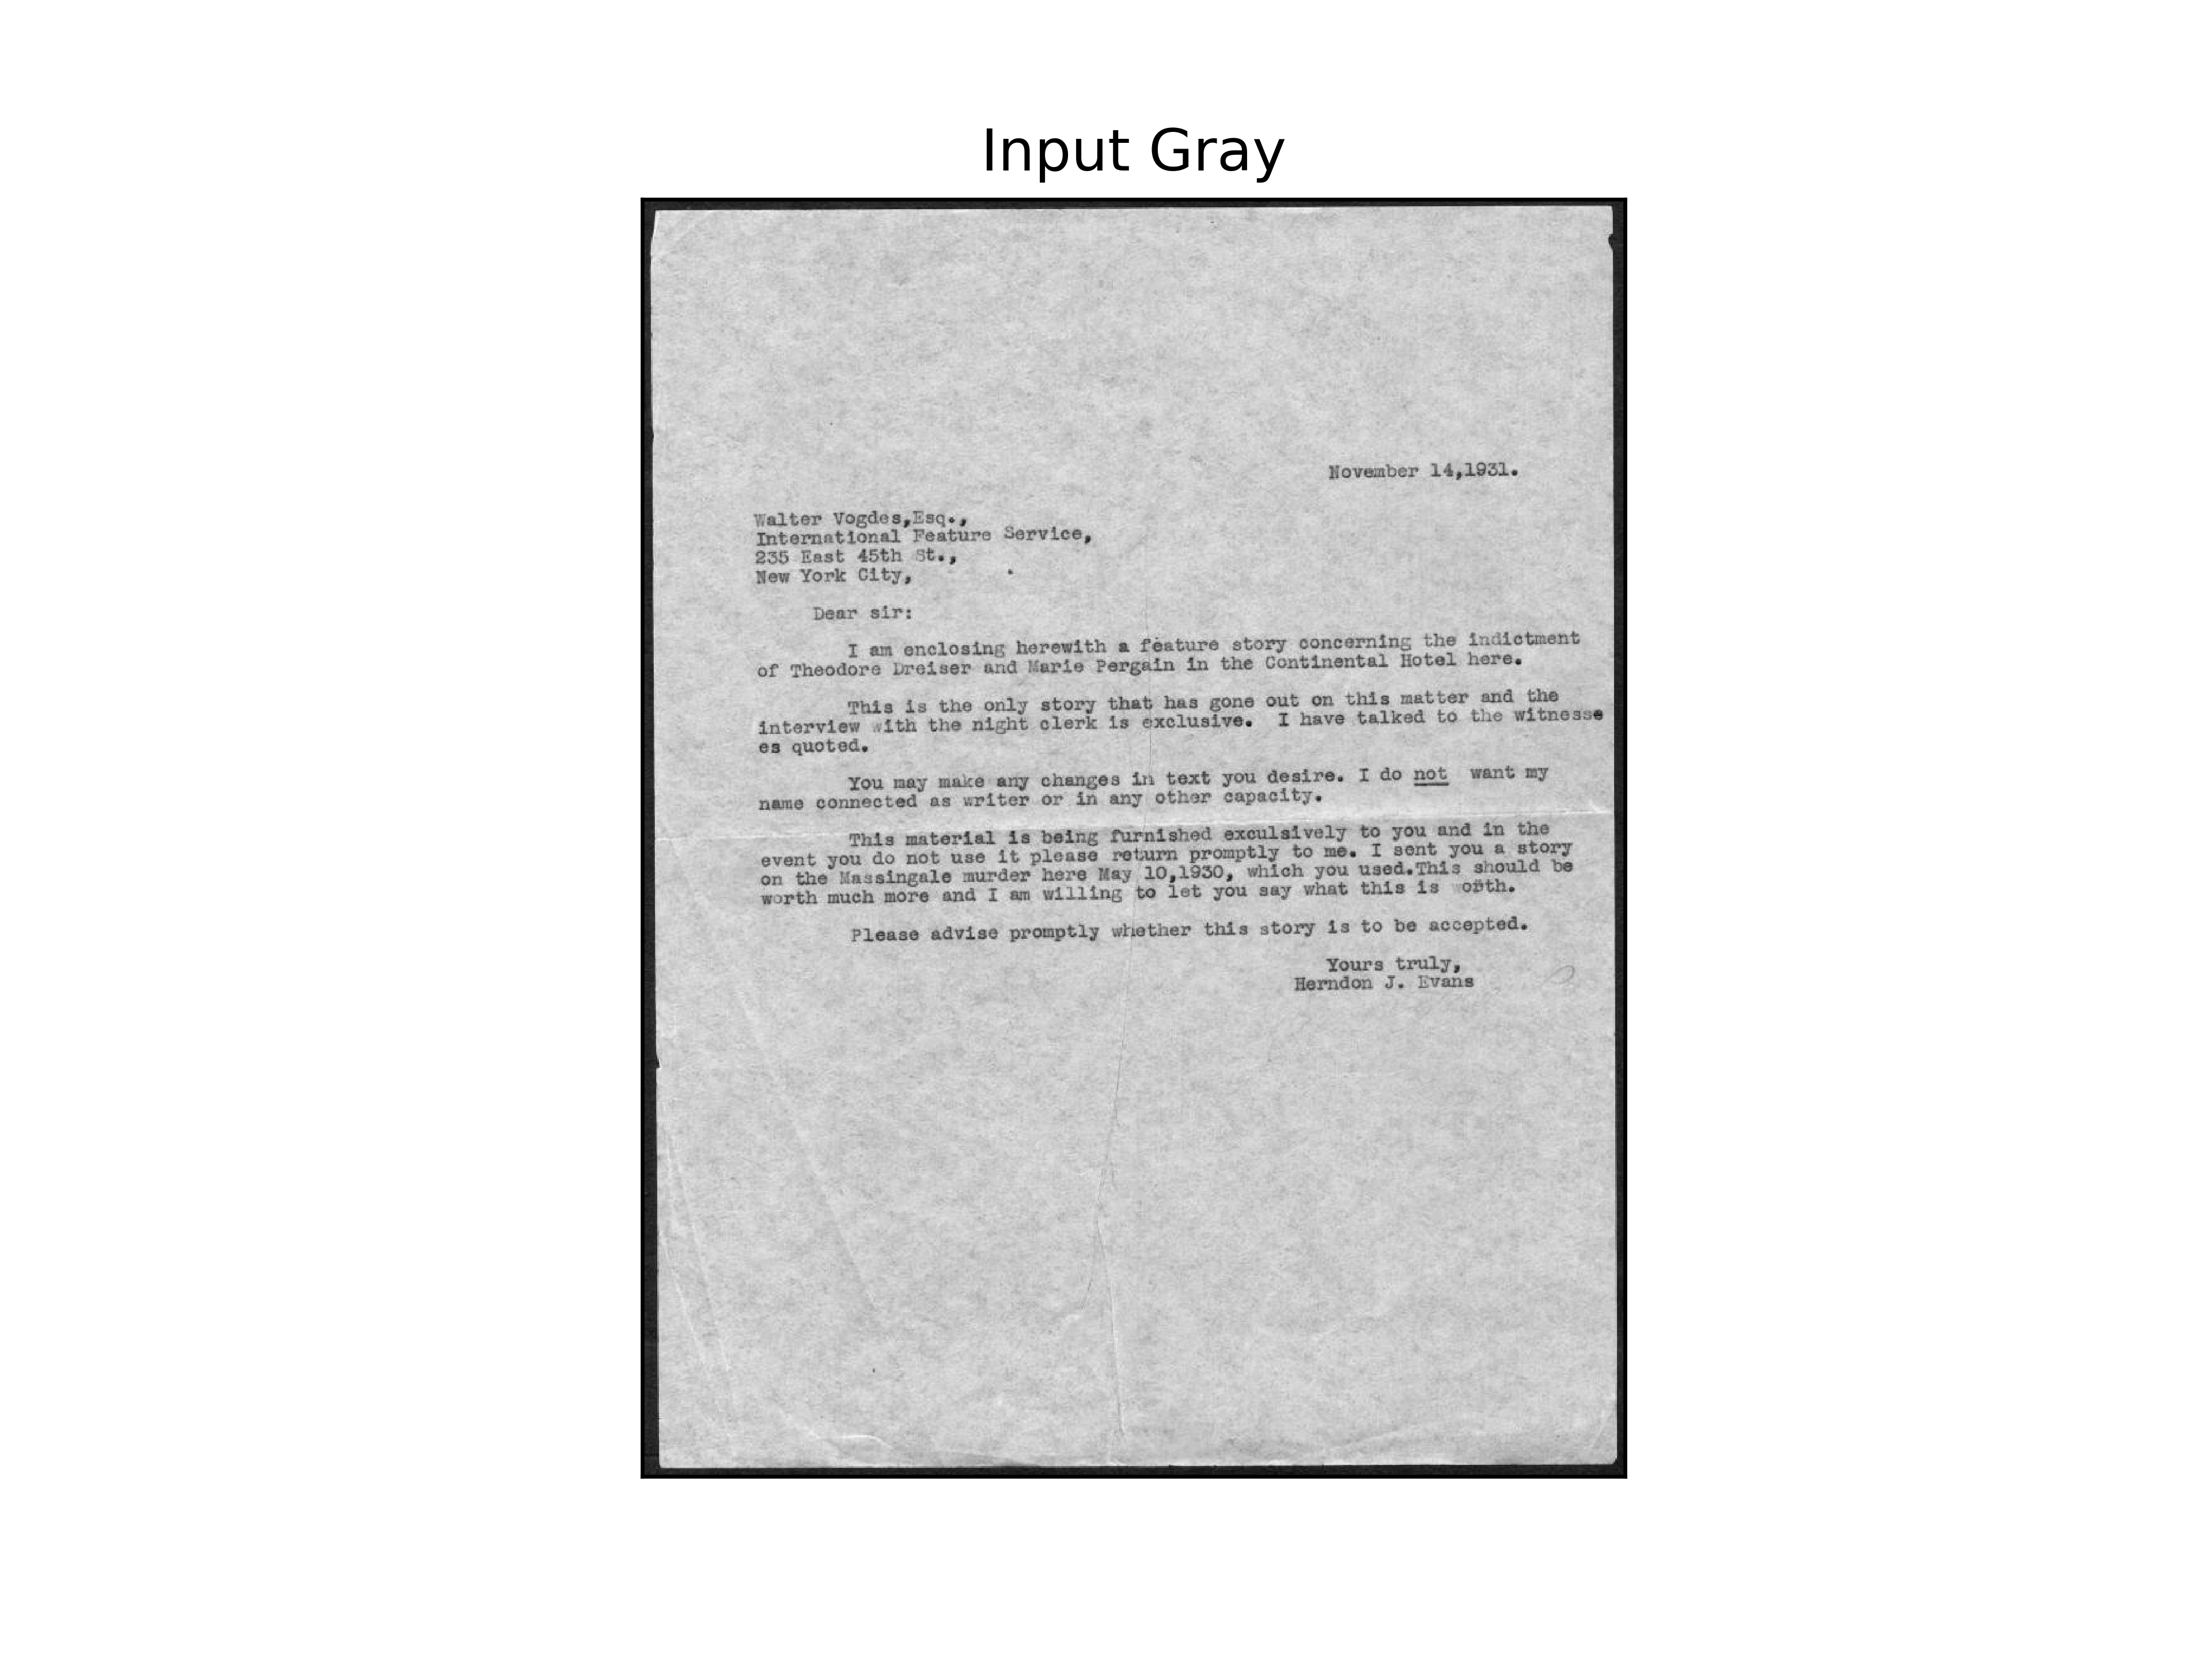
\includegraphics[width=0.49\textwidth]{img_9_gray.png}
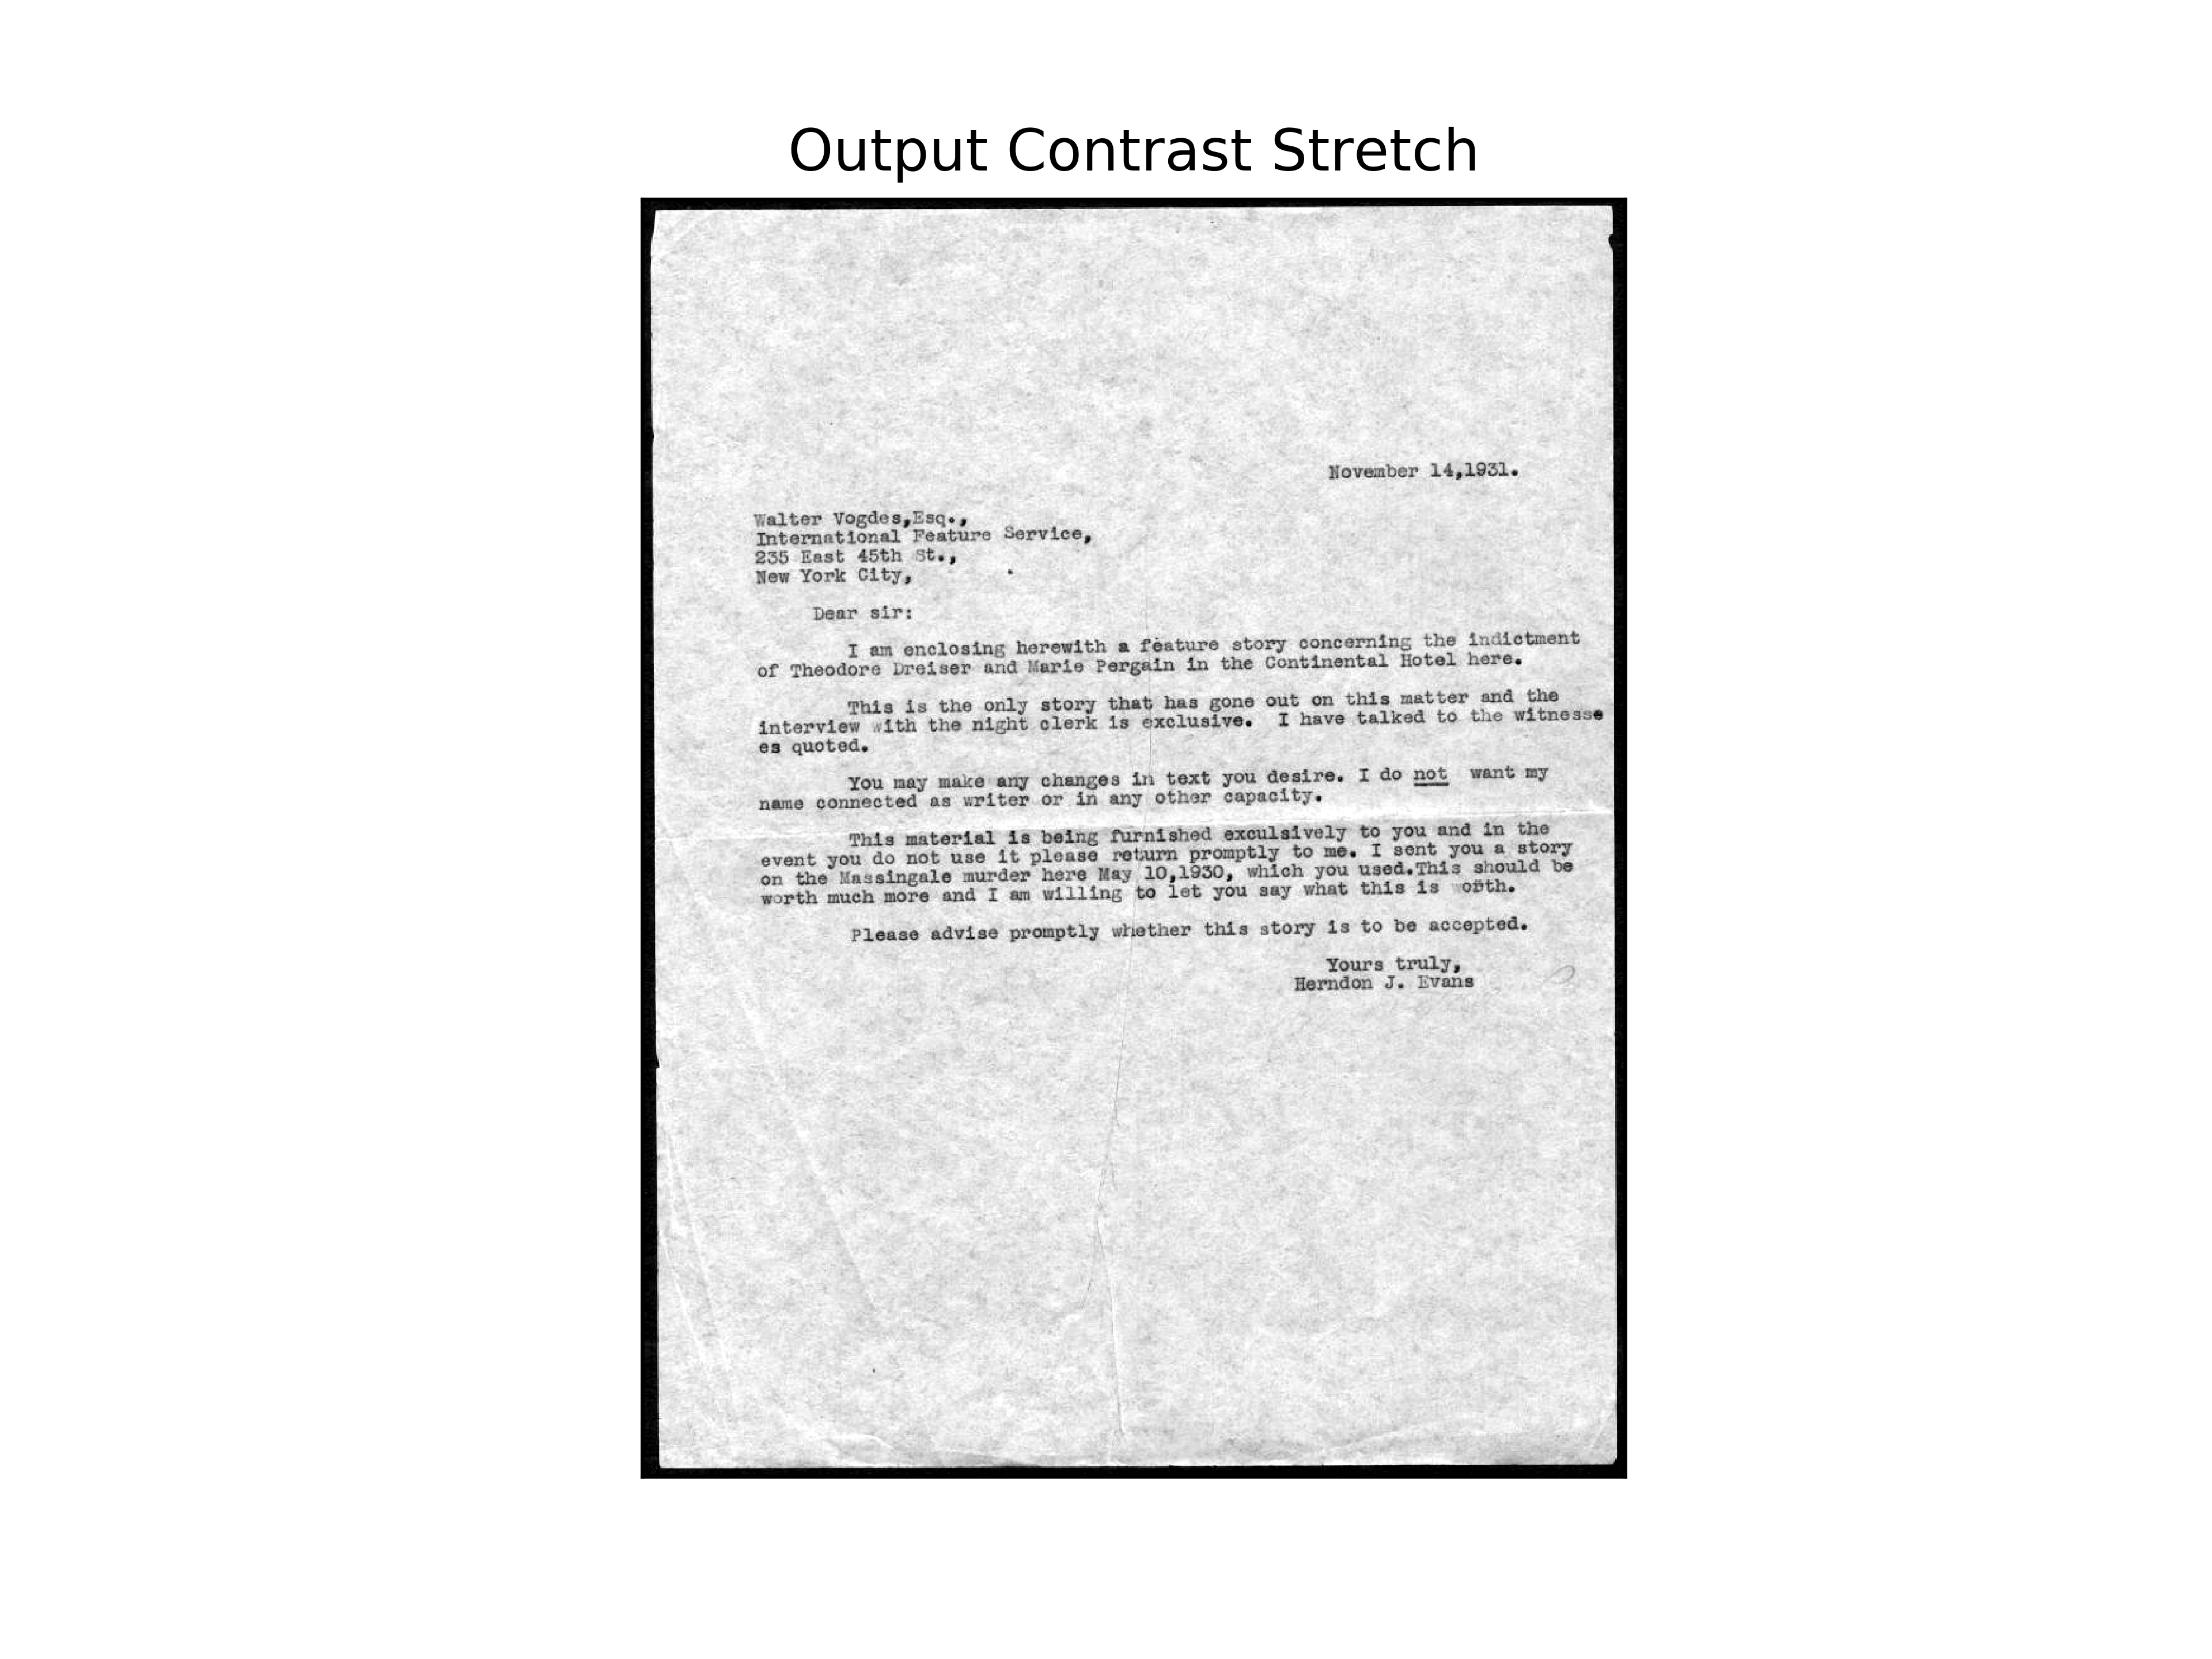
\includegraphics[width=0.49\textwidth]{img_9_output_cont.png}
\end{center}

\begin{center}
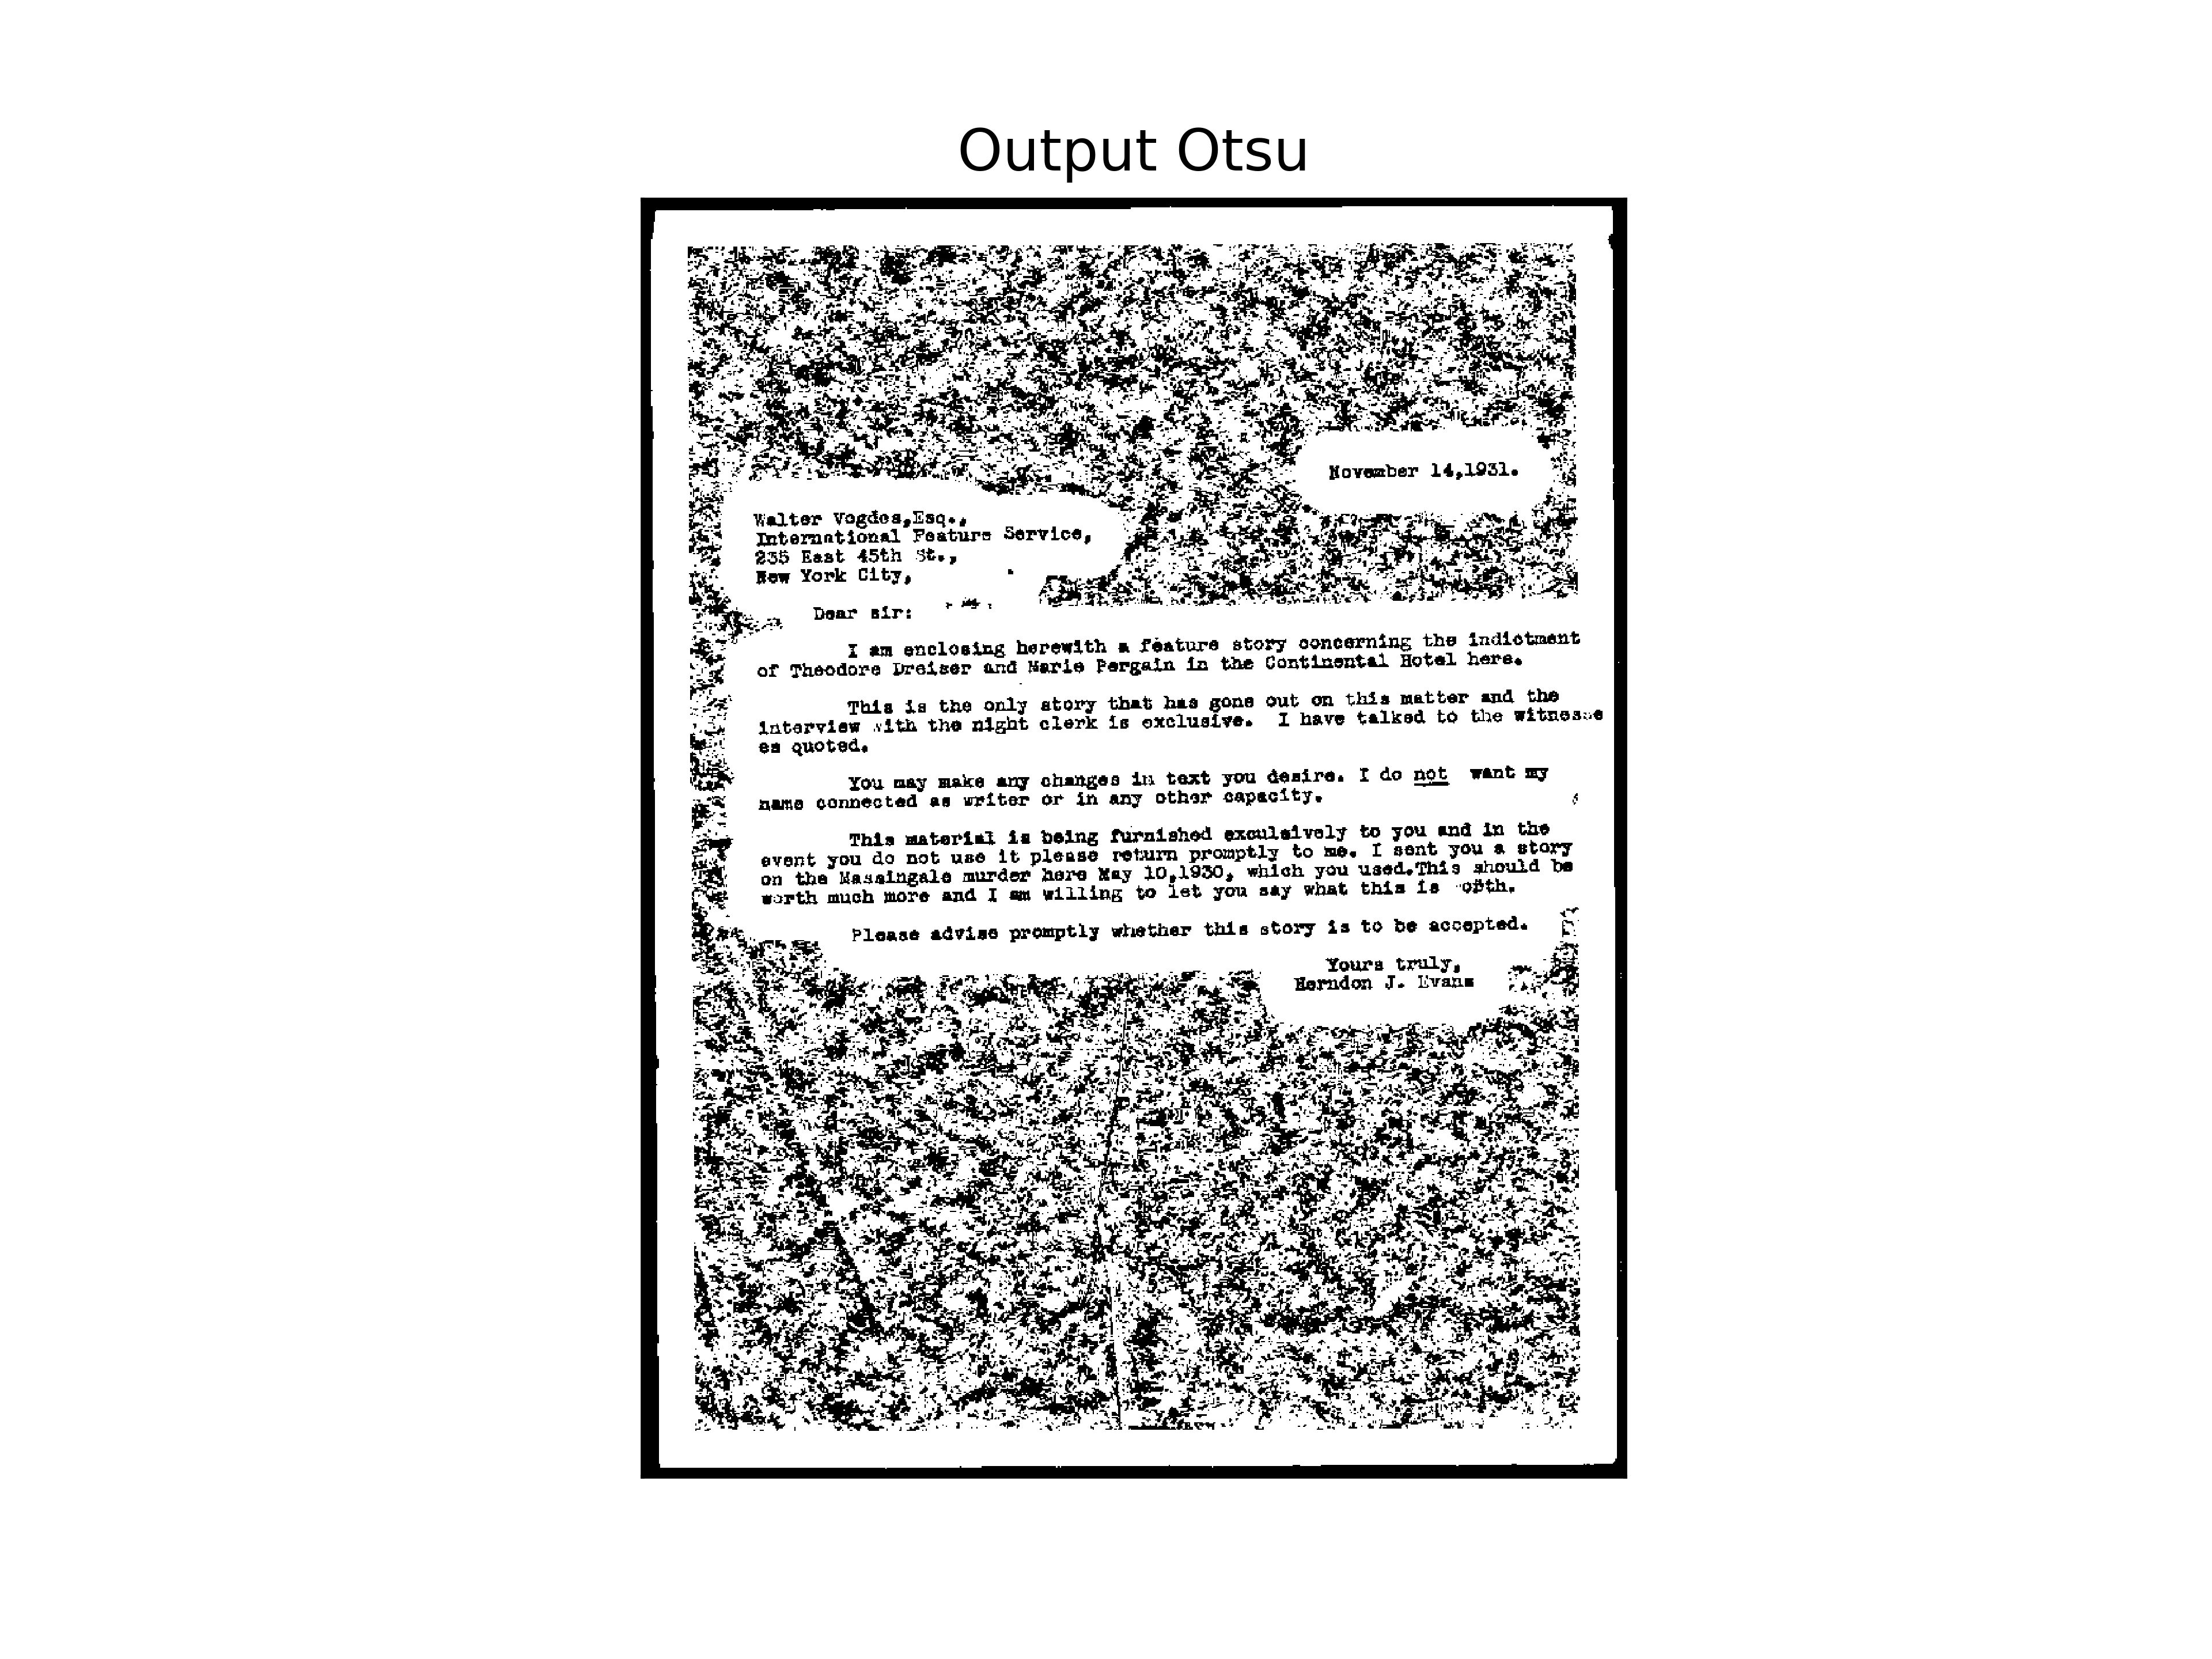
\includegraphics[width=0.32\textwidth]{img_9_output_otsu.png}
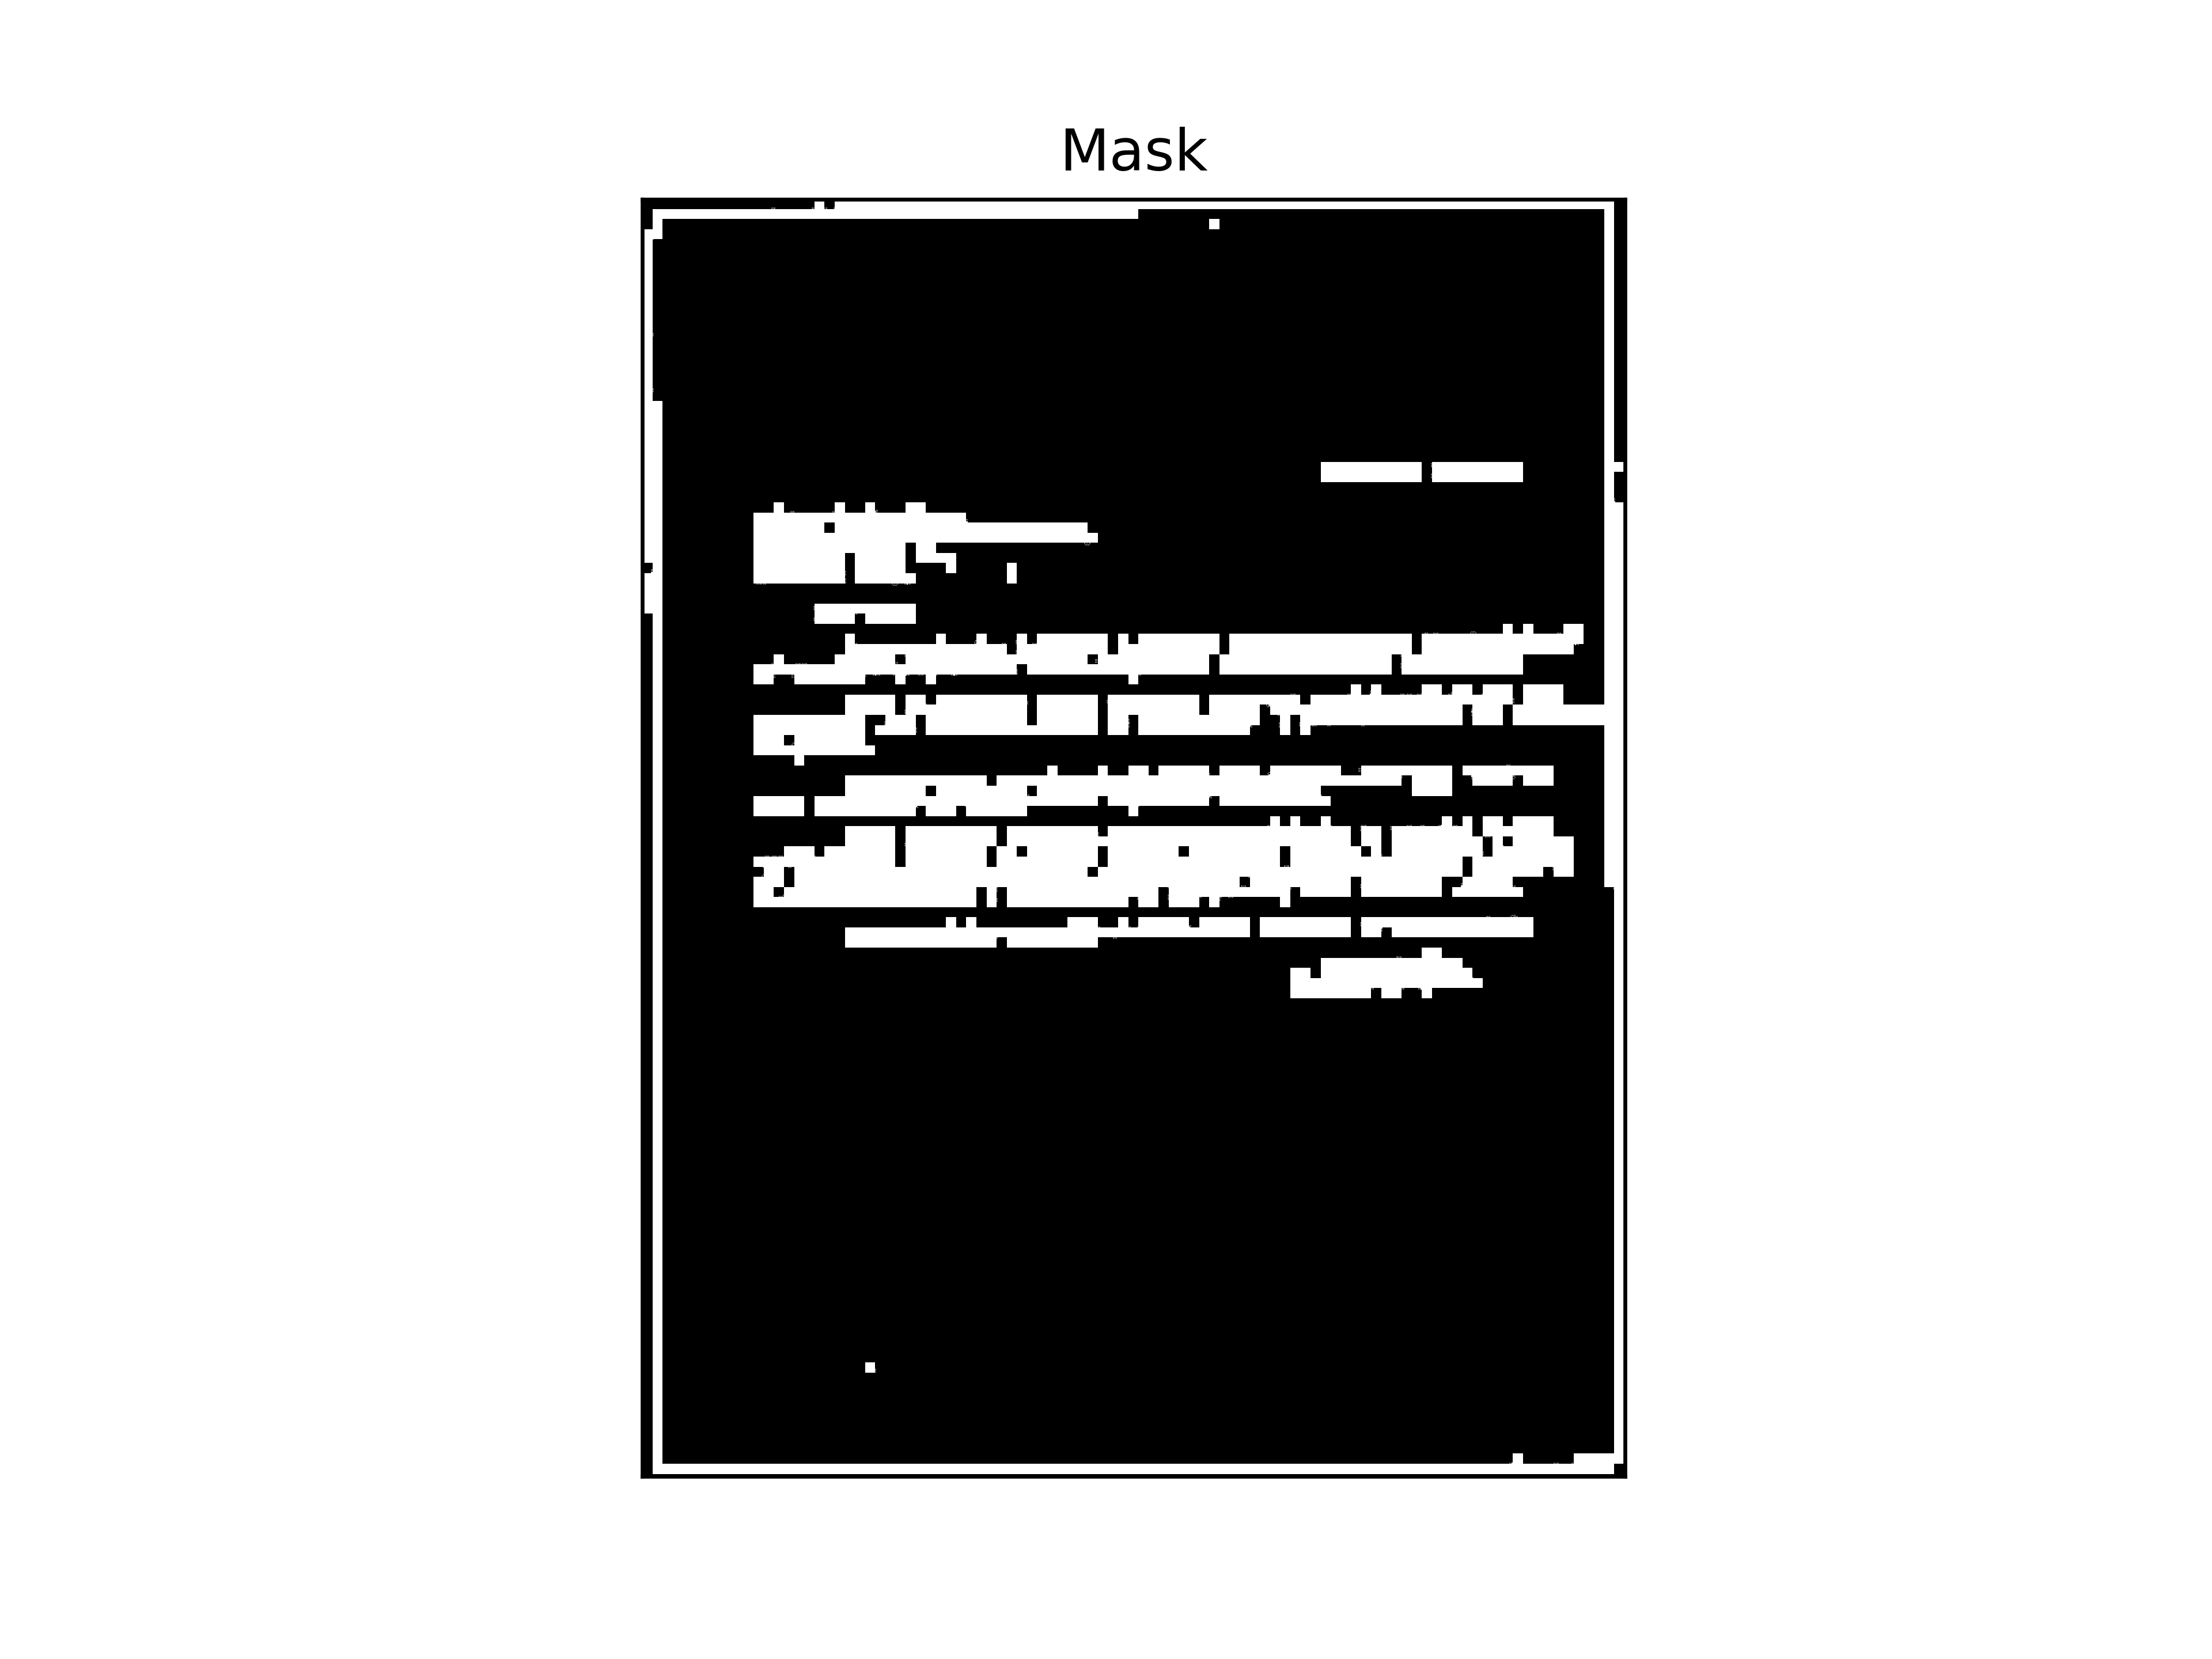
\includegraphics[width=0.32\textwidth]{img_9_mask.png}
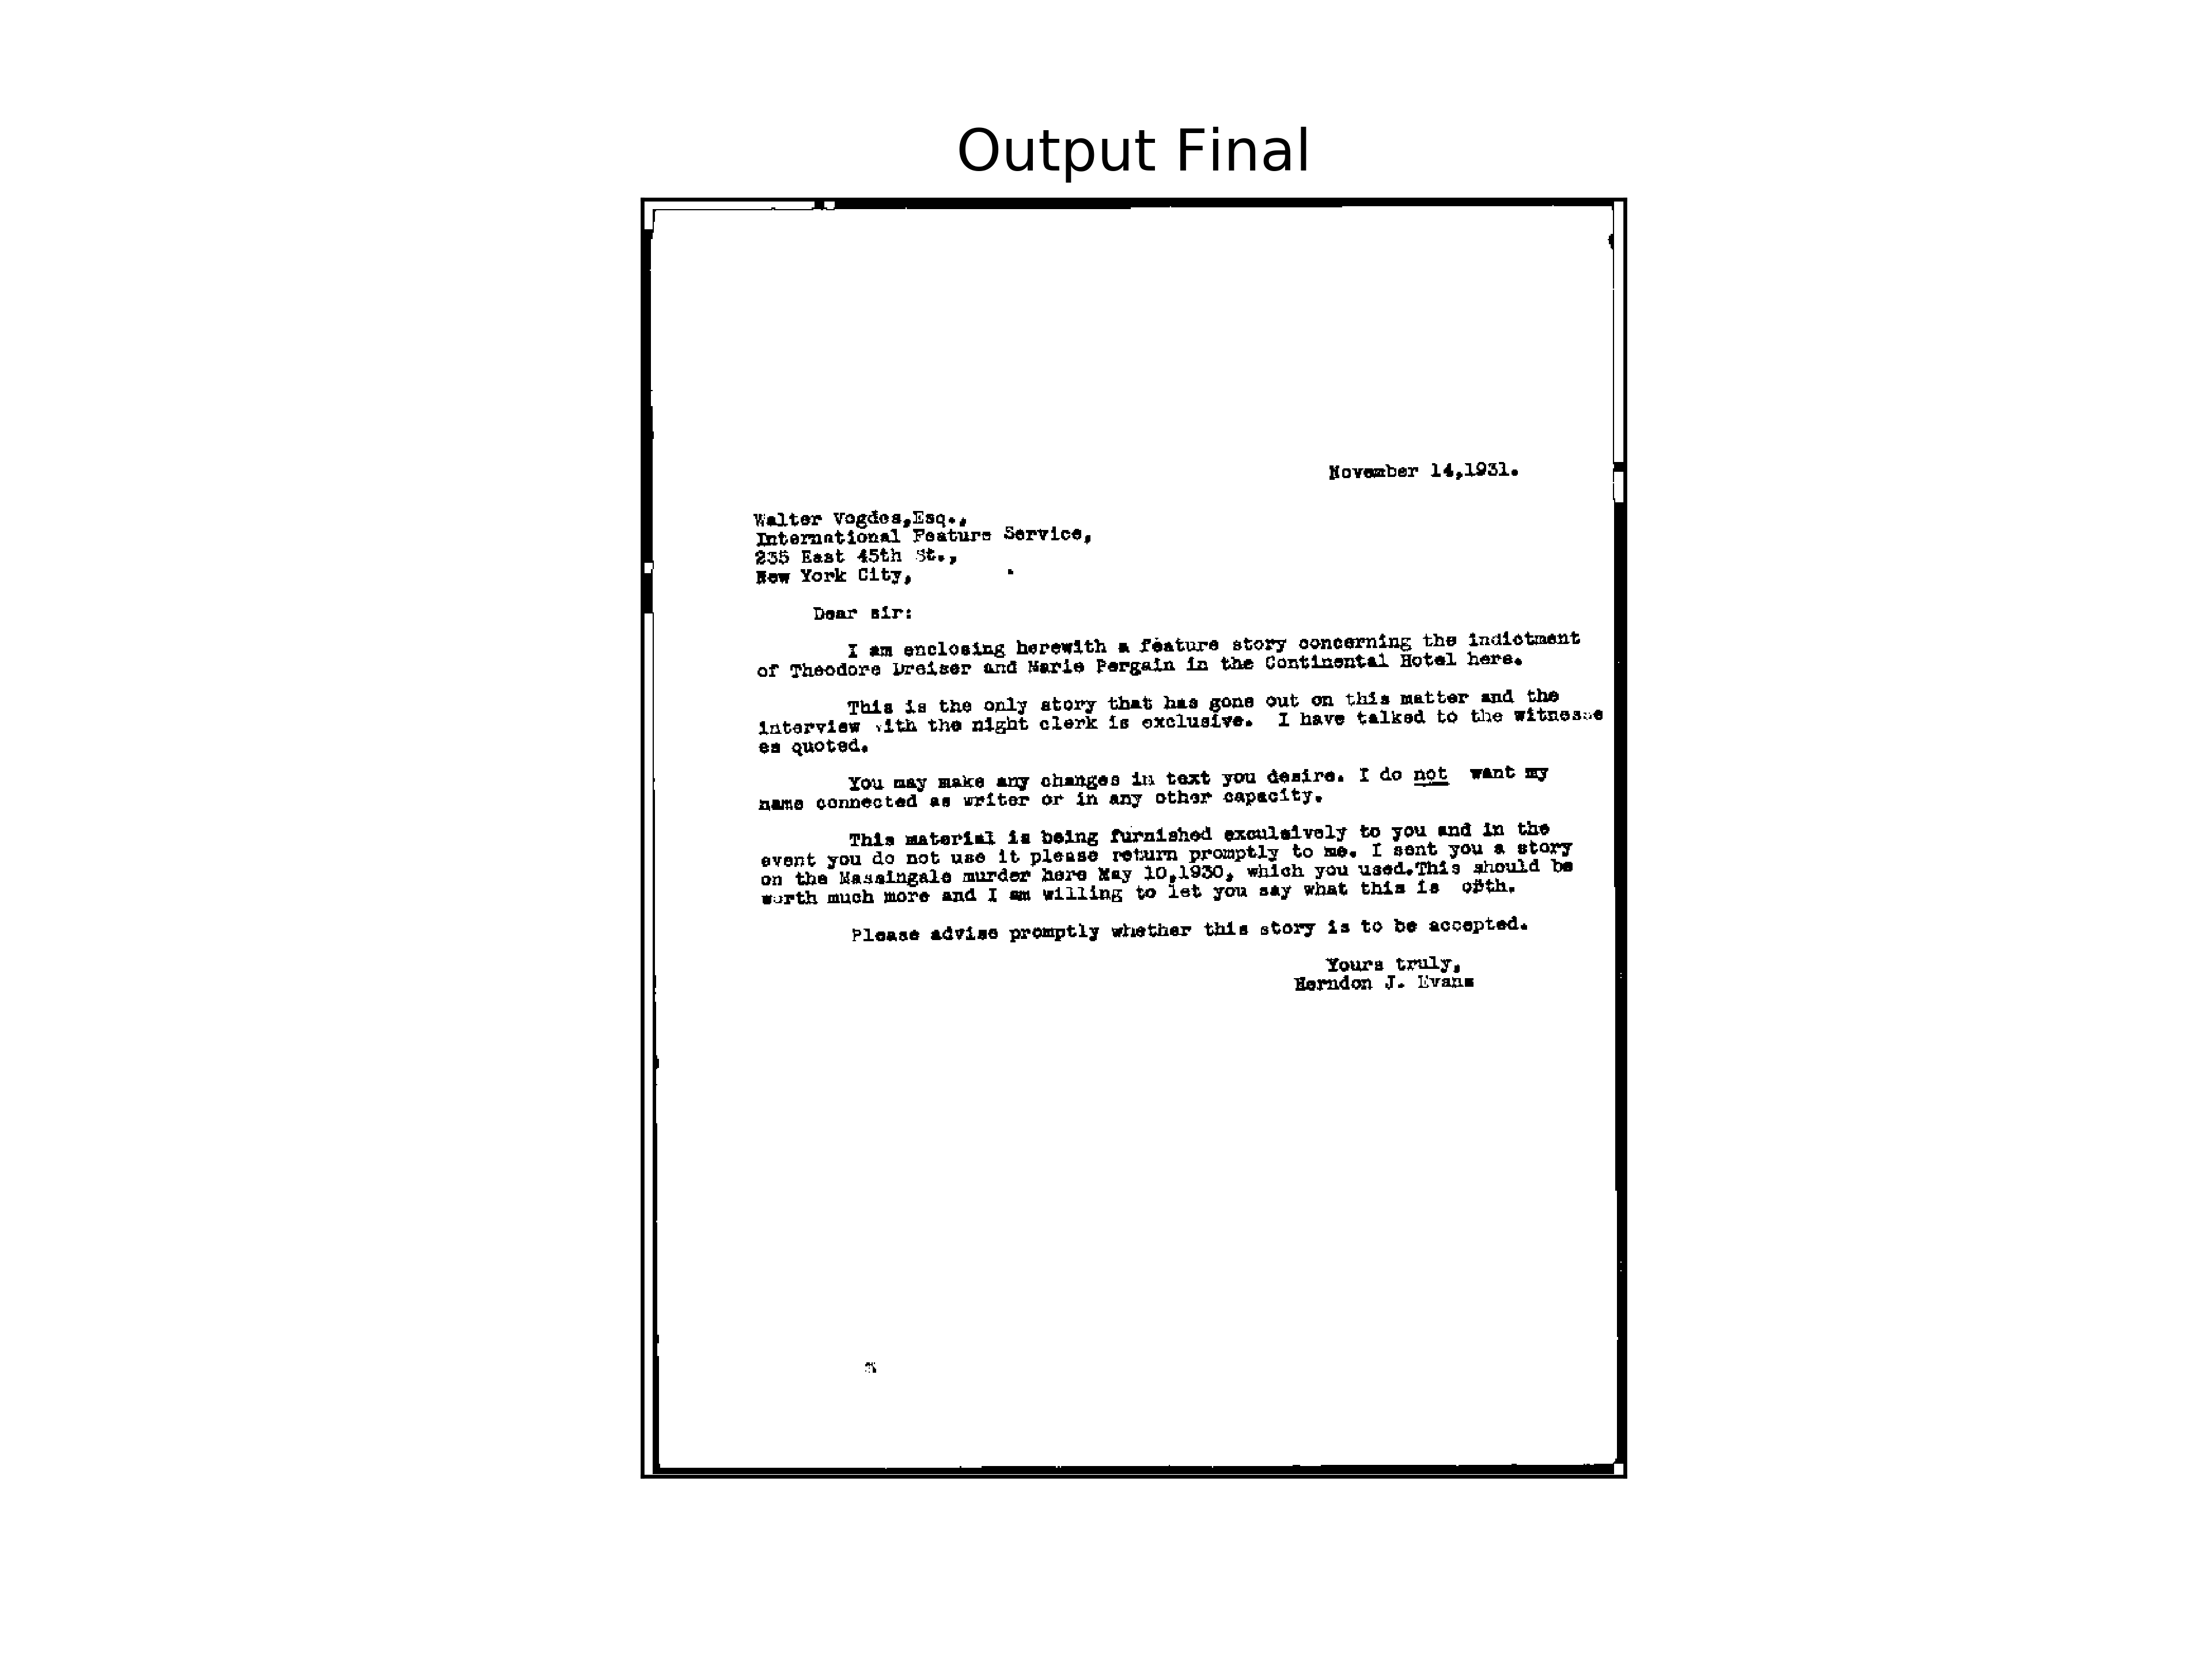
\includegraphics[width=0.32\textwidth]{img_9_output_final.png}
\end{center}

\section{Conclusion}
\label{sec:orgf4833ea}
In summary, the processed images have better resolution for OCR, even though
some small block of text area failed the test. After experimenting different
methods, what I found is that n-bit slicing can handle most of the high
contrast images. Local Otsu's threshold can eliminate shadow on image, however
it also brings some side effect like the black spot. Global threshold has
result similar to that of n-bit slicing.


\addcontentsline{toc}{section}{References}

\begin{thebibliography}{5}

\bibitem{1}\textsc{GitHub} (2017) Pillow [online] Available at: http://pillow.readthedocs.io/en/4.3.x/index.html

\bibitem{2}\textsc{GitHub} (2017) Scikit-Image [online] Available at: http://scikit-image.org/docs/dev/

\bibitem{3}\textsc{MathWorks} (2017) MATLAB API for Python
\newline
[online] Available at: https://www.mathworks.com/help/matlab/matlab-engine-for-python.html 

\end{thebibliography}


\begin{appendices}

\chapter{Souce Code Link}
https://github.com/seanhxx/schoolwork/tree/master/ee4476-imp/assign1

\chapter{Images Link}
https://github.com/seanhxx/schoolwork/tree/master/ee4476-imp/assign1/export

\end{appendices}
\end{document}
